% ================================
% Landon Buell
% Kevin Short
% Physics 799
% 26 September 2020
% ================================


\documentclass[12pt,letterpaper]{article}

\usepackage{amsmath}
\usepackage{amssymb}

\usepackage{algorithm}
\usepackage{algorithmic}

\usepackage{float}
\usepackage{caption}
\usepackage{subcaption}
\usepackage{graphicx}
\usepackage{xcolor}

\usepackage{multicol}

\usepackage[top=2.5cm,left=2.5cm,right=2.5cm]{geometry}

\usepackage{fancyhdr}
\pagestyle{fancy}
\fancyhf{}
\lhead{Landon Buell}
\rhead{B.S. Physics Thesis}
\cfoot{\thepage}

% ================================

\DeclareMathOperator{\sign}{\text{sign}}

\setcounter{tocdepth}{2}

% ================================

\begin{document}

% ================================================================
% ================================================================

\begin{titlepage}
	\begin{center}
   		\vspace*{1cm}
       	\begin{LARGE}
       	\textbf{Audio Classification of Musical Instruments with a Multimodal Neural Network} \\
       	\end{LARGE}
       	\vspace{6cm}

       	\textbf{By: \\ Landon Buell$^1$} \\       
       	\vspace{0.5cm}
       	\textbf{Advised By: \\ Dr. Kevin Short$^2$ , Dr. Maurik Holtrop$^1$} \\
      	\vspace{1cm}
      	A thesis presented for the degree of\\
       	Bachelor of Science in Physics \\
       	\vspace{0.5cm}
       	\textbf{December 2020}
        \vspace{1cm}

       	\vfill
      
       	\vspace{1cm}              
       	$^1$Department of Physics and Astronomy\\           
       	$^2$Department of Mathematics and Statistics\\
       	\vspace{0.5cm}  
       	University of New Hampshire\\
       	Durham New Hampshire, USA\\            
   \end{center}
\end{titlepage}

% ================================================================
% ================================================================

\newpage 
 
\begin{abstract}

The task of recognizing the source of a sound wave in a digital audio file is trivial and almost effortless to a human being in many cases, but is far more difficult for a computer to do. In order to automate source source identification, we have designed and constructed a multimodal neural network that can classify audio files by what musical instrument the sound most resembles. The network uses two different input branches, one being a convolutional neural network (CNN), and the other, a multilayer perceptron (MLP). The CNN branch accepts input in the form of a two-dimensional spectrogram matrix, which encodes the energy distribution of an audio signal over frequency and time, and the MLP branch accepts input as a one-dimensional array of features derived from the physical nature of the sound wave. The spectrogram is produced by using a concatenation of multiple short-time Fourier transformations (STFT) of overlapping windowed time-space analysis frames. The feature vector implements techniques from digital signal processing to combine more explicit properties of the time-space and frequency-space information. To classify the audio files based on predicted sources, we aggregate and transform the activations from the final layers of each branch, and produce a single prediction label. We find that this architecture allows for reasonable classification performance, and demonstrates superior classification performance on average, when compared to either of it's constituent unimodal architectures. Training data for this experiment is from studio recordings of the Philharmonia Symphony Orchestra and the University of Iowa's Electronic Music Studios.

\end{abstract}

\vspace{8cm}

\begin{center}
All source code and documentation for this project can be found at  \\
\textit{https://github.com/landonbuell/Buell-Senior-Thesis}
\end{center}


% ================================================================
% ================================================================

\newpage 

\tableofcontents

% ================================================================
% ================================================================
\newpage
\section{Introduction}
\label{sec-Introduction}

% ================================================================

\subsection{Introduction}

\paragraph*{}The ability to classify time-series data into unique categories has become topic of much attention in the last few decades \cite{Khan,Mierswa}. From climate measurements, to financial reports, to audio-visual media, or to medicine, time-domain signals surround the modern world at every corner \cite{Virtanen}. In each context, the general idea is to place information into distinct categories called \textit{classes} based on inherent properties of the data. For example, doctors may wish to classify a patient as having a heart condition based on properties of their heartbeat or banks may wish to classify a purchase as fraudulent based on a history of spending habits. Often, the volume  of information or complexity of the task makes it unreasonable for a human to do without the aide of some form of automation.

\paragraph*{}It has long been a goal of computer scientists and engineers alike to develop a program, algorithm, or machine that could perform a certain task to the level of human-being \cite{Bishop,Geron,Loy}. While humans are intricate organisms capable of recognition or classification in many contexts, we do not have the ability to process millions of raw numerical values in the course of a few seconds. Similarly, modern computers are also complex systems that can filter through exabytes of information on a daily basis, but are not generally known for being able to distinguish cats from dogs \cite{Geron}. The compromise between humans and machines an algorithm called a \textit{neural network} that combines the computation speed of a computer with the decision-making power modeled from human brain \cite{Goodfellow,Levine,Loy}.

\paragraph*{}In this work, we have developed an automated neural network program that can classify digital sound waves as one of $37$ musical instruments that it most closely resembles. The general use of machine learning algorithms for audio information classification or identification is well explored, and a topic of much modern research \cite{Khan,Liu,Mierswa,Serizel,Zhang}. From previous work, it has been found that various types of audio classification are possible, and are still being expanded upon. Many papers detail possible sets of inputs for classifying speech against music or inputs for organizing audio-visual media based on content. In each case these inputs, called features, must often be tailored to meet the specific task at hand \cite{Virtanen,Liu}.

\paragraph*{}It has been experimentally determined that the choice of features is critically important to classification success \cite{Khan,Mierswa,Serizel}. In our case, the nature of these features is motivated by the physics and mechanical properties of each musical instrument class. By exploring the physics of the vibrating parts of each instrument according to the Hornbostel-Sachs classification system, we gain a more thorough understanding of each instrument group. This allows us to develop properties within each class that are consistent and have low variability, and what properties differ between classes and show a higher variability. These differences are key to providing a set of features which allow a neural network to differentiate between classes of musical instruments \cite{Liu,Zhang}. For our classifier model, we have developed $24$ features from the time-series and frequency-series representation of the audio file data. These quantities are assembled into a single axis array for processing. Additionally, we construct an image-like representation of the waveform and the 2D array is also used for proceessing. Both of these input modes represent a set of features that convey the nature of the waveform in two different modalities.

\paragraph*{}As the name implies, a neural network is a computation a model or graph that is loosely structured off of the biological brain \cite{Geron,Loy}. Where a biological brain uses physical connects through axons to exchanges chemicals to communicate information, a neural network uses a chain of mathematical operations to communicate information \cite{Goodfellow}. The earliest work on attempting to model cognitive processes goes back to 1943, where Warren McCulloch and Walter Pitts began to develop a model of the human brain using principles of mathematics \cite{McCulloch,Loy}. Nearly ten years later, a simple neural networks called the \textit{perceptron} was developed by Frank Rosenblatt, which modeled connections of neurons through principles of linear algebra \cite{Geron,Petrik}. Another decade after that, inspiration from the visual cortex gave rise to the convolution operation to be applied to digital image processing. 

\paragraph*{}The design of our neural network function combines two distinct architecture types by using two distinct entry arrays which are processed, and a single output is formed. This type of neural network is referred to as a \textit{multimodal} neural network \cite{Li,Ngiam}. Our model contains a convolutional neural network (CNN) that processes an image-like representation of an audio waveform, and a multilayer perceptron (MLP) that processes a list-like representation of an audio wave form. Each arm of the network is it's own computational graph that is designed to process it's respective inputs types. The activations at the end of each layer are concatenated into a new layer, which is further processed and then used to generate a single prediction. This output that is aggregated from two inputs shows on average, superior classification performance when compared to either of it's constituent unimodal architectures alone.

% ================================================================
% ================================================================

\newpage
\subsection{Methodology}
\label{sec-Methodology}

\paragraph*{}This project includes a number of steps from taking raw input data to the final classification program. In this section, we provide a very high level outline of the parts of this projects and show how each one influence the final product. Additionally, we indicate the sections in this thesis where the particular material is introduced and developed much more thoroughly.

% ================================================================

\subsubsection{Designing the Function}

\paragraph*{}To automate the process of classifying audio files, we require a program or algorithm that can make practical decisions based on a prescribed set of information. This is to say that we need a \textit{function} to process an input or set of inputs, and return a predicted label that corresponds to a musical instrument. Consider the biological process of hearing a sound wave and matching it to a source. We can model this behavior by some unknown function $F$ and approximate it with the function $F^*$. This approximate function is composed of smaller functions that collectively work together to direct the flow of information and allow for the mapping of the contents of a sound file to a potential source as to mimic the behavior of $F$. For a set of inputs $\vec{x} = \big\{ x_0 , x_1 , x_2 , ... , x_{p-1} \big\}$ and a set of classes $0$ through $k-1$, we denote this function as:
\begin{equation}
\label{eqn-MappingFunction}
F^*: \vec{x} \rightarrow \big\{ 0, 1, 2, ... ,k-2, k-1 \big\}
\end{equation}

\paragraph*{}The smaller functions that comprise $F^*$ are called \textit{layers} \cite{Loy,Goodfellow}. Each type of layer performs a different operation and processes different types of input. In secs. (\ref{subsec-NerualNetworkIntro}) and (\ref{subsec-NetworkStructure}), we introduce the nature and structure of a neural network and how it can use used in part to solve this problem. We discuss it is inspired from a biological brain and show how different layer types are influenced from the brain's functions as well as how they are used in this problem. Using information about the problem, we carefully design the inputs, outputs and structure of the neural network function to be able to complete this task in a practical manner. 

% ================================================================

\subsubsection{Collecting and Pre-processing Raw Data}

\paragraph*{}In order to train the neural network to be able to identify musical instrument sources, we need a suitable data set to present to the model as training and validation data. The models uses this data and corresponding labels in the training process to modify it's function to allow for it to complete the task. University of Iowa Electronic Music Studio, and the London-Based Philharmonia Orchestra each have a large collection of publicly available audio files \cite{Philharmonia,UnivIowa}. These files contain short segments of musical instruments performing a single note, and are labeled according to the instrument that produced the sound. The files and labels make up the core of the data set that we use to train the model.

\paragraph*{}To ensure that these data sets are formatted consistently, we have designed a MATLAB program to read each audio file from it's original format, \textit{.AIF}, \textit{.MP3}, or similar, and rewrite the data as a new \textit{.WAV} files, sampled at 44.1 kHz with a 24-bit depth. This ensures that all data will have a consistent format when features are extracted. This stage is detailed in section (\ref{subsubsec-Preprocessing}). After the samples are formatted, we have produced a Python script with iterates through each new file and assigns a class label based on the title of the instrument. This has been design to account for the specific naming cases that arise. We assemble a dictionary-like structure of all training file with organizes the local file location of each sample and provides an integer and string label for all samples. 

% ================================================================

\subsubsection{Designing Classification Features}

\paragraph*{}The performance of a neural network is largely dependent of designing an appropriate set of predictors or features which represent the raw input given to the model. These inputs are designed to represent prolific properties of wave forms that can be expressed by a single or multiple numerical values. We detail these features in section (\ref{sec-Features}). We use tools from physics, mathematics, and signal processing to define and explore a comprehensive set of features that enables a high performance of the classifier. 

% ================================================================

\subsubsection{Designing A Complementary Network Architecture}

\paragraph*{}With the appropriate set of features designed, and the number of output categories determined, we can organize the structure of the neural network function. The shape of the network defines the flow of information and the hypothesis space. The nature of all possible solutions that the trained model could arrive at is subject to the architecture \cite{Goodfellow}. We construct a multimodal neural network, explored in section (\ref{subsec-Architecture}), that processes two distinct entry points derived from the same audio sample. This network is designed to evaluate each input independently, and concatenate the results to produce a single outputted prediction. This hybrid architecture combines the predictive power of the both a multilayer perceptron and a convolutional neural network. Our neural network was implemented using the tools available with the \textit{Tensorflow} module \cite{Tensorflow}.

% ================================================================

\subsubsection{Testing and Evaluating Network Performance}

\paragraph*{}We execute a K-Folds cross validation algorithm to evaluate the performance of the neural network across overlapping subsets of data. This ensures that the model can perform consistently and reliably given small changes in initial conditions. In this stage, we also examine the value of hyper-parameters, activation functions, and layer widths to best compliment the properties of the data set. This process is repeated and expanded upon until we have produced a model with a sufficient performance. We explore this in section (\ref{sec-PerfEval}). Results of all metrics are computed with the \textit{numpy},\textit{scipy}, and \textit{scikit learn} python modules \cite{numpy,scipy,sklearn}. All performance visualizations are produced with the \textit{matplotlib} python package \cite{matplotlib}.

% ================================================================
% ================================================================

\newpage
\section{The Neural Network}
\label{sec-TheNeuralNetwork}

% ================================================================

\subsection{An Introduction to Neural Networks}
\label{subsec-NerualNetworkIntro}

\paragraph*{} Because of the complexity of sound recognition, the challenge arises as to how to build some sort of program that could function at a level above general procedural or explicit instructional rules. Rather than \textit{hard-coding} a set of conditions or parameters for a classification program, we seek an solution that allows for a computer to \textit{learn} from labeled training examples in order \textit{teach} itself \cite{Bishop,Mitchell}. We choose to employ a neural network, which a computer algorithm that is designed to update itself to perform a task with increasing proficiency as it is presented with new information \cite{Geron2,Goodfellow,Levine,Mitchell}.

\paragraph*{}As the name implies, early neural networks were inspired from from the human brain. Former YouTube video classification team lead, and current machine learning consultant, Aurelien Geron writes about the relationship between biological brains and mathematical neural networks \cite{Geron}: 
\begin{quote}
Birds inspired us to fly, burdock plants inspired velcro, and nature has inspired many other inventions. It seems only logical, then, to look to the brain's architecture for inspiration on how to build an intelligent machine.
\end{quote}
The result is a computer program that is reminiscent of the a brain in that it structured much like the brain, and can\textit{learn} from new data. We model operations with collections are artificial neurons that are capable of connect and interacting with other neurons \cite{Levine}. Where a biological brain uses connections of chemical and electrical exchanges to process input and make decisions, the computational counterpart uses arithmetic and numerical exchanges to similarly process input and make decisions \cite{Levine,Bishop}. Where a brain uses physical connection of neurons through axons, the neural network uses mathematical connections of neurons through mathematical operations \cite{Geron,Levine}. We call the numerical value contained within an artificial neuron the \textit{activation} of that neuron \cite{Goodfellow,Geron}. 

\paragraph*{}When a listener hears a sound, millions of neurons in their brain exchanges those chemical and electrical signals in such a way as to be able to identify the source of that sound \cite{Geron,Virtanen}. More conceptually, we can say that a listener is presented with a set of information $x$, which is air molecules vibrating near their tympanic membrane \cite{White,Olson}. That information is then passed into the brain where some function $F$ is used to model the incredibly complex set of neural connections. The output of that function is some label $y$, which the listener associates with a particular source \cite{Olson}. Similarly, we construct a neural network to accept a set of predictors $x$, which is passed into a function $F^*$ that is use to approximate $F$, and produce an output $y^*$, which predicts the source of the audio sample.

\paragraph*{}The neural network function $F^*$ uses a set of parameters $\Theta$, to map those inputs, $x$ to outputs, $y$ \cite{Goodfellow,James,Virtanen}. It is the process of updating the elements in the object $\Theta$ which allow us to train a neural network to perform the desired task. Similarly, it is the process of organizing and connecting neurons in the brain that allow humans to perform any specific task \cite{Geron,Levine}. Over the course of their lives, humans will be able to learn to match sounds to sources with relative ease, given the appropriate labels. In a similar manner, our neural network is presented a collection of predictors from sound files and a complementary set of labels indicating the source of each sound. This type of task is called \textit{classification}, which involves mapping the input data, $x$ to one of $k$ possible \textit{classes}, each represented by an integer, $0$ through $k-1$. Each of the $k$ classes represents a particular musical instrument or sound source that could have produced the sound-wave in the audio file \cite{Goodfellow,Loy,Virtanen}. In this section, we explore the motivation, structure, and training process of a neural network. We implement our neural network with the \textit{Tensorflow} Python package \cite{Tensorflow}.

% ================================================================

\subsection{The Structure of a Neural Network}
\label{subsec-NetworkStructure}

\paragraph*{}A Neural Network is a model of a mathematical function, composed of several smaller mathematical functions called \textit{layers} \cite{Goodfellow,Loy}. Each layer represents an operation that takes an input, and returns an output . The exact nature of this operation can be very different depending on the layer type or where it sits within the network. Typically, a neural network is characterized by a chain-like structure where the output of one layer is fed directly into the input of the next layer \cite{Geron,Goodfellow}. It is this process of transforming inputs successively in a particular order until an output is attained that makes up the core functionality of a neural network \cite{Geron,Loy}. The output of the final layer encodes the "decision" of the model given a particular input.

\paragraph*{}Other than inspiration from the brain, Neural Networks are named \textit{networks} due to their successive chained or nested composition nature. A standard representation of a neural network is often a linked list or computational graph structure \cite{Goodfellow}. This maps out exactly how the repeated compositions are structured and organizes the flow of information in more complicated networks. Each node in the computational graph represents a \textit{layer}, which executes a particular prescribed mathematical function \cite{Goodfellow}. In the case of a \textit{linear, feed-forward} network, such as the one that we implement, information passes in a single direction to produce an output. We can represent this as a graph:
\begin{equation}
\label{eqn-FunctionGraph}
F^*(x) = x \rightarrow f^{(0)} \rightarrow f^{(1)} \rightarrow ..... \rightarrow
f^{(L-2)} \rightarrow f^{(L-1)} \rightarrow y^*
\end{equation}
or as a nested function:
\begin{equation}
\label{eqn-FunctionChain}
F^*(x) = f^{(L-1)}\big[f^{(L-2)}\big[...f^{(1)}\big[f^{(0)}\big[x\big]\big]\big]...\big]\big] = y^*
\end{equation}
The number of layers in a neural network is referred to as the network \textit{depth}. The dimensionality of each layer is referred to as the network \textit{width} \cite{Geron,Loy}.
A network model that contains $L$ unique layers is said to be an $L$-Layer Neural Network, with each layer indexed by a superscipt, $(0)$ through $(L-1)$. Layer $(0)$ is said to be the \textit{input layer} and layer $(L-1)$ is said to be the \textit{output layer} \cite{Geron,Loy}. 

\paragraph*{}Due to the chained nature of the model, the activations from some layer, $(l-1)$, are used to directly produce the activations for the next successive layer $(l)$. The function that represents a layer $(l)$ is given by:
\begin{equation}
\label{eqn-altLayerFunction}
f^{(l)} : x^{(l-1)} \in \mathbb{R} \rightarrow x^{(l)} \in \mathbb{R}
\end{equation}
The array of activations, $x^{(0)}$, is the raw input given the neural network, called \textit{input} activations. Conversely, $x^{(L-1)}$ is referred to as \textit{output} activations \cite{Geron,James,Loy}.

\paragraph*{}Below we outline a standard "forward pass" algorithm for a general feed-forward deep neural network. We presume each layer to be a node in a computational graph that contains a method "\textit{call}" which executes the layer's main function as in Eq. (\ref{eqn-altLayerFunction}). Additionally, each node contains a pointer "\textit{next}" which gives the next layer in the network chain. Each layer should also store it's linear activations, $z^{(l)}$ and it's output activations $x^{(l)}$ for training purposes. This algorithm is adapted from Goodfellow, \cite{Goodfellow}.

\begin{algorithm}[H]
\caption{Forward propagation system in a standard deep neural network. Each layer is presumed to be a node in a linked computational graph. This example has been setup to assume one input layer, and one output layer. Practical implementations should include mini-batches of data as opposed to a single sample.}
\label{alg-FeedForward}

\begin{algorithmic}
\REQUIRE Set of Layer functions $f^{(i)}$, $i \in [0,1,2,3,...,L-1]$.
\REQUIRE Input sample - $x^{(0)}$

Set the current layer to be the input layer: \\
$f^{(i)} \leftarrow f^{(0)}$
\FOR {Layer $i \in [1,2,3,...,L-1]$}
	\item Run "Call" Method with current activations, transform activations:
	\item $x^{(i)}$ = $f^{(i)}$.call($x^{(i-1)}$)
	\item Move to the next layer in the network:
	\item $f^{(i)} \leftarrow f^{(i)}$.next()
\ENDFOR
\item Return the network's output, which are the output activation of the final layer \\
\RETURN $x^{(L-1)}$
\end{algorithmic}
\end{algorithm}

% ================================================================

\subsection{Layers Used in this Classification Model}
\label{subsec-Layers}

\paragraph*{}As stated previously, a neural network is composed of a series of functions that are called in succession to transform features (an input) into predictions (an output). As shown in Eq. (\ref{eqn-altLayerFunction}), each function feeds directly into the next as to form a chain-like computational graph \cite{Goodfellow}. There are multiple type of layers that we use to construct the network in this project, but the two most important are called a \textit{dense} layer and a \textit{convoltuion} layer. These layers each contain a set of parameters which makeupa  subset of the trainable elements in $\Theta$.
These two layer functions can be divided into two portions: (i.) a Linear transformation, with a bias addition, and (ii.) an element-wise activation transformation. The Linear transformation can be given by Eq.(\ref{eqn-LinearTransform}) in the case of a 1D Dense layer (\ref{subsubsec-DenseLayer}) or Eq. (\ref{eqn-LinearTransform2}) in the case of a 2D Convolution layer.
\begin{equation}
\label{eqn-LinearTransform}
z^{(l)} = W^{(l)} x^{(l-1)} + b^{(l)}
\end{equation}
\begin{equation}
\label{eqn-LinearTransform2}
z^{(l)} = \big(W^{(l)} * x^{(l-1)}\big) + b^{(l)}
\end{equation} 
Where $W^{(l)} x^{(l-1)}$ denotes a matrix-vector product, and $\big(W^{(l)} * x^{(l-1)}\big)$ denotes a convolution product. In both cases, $W^{(l)}$ is a \textit{weighting-matrix} or \textit{weighting-kernel} for layer $(l)$, $b^{(l)}$ is the \textit{bias-vector} for layer $(l)$, $z^{(l)}$ are the \textit{linear-activations} for layer $(l)$ and $x^{(l-1)}$ is the final activations for layer $(l-1)$.

\paragraph*{}Step (ii.) is usually given by some \textit{activation function}:
\begin{equation}
\label{eqn-elementActivation}
x^{(l)} = \sigma^{(l)} \big[ z^{(l)} \big]
\end{equation}
Where $x^{(l)}$ is the final activations for layer $l$ and $z^{(l)}$ is given in equation (\ref{eqn-LinearTransform}). $\sigma^{(l)}$ is some activation function which introduces the ability to account for complicated non-linear decision boundaries which the neural network uses to make predictions. The combination of Eq. (\ref{eqn-LinearTransform}) and Eq. (\ref{eqn-elementActivation}), for a layer $l$ , make up the function represented by that layer, as in Eq. (\ref{eqn-altLayerFunction}). In this section, we detail the types of layer functions that are used to produce the classification model in this project.

% ================================

\subsubsection{Dense Layer}
\label{subsubsec-DenseLayer}

\paragraph*{}The Linear Dense Layer, often just called a \textit{Dense} Layer, or \textit{Fully-Connected} layer, was one of the earliest and most common function types used in artificial neural network models \cite{Geron2,Loy,McCulloch}. A dense layer is composed of a layer of \textit{artificial neurons}, each of which holds a numerical value within it, (usually a double-precision floating point number) called the \textit{activation} of that neuron. The activation of a dense layer are given by a linear combination of the layers inputs. This idea was developed from McCulloch and Pitts' work \cite{McCulloch} in attempting to model cognitive processes as mathematical functions by connecting neurons through a series of weighting values. The idea was expanded upon by Frank Rosenblatt in  1957 by combining many dense layers together to form a multilayer perceptron (MLP), which will make up a portion of the network that we have implemented. \cite{Geron,Loy,Levine}.

\paragraph*{}We model a layer of neurons as an array or vector of floating-point numbers. Suppose a layer $(l)$ contains $n$ artificial neurons- we denote the $n$-dimensional array that holds those activations as $x^{(l)}$ and is given by:
\begin{equation}
\label{layer-DenseNeurons}
\vec{x}^{(l)} = \Big[ x_0, x_1, x_2, \hdots , x_{n-2}, x_{n-1} \Big]^T
\end{equation}
The activation of each entry is given by a linear-combination of activations from the previous layer, Eq.(\ref{eqn-LinearTransform}) and the transformation in Eq.(\ref{eqn-elementActivation}).

\paragraph*{}Suppose the layer $(l-1)$ contains $m$ neurons. Then the weighting-matrix, $W^{(l)}$ has shape $m \times n$, the bias-vector $b^{(l)}$ has shape $n \times 1$. We can denote the function in a similar manner to Eq.(\ref{eqn-altLayerFunction}) as:
\begin{equation}
\label{eqn-FunctionDense}
f^{(l)} : x^{(l-1)} \in \mathbb{R}^{(m \times 1)} \rightarrow x^{(l)} \in \mathbb{R}^{(n \times 1)}
\end{equation}

Thus for a dense layer $l$, the exact values of each activation is given by \cite{Geron,Loy}:
\begin{equation}
\begin{bmatrix}
x_0 \\ x_1 \\ \vdots \\ x_{n-1}
\end{bmatrix}^{(l)} =
\sigma^{(l)} \Bigg(
\begin{bmatrix}
w_{0,0} & w_{0,1} & \hdots & w_{0,m-1} \\
w_{1,0} & w_{1,1} & \hdots & w_{1,m-1} \\
\vdots & \vdots & \ddots & \vdots  \\
w_{n-1,0} & w_{n-1,1} & \hdots & w_{n-1,m-1} 
\end{bmatrix}^{(l)} 
\begin{bmatrix}
x_0 \\ x_1 \\ \vdots \\ x_{m-1}
\end{bmatrix}^{(l-1)} +
\begin{bmatrix}
b_0 \\ b_1 \\ \vdots \\ b_{n-1}
\end{bmatrix}^{(l)} \Bigg)
\end{equation}
or more compactly:
\begin{equation}
\label{eqn-DenseFeedForward}
x^{(l)} = \sigma^{(l)} \Big( W^{(l)} x^{(l-1)} + b^{(l)} \Big)
\end{equation}
Eq. (\ref{eqn-DenseFeedForward}) is generally referred to as the \textit{dense layer feed-forward equation} \cite{Goodfellow}. Below, we detail pseudo-code for what a "Call" method for a dense layer node in a computational graph may look like \cite{Geron,Tensorflow} Compare this process with Eq. (\ref{eqn-DenseFeedForward}).

\begin{algorithm}[H]
\caption{Typical "Call" method for a dense layer in a neural network that contains $n$ neurons/nodes. This example shows the computation over a single input $x^{(l-1)}$ but a practical implementation should include mini-batches of samples.}
\label{alg-CallDense}

\begin{algorithmic}
\REQUIRE $x^{(l-1)} \leftarrow$ Input activations shaped into $(m \times 1)$ column vector
\REQUIRE $n \leftarrow$ Number of nodes in this dense layer
\REQUIRE $\sigma^{(l)} \leftarrow$ Activation function for this layer
\REQUIRE $W \leftarrow$ a $(n \times m)$ matrix of weights
\REQUIRE $b \leftarrow$ a $(n \times 1)$ vector of bias values

Evaluate linear activation values by computing the standard matrix-vector product of $W^{(l)}$ and $x^{(l-1)}$, and adding the bias neuron value:\\
$z[i] \leftarrow b[i] + \sum_{j=0}^{n-1} W[i,j] x^{(l-1)}[j]$ \\
Evaluate output activation values by applying the activation function to each element in the linear activation column vector $z$:\\
$x^{(l)}[i] \leftarrow \sigma^{(l)}\big( z[i] \big)$ \\

Store both activation arrays for back-propagation. Return the output activations:\\
\RETURN $x^{(l)}$

\end{algorithmic}
\end{algorithm}

% ================================

\subsubsection{2-Dimensional Convolution Layer}
\label{subsubsec-Conv2DLayer}

\paragraph*{}Convolution layers emerged from studying the brain's visual cortex, and have been used from image recognition related tasks for around 40 years. \cite{Geron,Loy}. The layer function get's it's name from it's implementation of the mathematical \textit{convolution} operation. The 2D discrete-convolution of function or 2D array $A[i,j]$ and $B[i,j]$ is given by \cite{Goodfellow}:
\begin{equation}
\label{eqn-convolution}
C[i,j] = (A * B)[i,j] = \sum_{u}\sum_{v} A[i,j]B[i - u,j - v]
\end{equation}
Note that convolution is commutative: $(A * B) = (B * A)$. We implement a convolutional layer $f^{(l)}$ by creating a series of $K$ weighting matrices, called \textit{filters}, each of size $m \times n$, where $m,n \in \mathbb{Z}$. Often we choose $m = n$ and we call the shape the \textit{convolution kernel size} \cite{Loy, Goodfellow}. The step size in each of the two dimensions is known as the \textit{stride size}, which we choose to be $1$ in both dimensions.

\paragraph*{}In the case of a 2D input array, $x^{(l-1)} \in \mathbb{R}^{(M \times N)}$, the convolutions filters "step" through the input data and repeatedly compute the element-wise product of each $m \times n$ weighting kernel, and the local activations of the $x^{(l-1)}$ array. Each of the $K$ filters are used to generate a $m \times n$ feature map from the input activations. For an appropriately trained network, some filters may result in detecting vertical lines, horizontal lines, sharp edges, areas of mostly one color, etc. \cite{Geron,Loy}.

\paragraph*{}In general, for an $M \times N$ input, with kernel size $m \times n$, with stride size $1 \times 1$, and $K$ feature maps.
\begin{equation}
f^{(l)} : x^{(l-1)} \in \mathbb{R}^{(M \times N)} \rightarrow
x^{(l)} \in \mathbb{R}^{([M-m+1] \times [N-n+1] \times K)}
\end{equation}
As an example, consider a single filter map over input $x \in \mathbb{R}^{(3 \times 4)}$ and filter map $W \in \mathbb{R}^{(2 \times 2)}$ as shown in Fig. (\ref{fig-2DConvExample}):
\begin{figure}[H]
\begin{center}
	\begin{subfigure}{0.45\textwidth}
	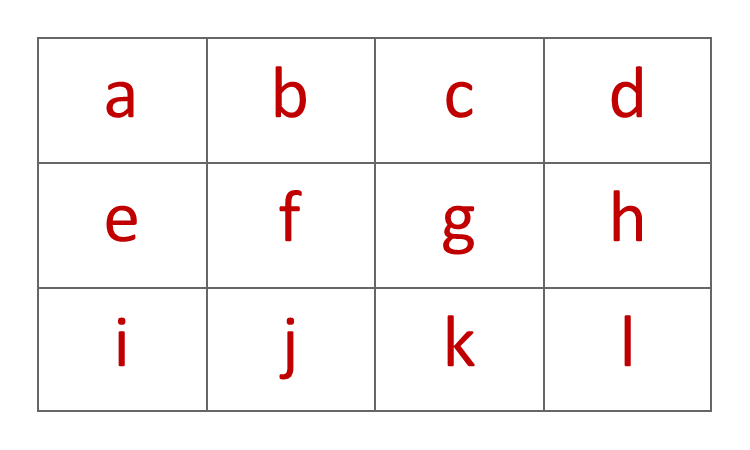
\includegraphics[scale=0.6]{../figures/2DConvExample(a)}
	\caption{Input Activations, $x^{(l-1)}$}
	\end{subfigure}	
	\begin{subfigure}{0.45\textwidth}
	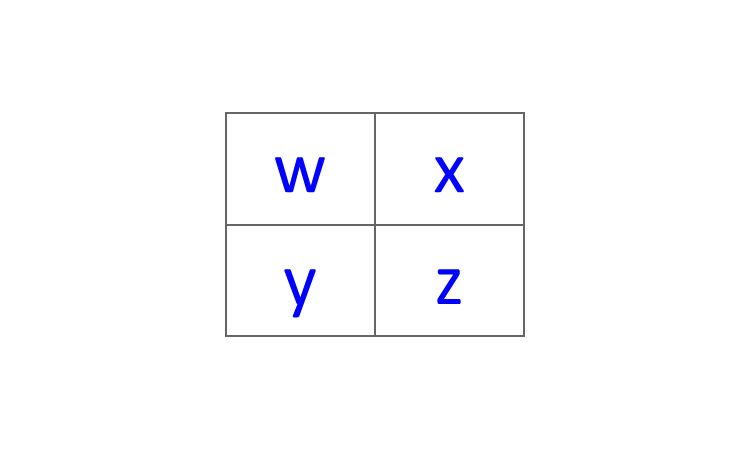
\includegraphics[scale=0.6]{../figures/2DConvExample(b)}
	\caption{Convolution Filter, $W^{(l)}_k$}
	\end{subfigure}	
	\begin{subfigure}{0.9\textwidth}
	\centering
	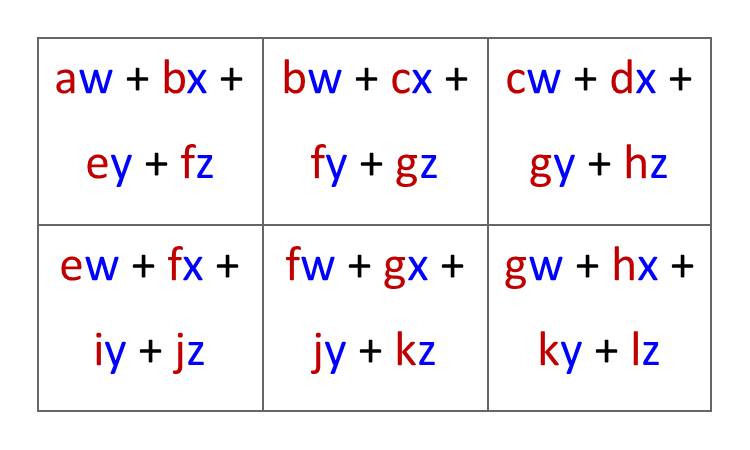
\includegraphics[scale=0.6]{../figures/2DConvExample(c)}
	\caption{Convolution Result, $x^{(l)}_k$}
	\end{subfigure}	
\end{center}
\caption{The result of convolving an input (a) with an filter map (b) is a new set of activations (c). This Image was adapted from Goodfellow, pg. 325 \cite{Goodfellow}}
\label{fig-2DConvExample}
\end{figure}
Note that formal implementations include a bias vector and an activation function.

\paragraph*{}For 2D convolution layer $(l)$, given input $x^{(l-1)}$, we compute the activations of the $k$-th filter $x^{(l)}_{k}$ using feature map $W^{(l)}_k$ and bias neuron $b^{(l)}_k$ as \cite{Goodfellow}:
\begin{equation}
\label{eqn-ConvFeedForward}
x^{(l)}_k(i,j) = \sigma^{(l)}\bigg[ b^{(l)}_k +  \sum_{u=0}^{m-1} \sum_{v=0}^{n-1} W^{(l)}_k(i,j) x^{(l-1)}_k(i - u,j - v) \bigg]
\end{equation}
This operation repeats for each of the $K$ feature maps. Each maps has it's own $n \times m$ weighting matrix and appropriately shaped bias .

\paragraph*{}The convolution layers allows for several advantages over the dense layer. Among these are (i) \textit{sparse-connectivity}: not every single activation (pixel) is connect to every single output pixel, so it is more computationally efficient, (ii) \textit{positional invariance}: key features can be identified regardless of where they are in the layer, and (iii.) \textit{Automatic feature detection} as the training process will update the filters to identify dominant features in the data without human instruction \cite{Geron,Goodfellow,Loy}. Below we detail what the "Call" method for a 2-dimensional convolutional neural network may look like. Compare this procedure with Eq. (\ref{eqn-ConvFeedForward}).

\begin{algorithm}[H]
\caption{Typical "Call" method for a 2-Dimensional Convolutional layer in a neural network that uses $K$ filters, of $m \times n$ kernels, with an assumed stride size of $1 \times 1$. This example shows the computation over a single input $x^{(l-1)}$ but a practical implementation should include mini-batches of samples.}
\label{alg-CallConv2D}

\begin{algorithmic}
\REQUIRE $x^{(l-1)} \leftarrow$ Input activations shaped into $(M \times N)$ matrix
\REQUIRE $K \leftarrow$ The number of filters (feature maps) to be used.
\REQUIRE $\sigma \leftarrow$ Activation function for this layer
\REQUIRE $W \leftarrow$ array of weight kernels containing $W_k, k \in [0,1,...,K-1]$ each shaped $m \times n$ \\
\REQUIRE $b \leftarrow$ a $(1 \times K)$ vector of bias values, $b_k, k \in [0,...,k-1]$ \\

\FOR {Each feature map, $k \in [0,1,2,...,K-2,K-1]$}
	\item Evaluate linear activation values by computing the 2D convolution-product of 
	$W_{k}$ and $x^{(l-1)}_{k}$:\\
	\item $z_{k}[i,j] \leftarrow b_{k} + 
	\sum_{i=0}^{N-1}\sum_{j=0}^{M-1} W_{k}[u,v] x^{(l-1)}_{k}[u-i,v-j]$ \\
	\item Evaluate output activation values by applying the activation function to each element in the linear activation matrix $z$:\\
	$x^{(l)}_{k}[i,j] \leftarrow \sigma\big[ z_{k}[i,j] \big]$ \\
\ENDFOR

Store both activation arrays for back-propagation. Return the output activations from each of the $K$ filters:\\
\RETURN $x^{(l)}$

\end{algorithmic}
\end{algorithm}

% ================================

\subsubsection{2-Dimensional Maximum Pooling Layer}
\label{subsubsec-2DPool}

\paragraph*{}A Maximum Pooling layers returns the maximum neuron activation in a two-dimensional group of neurons. In the case of 2D Max Pooling, we choose a kernel size to be $m \times n$, similar to the convolution layer, and extract the maximum value in each window, while stepping along according to a chosen stride size \cite{Loy,Goodfellow}. Consider an input like in Fig. (\ref{fig-2DConvExample}a). Using the $2 \times 2$ kernel on the $3 \times 4$ input, each box would then contain the maximum value of the input activations. We detail this in Fig. (\ref{fig-2DMaxPool}):
\begin{figure}[H]
	\begin{subfigure}{0.45\textwidth}
	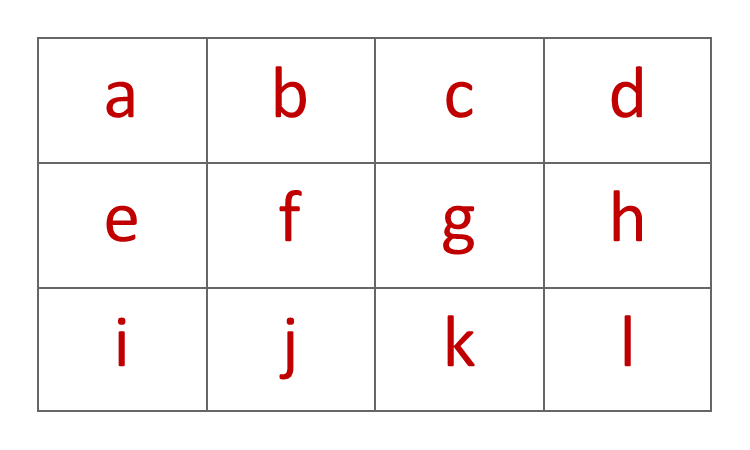
\includegraphics[scale=0.6]{../figures/2DConvExample(a)}
	\caption{Input Activations, $x^{(l-1)}$}
	\end{subfigure}
	\begin{subfigure}{0.45\textwidth}
	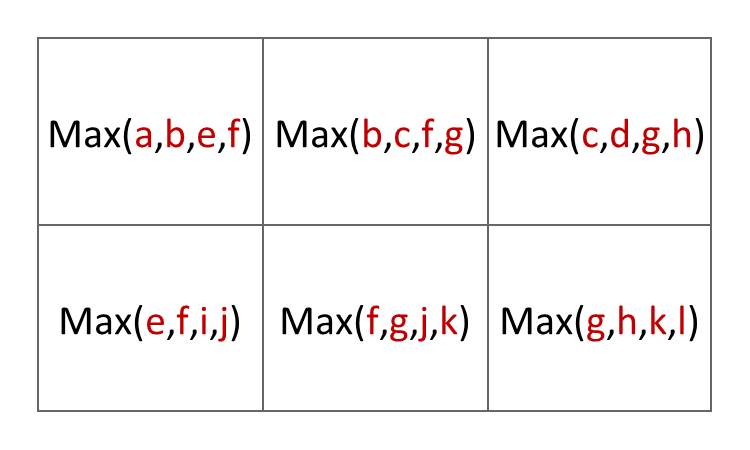
\includegraphics[scale=0.6]{../figures/2DConvExample(d)}
	\caption{Output Activations, $x^{(l)}$}
	\end{subfigure}
\caption{The result of 2D maximum-pooling an input array. This image was adapted from Loy, pg. 126 \cite{Loy}}
\label{fig-2DMaxPool}
\end{figure} 

\paragraph*{}Pooling layers, such as maximum pooling, average pooling, or similar are typically placed after a layer or a set of layers of convolution \cite{Loy}. The purpose of this arrangement is to reduce the number of activations by selecting only the largest valus, thereby dropping the width of the model and ensuring only features with large activation values are preserved \cite{Geron,Loy,Goodfellow}. This layer "non-trainable" because it does not use any weights or transformations, only a fixed procedure that cannot be updated. Below, we detail what the "Call" method for a 2D maximum pooling layer might look like.

\begin{algorithm}[H]
\caption{Typical "Call" method for a 2-Dimensional Maximum Pooling layer in a neural network. We assume 2D input, but a practical implementation may include the need to loop over a high dimensional structure. For simplicity, we assume a stride size of $1 \times 1$. This example shows the computation over a single input $x^{(l-1)}$ but a practical implementation should include mini-batches of samples.}
\label{alg-CallPool2D}

\begin{algorithmic}
\REQUIRE $x^{(l-1)} \leftarrow$ Input activations shaped into $(M \times N)$ matrix
\REQUIRE $m \times n \leftarrow$ Pool height and width
\REQUIRE $P \leftarrow$ A temporary pool array of shape $m \times n $ to hold local activations

\FOR {$i \in [0,1,...,M-2,M-1$}
	\FOR {$j \in [0,1,...,N-2,N-1$}
		\item Collect local activations in $P$, zero pad if necessary
		\item $P = x^{(l-1)}[i:i+m,j:j+n]$
		\item Find maximum value in $P$, and add to output
		\item $x^{(l)}[i,j] = \max\big( P \big)$
	\ENDFOR
\ENDFOR

Store the activation array for back-propagation, and return it
\RETURN $x^{(l)}$

\end{algorithmic}
\end{algorithm}

% ================================

\subsubsection{1-Dimensional Flattening Layer}
\label{subsubsec-1DFlatten}

\paragraph*{}A flattening layer is used to compress an array with two or more dimensions down into a single dimension. For a flattening layer $(l)$, multidimensional activations in layer $(l-1)$ are rearranged down into an array such that each sample contains only one axis. Note that a batch of samples will still be two-dimensional. This is not like projecting the data into a lower dimension, but rather is the reorganization of values into an array of a row of column array. We can use function notation to express this for a single sample as:
\begin{equation}
\label{eqn-FlattenFunction}
f^{(l)} : x^{(l-1)} \in \mathbb{R}^{(M \times N \times ....)} \rightarrow
x^{(l)} \in \mathbb{R}^{(MN...\times 1)}
\end{equation}
The numerical value of each activation is left unchanged. For a layer with activation shape$M \times N$, the resulting activations are reshaped into $MN \times 1$ as shown in Eq.(\ref{eqn-FlattenFunction}).

\paragraph*{}Flattening Layer are most commonly used to prepare activations for entry into dense layer or series of dense layers. For example, an image may contain two or three dimension, and convolution over it will return two or three dimensional activations per sample. Each sample must be compressed into one dimensions so that it can be processed by dense layers. This layer also is "non-trainable" because it does no use any weights or transformations, only a fixed procedure.

% ================================

\subsubsection{1-Dimensional Concatenation Layer}
\label{subsubsec-1DConcat}

\paragraph*{}The 1-Dimensional Concatenation Layer, also called 1D-Concat layer takes separate arrays of activations and combines them into a single array, while preserving the dimensionality of the sample. Consider the layer activations $\vec{a}^{(l-1)}$ and $\vec{b}^{(l-1)}$ with shapes  $1 \times \alpha$ and $1 \times \beta$ respectively. They are the outputs of two different layers:
\begin{equation}
\vec{a}^{(l-1)} = \big[ a_{0},  a_{1}, ... ,  a_{\alpha-1} \big]
\text{\hspace{1cm} and \hspace{1cm}}
\vec{b}^{(l-1)} = \big[ b_{0},  b_{1}, ... ,  b_{\beta-1} \big]
\end{equation}
The result of the concatenation is a new 1D-array, $\vec{c}^{(l)}$ with size $1 \times \alpha + \beta$:
\begin{equation}
\vec{c}^{(l)} = \big[ a_{0},  a_{1}, ... ,  a_{\alpha-1}, b_{0},  b_{1}, ... ,  b_{\beta-1} \big]
\end{equation}

\paragraph*{}We can denote this for $n$ arrays with function notation:
\begin{equation}
\label{eqn-ConcatenationFunction}
f^{(l)} : x^{(l-1)}_{a} \in \mathbb{R}^{(1 \times \alpha)} , x^{(l-1)}_{b} \in \mathbb{R}^{(1 \times \beta)} , ....  \rightarrow
x^{(l)}_{z} \in \mathbb{R}^{(1 \times \alpha + \beta + ...)}
\end{equation}
The concatenation layer is used to combine activations from two different layers into a single new layer. In this case of the model used in the project, we combine the outputs that result from the convolution branch and the perceptron branch to produce an single aggregated output. This process is detailed further in section (\ref{subsec-Architecture}). This layer also "non-trainable" because it does no use any weights or transformations, only a fixed procedure.

% ================================================================

\subsection{Activation Functions Used in Network Layers}
\label{sec-ActivationFunctions}

\paragraph*{}Activation functions are an important factor in the behavior of neural networks \cite{Geron}. For the convolution or dense layer, activation functions make up the second transformation step as in Eq. (\ref{eqn-elementActivation}) which allows for the neural network to produce non-linear decisions. In this section, we detail the activation functions used in this classification model.

\subsubsection{Rectified Linear Unit}

\paragraph*{}The Rectified Linear Unit (ReLU) activation function acts element-wise on the activations in a given layer. If the activation of a neurons is non-negative, the value is untouched, otherwise a $0$ is returned. For an input activation array $x$, ReLU is defined by:
\begin{equation}
\label{eqn-ReLU}
\text{ReLU}\big[x\big] = \max\big(0,x\big) = \left\{
\begin{array}{ll}
    x & \text{if\hspace{0.5cm}} x > 0 \\
    0 & \text{otherwise}
\end{array} 
\right.
\end{equation}
We provide a visualization of the function in Fig. (\ref{fig-ReLU}).
\begin{figure}[H]
\begin{center}
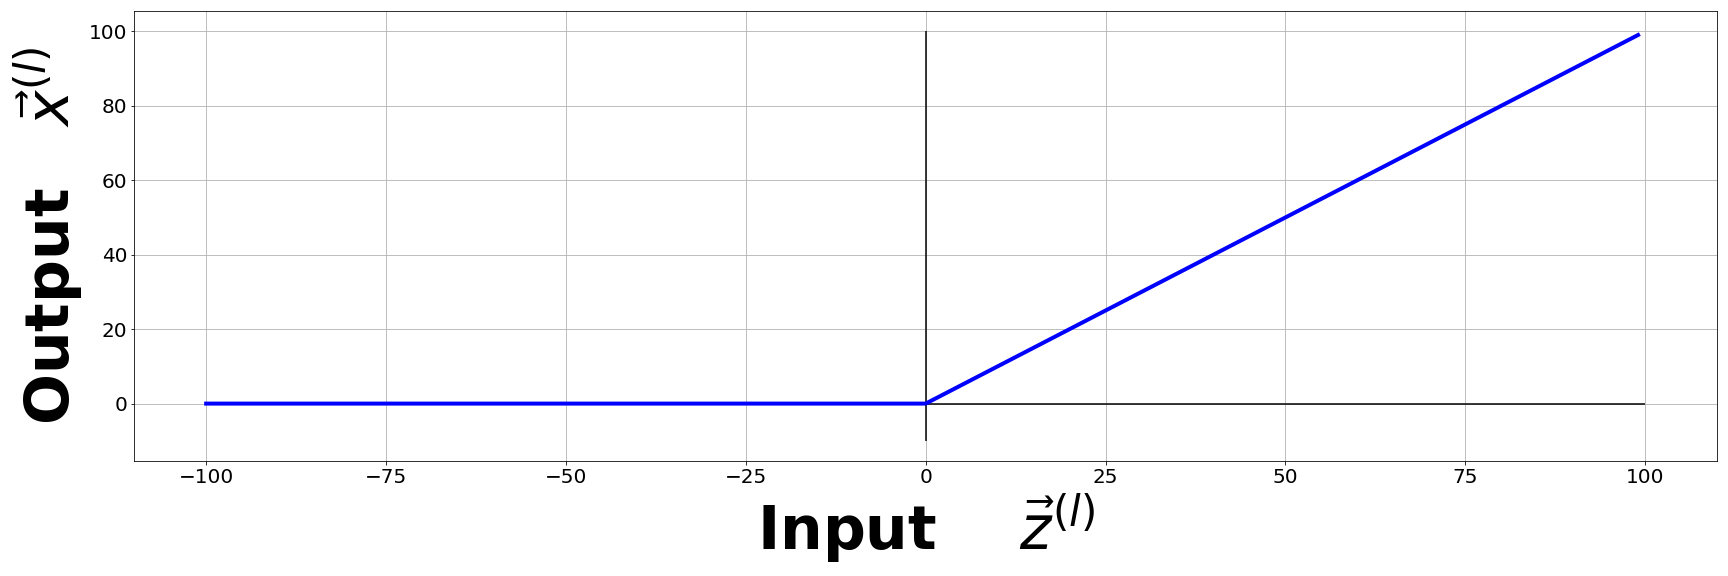
\includegraphics[scale=0.25]{../Figures/RectifiedLinearUnit}
\end{center}
\caption{Rectifed Linear Unit (ReLU) activation function}
\label{fig-ReLU}
\end{figure}
For our chosen architecture, ReLU is applied to the activations in every single Convolution layer and Dense Layer, with the exception of the output dense layer.

% ================================

\subsubsection{Softmax}
\label{subsubsec-Softmax}

\paragraph*{}The softmax activation function is commonly used in the output layer of a multi-class classification network, such as the one we implement \cite{Geron,Loy}. When softmax acts on a vector of activations, the result a non-negative output vector with an $L_1$ norm of $1$ \cite{Geron,Goodfellow,Virtanen}. The $i$-th element in a softmax activation function is given by:
\begin{equation}
\label{eqn-Softmax}
\text{Softmax}\big[ x \big]_{i} = \frac{e^{x_i}}{\sum_{j}e^{x_j}}
\end{equation}

\paragraph*{}If Eq.(\ref{eqn-Softmax}) returns a vector of the form: $[ 0.75 , 0.25]$, we interpret this as a sample having a $75\%$ chance of belonging to class $0$ and a $25\%$ change of belonging to class $1$. This tool is particularly useful is we are interested in determining the predictive confidence of a network. For example, if some if the two largest values in the output vector are very similar in magnitude, then the classifier is likely having a hard time differentiating between those two classes.

% ================================================================

\subsection{Training The Model}
\label{subsec-Training}

\paragraph*{}A neural network's purpose is to produce a function $F^*$ that approximates an unknown function $F$, using a set of parameters, $\Theta$. The model must have a procedure for updating the parameters in $\Theta$ to allow for a reasonably close approximation of $F$ \cite{Goodfellow}. To better understand this, we turn to Tom Mitchell's explanation of a learning algorithm \cite{Mitchell}:
\begin{quote}
A computer program is said to learn from experience $E$ with respect to some class of tasks $T$ and performance measure $P$, if it's performance at tasks in $T$, as measured by $P$, improves with experience $E$.
\end{quote}
Without any direct human intervention, a model must update itself to improve it's performance at a give task as new information is presented to it. To do this, the model must be constructed with a training procedure in mind. 

\paragraph*{}We consider the set of parameters $\Theta$ as the set of values within each trainable layer's weighting matrix and bias vector such that:
\begin{equation}
\label{eqn-Theta}
\Theta = \big\{
W^{(0)}, b^{(0)}, W^{(1)}, b^{(1)}, W^{(2)}, b^{(2)}, ... ,W^{(L-2)}, b^{(L-2)}, W^{(L-1)}, b^{(L-1)}
\big\}
\end{equation}
The arrays $W^{(l)}$and bias vectors $b^{(l)}$ are not trainable parameters themselves, but the the floating-point entries within them are the values that can be adjusted. Each element in this set may contain hundreds or thousands of parameters, so we represent these indirectly as parameters within their respective layers. We choose this representation of $\Theta$ for notation simplicity. Note that not all layers have trainable parameters, and activations functions themselves are not trainable, but fixed functions. Modern neural networks can contain upwards of hundreds of thousands,or even millions of elements in $\Theta$ making a neural network a functions that exist is a very high dimensional parameter-space \cite{Geron,Goodfellow,Levine}. For the network that we have designed in this project, there are roughly $33,000$ parameters across $20$ layers. In this sections we motivate and explore how the we can update the parameters in $\Theta$ as to train the neural network.

% ================================

\subsubsection{The Cost Function}

\paragraph*{}Suppose we pass a training sample into the neural network. This sample is represented by the feature-vector $x^{(0)}$, with an expected outcome given by the one-hot-encoded vector $y$.  After the network finishes processing, it's output activations, given by the vector $x^{(L-1)}$, also noted as $y^*$, represents the prediction for the class label. For a reasonably trained model, we expect the vector $y^*$ to be "similar" to $y$, indicating that model has made a a reasonable prediction with the given input values. Alternatively, for an untrained network, $y^*$ is not likely to be "similar" to $y$ at all, indicating that the model has made a poor prediction with the given input.

\paragraph*{}To quantify the difference between the model's prediction, $y^*$ and the expected output, $y$, we introduce a \textit{cost function}, $J(y^*,y)$ \cite{Goodfellow,James}. The cost function, also called a \textit{loss} or \textit{objective} function, compares $y^*$ and $y$ to return a single scalar value which measures the quality of the prediction. A high cost value indicates a \textit{poor} prediction, and a low cost indicates a reasonable prediction. We can generalize this idea to consider that we want a trained neural network to produce a consistently low cost function value across samples in a data set.

\paragraph*{}The cost function itself, $J(y^*,y)$ can take many forms and is often dependent on particular task or data set provided \cite{James}. For this $k$-classes classification task, we choose to use the \textit{Categorical Crossentropy} (CXE) cost function. For a sample labeled by the one-hot-encoded vector $y$ and corresponding prediction vector $y^*$, the CXE objective value for a single sample is given by \cite{Bishop,Goodfellow,Virtanen}:
\begin{equation}
\label{eqn-CXELoss}
\text{CXE}\big[ y , y^* \big] = - \sum_{i=0}^{k-1} y_i \ln(y^*_i) 
\end{equation}
Thus, the average loss over a mini-batch of $b$ samples is given:
\begin{equation}
\label{eqn-CXELossAvg}
\big\langle \text{CXE}\big[ y , y^* \big]\big\rangle = 
- \frac{1}{b}\sum_{n=0}^{b-1}\sum_{i=0}^{k-1} y_i^{(n)} \ln(y^{*(n)}_i) 
\end{equation}

\paragraph*{}Suppose that a given sample belongs to class $j$ in a $k$-classes classifier. Since the label vector, $y$ is one-hot-encoded, all entries are zero except $y_{j} = 1$.
\begin{equation}
y = \big[y_0,y_1, ... , y_{j} , ..., y_{k-1} \big]^T  = 
\big[0,0, ... , 1 , ...,0 \big]^T
\end{equation}
Thus the sum in Eq. (\ref{eqn-CXELoss}) contains mostly zero terms, with the only exception at index $j$, where we have $y_j\ln(y^*_j) = \ln(y^*_j)$. Since the vector $y^*$ has been subject to the softmax activation function, we must have $y^*_j \in [0,1]$. This means that taking the natural log of this value returns a negative number. Multiplying that by $-1$ returns a high loss when the activation of $y^*_j << 1$ and a low cost when $y^*_j \approx 1$. We visualize this relationship for a single sample in Fig. (\ref{fig-CXELoss}):

\begin{figure}[H]
\begin{center}
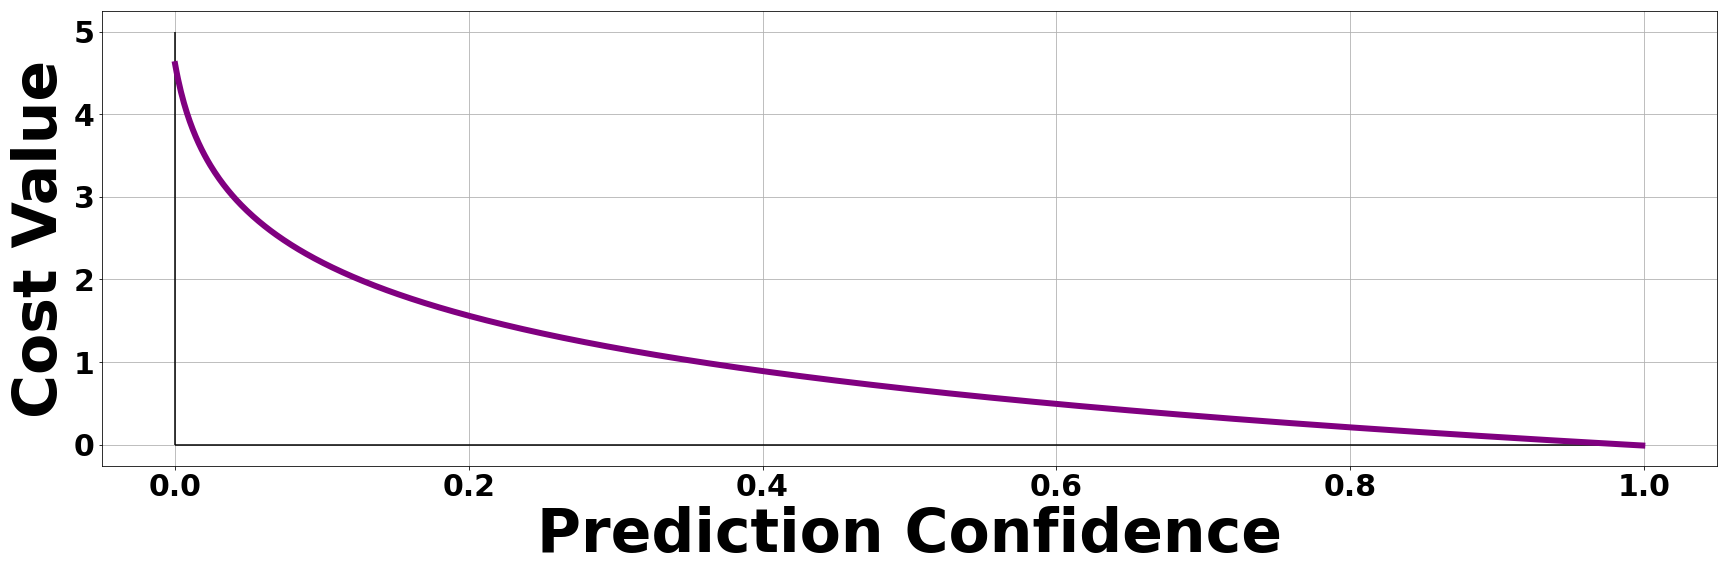
\includegraphics[scale=0.25]{../Figures/CXELoss}
\end{center}
\caption{Plot of how $y^*_{j} \in [0,1]$ affects the output values of the CXE cost function}
\label{fig-CXELoss}
\end{figure}

\paragraph*{}By optimizing the parameters $\Theta$ in the network model, we allow for the output of a consistently low cost function to be produced across all samples in the data set. When a model produces consistently low cost values across new unseen samples, this means that $y^* \approx y$ and we consider this to be a \textit{trained} or \textit{fitted} neural network \cite{Goodfellow,Loy,Mitchell}.

% ================================

\subsubsection{Gradient Based Learning}

\paragraph*{}We have developed a method for quantifying the difference between a given output $y^*$ and an expected output $y$ with the inclusion of a cost function. The process of training the model is to choose the parameters in $\Theta$ that allows for consistently low values of the cost function. We then treat the training process of training a neural network as a high dimensional \textit{optimization} problem. A neural network uses \textit{indirect optimization}, which contrasts from pure optimization. Deep Learning expert Ian Goodfellow describes the difference \cite{Goodfellow}:
\begin{quote}
In most learning scenarios, we care about some performance measure $P$,... We reduce a different cost function, $J(\theta)$ in the hope that doing so will also improve $P$.
\end{quote}
By choosing an appropriate cost function, and selecting the parameters $\Theta$ that minimize the average cost over a data set, we assert that $y^* \approx y$, but can only assume that doing so minimizes classification error and improves the performance metrics.

\paragraph*{}The cost value of a sample is dependent on the relationship between training labels $y$ and the network output $y^*$. The output is given by the final layer activation $x^{(L-1)}$, which in turn are produced by the previous layer and so forth, as demonstrated in Eq. (\ref{eqn-altLayerFunction}), This recursive nature combined with the dimensionality of the parameter object $\Theta$ makes an analytical solution to the optimization impractical \cite{Geron,Goodfellow,James}. We instead optimize the cost function with a numerical iterative method called \textit{gradient descent} \cite{Loy}. 

\paragraph*{}We can reduce the cost given a set of parameters, $J(\Theta)$, by repeatedly stepping each element in $\Theta$. We step each element acording to the direction and manitude of each element in a gradient vector, $\nabla_\Theta J$, which is the gradient of the cost function with respect to each parameter in $\Theta$. We express the gradient of $J$ with respect to the parameters in $\Theta$ as:
\begin{equation}
\label{eqn-CostGradient}
\nabla_{\Theta}\big[ J \big] = 
\Big[ 	\frac{\partial J}{\partial W^{(0)}}, \frac{\partial J}{\partial b^{(0)}}, 
		\frac{\partial J}{\partial W^{(1)}}, \frac{\partial J}{\partial b^{(1)}}, \hdots ,
		\frac{\partial J}{\partial W^{(L-1)}}, \frac{\partial J}{\partial b^{(L-1)}} \Big]^T
\end{equation}
Where $\frac{\partial J}{\partial W^{(l)}}$ is taking the partial derivative of each element $W_{i,j}$ in the $W^{(l)}$ matrix, and preserves the shape. While there may only be $20$ or so layers, the gradient vector actually has one element for every trainable parameter in the $\Theta$ object. This means that for our network, the gradient vector contains upwards of $33,000$ elements. We again choose to group these elements by their parent structure for ease of notation.

\paragraph*{}Due to the nested composition of the network output in Eq. (\ref{eqn-FunctionChain}), and subsequently the cost itself, we must use the chain rule of calculus to work backwards through computational graph of the neural network to compute the partial derivative of $J$ with respect to each parameter in $\Theta$. The process of working backwards to compute each element in the gradient vector is called \textit{back-propagation} \cite{Geron,Goodfellow,Loy}. 



% ================================

\subsubsection{Back-Propagation}
\label{subsubsec-BackProp}

\paragraph*{}Recall our model of a neural network as a computational graph as in Eq. (\ref{eqn-FunctionGraph}). Each node of the graph is a layer that represents a mathematical function which takes the activation from the previous layer $x^{(l-1)}$ and transforms them into the activations of the current layer, as in Eq. (\ref{eqn-altLayerFunction}). Additionally, we recall that each layer with trainable parameters is made up of two steps which produce linear activations such as in Eq. (\ref{eqn-LinearTransform}) and non-linear activations, as in Eq. (\ref{eqn-elementActivation}). Therefore, to understand back propagation, it is helpful to examine the flow of information within each layer. Consider a simplified neural network model visualized in Fig. (\ref{fig-ComputationalGraph}). Note that we indicate the cost as $J(\Theta)$. This is alluding to the fact that $y^*$ is ultimately a function of the parameters in $\Theta$.

\paragraph*{}Raw information is presented as $x^{(0)}$ at the top of the figure, and and output is returned as $x^{(L-1)}$ at the bottom. (Recall $y^* = x^{(L-1)}$) Arrows represent the flow of information in the network. Because of the nested computation nature of the graph, we use the chain rule for partial derivatives to begin at the final output of the network and successively work our way forward to the entry layer. At each step, we compute the numerical derivative with respect to the parameters in each layer. This process is called \textit{back-propagation} \cite{Geron,Goodfellow}.

\begin{figure}[H]
\begin{center}
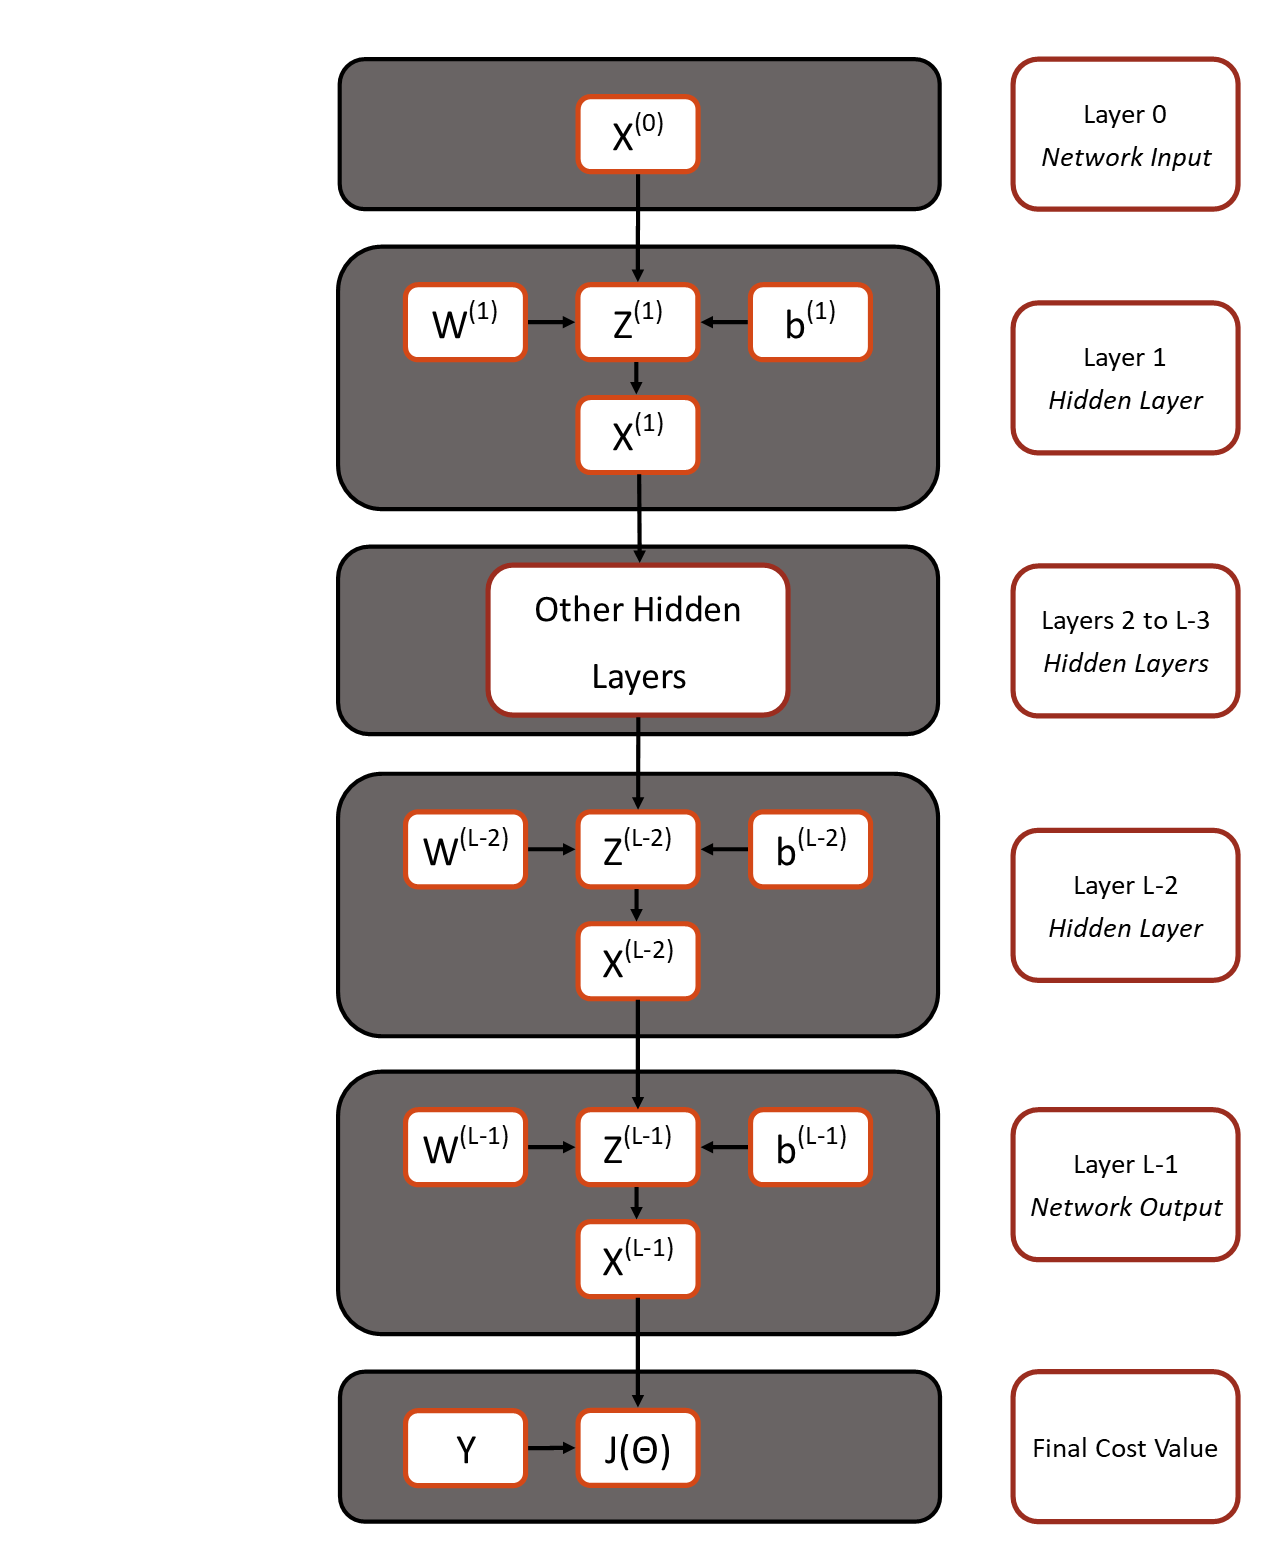
\includegraphics[scale=0.8]{../Figures/LayerGraph}
\end{center}
\caption{A visual representation of a simplified neural network as a computational graph}
\label{fig-ComputationalGraph}
\end{figure}

\paragraph*{}Suppose we wish to compute the elements of $\frac{\partial J}{\partial W^{(L-1)}}$ and $\frac{\partial J}{\partial b^{(L-1)}}$ for the gradient vector. The flow of information in Fig. (\ref{fig-ComputationalGraph}) indicates that we cannot directly evaluate the derivative because the cost $J$, is a function $x^{(L-1)}$, which is a function of $z^{(L-1)}$, which is a function of elements in $W^{(L-1)}$. Thus, we have:
\begin{equation}
\frac{\partial J}{\partial W^{(L-1)}} = \frac{\partial}{\partial W^{(L-1)}}
\Bigg[ J \bigg\{ x^{(L-1)} \Big[ z^{(L-1)}  \big\{ W^{(L-1)} 
\big\} \Big] \bigg\} \Bigg]
\end{equation}
The evaluation of the derivative of a composite function requires use of the chain rule of multivariate calculus. We represent this symbolically as:
\begin{equation}
\label{eqn-dWL1}
\frac{\partial J}{\partial W^{(L-1)}} = 
\frac{\partial J}{\partial x^{(L-1)}}\frac{\partial x^{(L-1)}}{\partial z^{(L-1)}}\frac{\partial z^{(L-1)}}{\partial W^{(L-1)}}
\end{equation}
Similarly, the partial derivative of the cost with respect to the bias array can be formulated as:
\begin{equation}
\label{eqn-dbL1}
\frac{\partial J}{\partial b^{(L-1)}} = 
\frac{\partial J}{\partial x^{(L-1)}}\frac{\partial x^{(L-1)}}{\partial z^{(L-1)}}\frac{\partial z^{(L-1)}}{\partial b^{(L-1)}}
\end{equation}

\paragraph*{}For the categorical cross entropy cost function, we can evaluate $\partial J / \partial x^{(L-1)}$ over a single sample that belongs to class $i$ as:
\begin{equation}
\label{eqn-CXELossDeriv}
\frac{\partial J}{\partial x^{(L-1)}} = \frac{\partial J}{\partial y^*} =
\frac{\partial}{\partial y^*}\Big[ -y \ln (y^*) \Big] = -\frac{y}{y^*_i + \delta} = -\frac{1}{y^*_i + \delta}
\end{equation}
We often introduce $\delta \approx 10^{-8}$ to prevent possible division by $0$ errors. The value $\partial x^{(L-1)} / \partial z^{(L-1)}$ can be found by differentiating Eq. (\ref{eqn-elementActivation}) with respect to the input activations.
\begin{equation}
\frac{\partial x^{(L-1)}}{\partial z^{(L-1)}} = \sigma^{'(l)} \big[ z^{(L-1)} \big]
\end{equation}
For a dense layer as in section (\ref{subsubsec-DenseLayer}) or a 2D-convolution layer as in section (\ref{subsubsec-Conv2DLayer}) $\partial z^{(L-1)} / \partial W^{(L-1)}$ is given by the derivative of Eq. (\ref{eqn-LinearTransform}) or Eq. (\ref{eqn-LinearTransform2}) with respect to $W^{(l)}$:
\begin{equation}
\frac{\partial z^{(L-1)}}{\partial W^{(L-1)}} = 
\frac{\partial}{W^{(L-1)}}\Big[ W^{(L-1)}x^{(L-2)} + b^{(L-1)}\Big] = x^{(L-2)}
\end{equation}
\begin{equation}
\frac{\partial z^{(L-1)}}{\partial W^{(L-1)}} = 
\frac{\partial}{W^{(L-1)}}\Big[ \big( W^{(L-1)} * x^{(L-2)} \big) + b^{(L-1)}\Big] = x^{(L-2)}
\end{equation}
Finally, differentiating with respect to the bias array: $\partial z^{(L-1)} / \partial b^{(L-1)}$, we have:
\begin{equation}
\frac{\partial z^{(L-1)}}{\partial b^{(L-1)}} = \frac{\partial}{W^{(L-1)}}\Big[ W^{(L-1)}x^{(L-2)} + b^{(L-1)}\Big] = 1
\end{equation}

\paragraph*{}Suppose we then wish to compute the elements of $\frac{\partial J}{\partial W^{(l)}}$ and $\frac{\partial J}{\partial b^{(l)}}$ for any layer $(l)$. Using the same graph from Fig. (\ref{fig-ComputationalGraph}), we can follow the chain of information to derive an expression for the similar to Eq. (\ref{eqn-dWL1}) and Eq. (\ref{eqn-dbL1}) for each layer $(l)$ in the nueral network. In general, we can state that:
\begin{equation}
\label{eqn-dWGeneral}
\nabla_{W^{(l)}}J = \frac{\partial J}{\partial W^{(l)}} = 
\frac{\partial J}{\partial x^{(l)}}\odot \partial\sigma^{(l)}[ z^{(l)} ] \cdot x^{(l-1)}
\end{equation}
And
\begin{equation}
\label{eqn-dbGeneral}
\nabla_{b^{(l)}}J = \frac{\partial J}{\partial b^{(l)}} = 
\frac{\partial J}{\partial x^{(l)}}\odot \partial\sigma^{(l)}[ z^{(l)} ]
\end{equation}
Where $z^{(l)}$ are the linear activations defined in Eq. (\ref{eqn-LinearTransform}) and Eq. (\ref{eqn-LinearTransform2}). Note that each $z^{(l)}$ and $x^{(l)}$ are typically stored in memory during the forward pass in Alg. (\ref{alg-FeedForward}) to prevent the need to recompute them \cite{Geron2,Goodfellow}.


\begin{algorithm}[H]
\caption{Backwards propagation system, in a standard densely connected deep neural network. Each iteration in the \textit{for-loop} computes the gradient of the cost function $J$ with respect to the weight and bias arrays in a given layer $(l)$. Each element in those arrays $dW$ and $db$ is the discrete gradient of the cost due to that parameter. A practical application of this algorithm should include batches of samples instead of a single sample and a regularizing function at each step.}
\label{alg-BackProp}

\begin{algorithmic}
\REQUIRE Cost/Objective function $J$.
\REQUIRE Set of Layer functions $f^{(i)}$. Each one contains a weighting array $W^{(i)}$, a bias array $b^{(i)}$, and activation function $\sigma^{(i)}$, the activation function derivative, $\sigma^{'(i)}$. In all cases, $i \in \{0,1,....,L-1\}$
\REQUIRE Set of linear and non-linear activation arrays $z^{(i)}$ and $x^{(i)}$.

Execute forward pass in algorithm (\ref{alg-FeedForward}) and compute the gradient of the cost with respect to the final layer activations \\
$dx \leftarrow \nabla_{(y^*)}J(y,y^*)$ \\
Initialize $\nabla J$ as output object, should have same shape as $\Theta$

\FOR {$l \in [L-1,L-2,...,2,1]$}
	\item Compute gradient w.r.t pre-nonlinear activation portion of layer function
	\item $dx^{(l)} \leftarrow \nabla_{Z^{(l)}}J = dx^{(l)} \odot \partial\sigma^{(l)}[ Z^{(l)} ]$
	\item Compute gradient w.r.t weighting and bias elements
	\item $db \leftarrow \nabla_{b^{(l)}}J = dx^{(l)}$
	\item $dW \leftarrow \nabla_{W^{(l)}}J = dx^{(l)} \cdot X^{(l-1)}$

	\item Add $db$ and $dW$ steps to $\nabla J$ object
	\item $\nabla J = \nabla J .Add(dW,db)$
\ENDFOR

\item Return gradient w.r.t to each parameter in $\Theta$
\RETURN $\nabla J$

\end{algorithmic}
\end{algorithm}

\paragraph*{}After (i) computing the gradient, we can scale it by a desired learning rate $\alpha$ wich controls the size of the gradient step in each component, and (ii) add the gradient vector element-wise to the existing elements in $\Theta$ object. By repeating steps (i) and (ii) in succession, we gradually drive the cost function to produces consistently lower and lower values across a data set \cite{Geron}. This is called \textit{gradient descent} and is the basis for many optimization algorithms. Let $\bar{J}$ be the average cost over a batch of $b$ samples. We show the general update rule on iteration $(i)$ for gradient based learning in Eq. (\ref{eqn-GradientLearning}) \cite{Geron,Goodfellow}.
\begin{equation}
\label{eqn-GradientLearning}
\Theta^{(i)} = \Theta^{(i-1)} + (-\alpha) \nabla_{\Theta} \bar{J}
\end{equation}
Where $\Theta^{(i)}$ will give the set of new, updated parameters of the network. Note that for Eq. (\ref{eqn-GradientLearning}), all operations are applied element-wise.

% ================================

\subsubsection{The Optimizer}
\label{subsubsec-Optimizer}

\paragraph*{}An optimizer is the algorithm or procedure that is used by a machine learning model to perform the optimization task to reduce the cost value after reciveing each new training sample. Regression models may often used a \textit{mean-squared error} cost function which can often be solved analytically, while high dimensional neural networks, such as the one used in this project, outlined in section (\ref{subsec-Architecture}), can only up updated iteratively \cite{Goodfellow,James,Loy}. We use a variation of gradient descent much like the one in Eq. (\ref{eqn-GradientLearning}). A standard stochastic gradient-based or batch gradient descent learning algorithm can be fast, but are often prone errors such as vanishing or exploding gradients \cite{Geron,Goodfellow,Loy}. To combat this, model must often implement an optimizer that is more stable, and robust in it's ability to drive the cost function to a successively lower value.

\paragraph*{}For this project, we employ an \textit{Adaptive-Moments} optimizer, also called \textit{ADAM} for short. This is a powerful algorithm that uses an adaptive learning rate and built-in momentum parameter. ADAM records and updates an exponentially decaying average of past gradients, $s^{(i)}$, and an exponentially decaying average of past squared gradients, $r^{(i)}$ in Eq. (\ref{eqn-ADAMupdate}) \cite{Geron}. This produces a far more aggressive optimizer at a higher computational cost than standard gradient descent \cite{Goodfellow}.

\paragraph*{}As the optimizer iterates through each step, the effect of past iterations will tend to "snowball". If the previous step was found to reduce the cost function by a large or small amount, the step size for the previous step will update accordingly. This enables to ADAM to overcome smaller discontinuities that may arise in the model's solution space \cite{Goodfellow}. For a given step $(i)$, The ADAM update is given:
\begin{equation}
\label{eqn-ADAMupdate}
\begin{split}
s^{(i)} &= \rho_1 s^{(i-1)} + (1 - \rho_1) \nabla_{\Theta} \bar{J}  \\
r^{(i)} &= \rho_2 r^{(i-1)} + (1 - \rho_2) \Big[ \nabla_{\Theta} \bar{J} \odot \nabla_{\Theta} \bar{J} \Big]  \\
s'^{(i)} &= \frac{s^{(i)}}{1-\rho_1^i} \\
r'^{(i)} &= \frac{r^{(i)}}{1-\rho_2^i} \\
\Theta^{(i)} &= \Theta^{(i-1)} + (-\alpha)\frac{s'^{(i)}}{\sqrt{r'^{(i)}}+\delta} \\
\end{split}
\end{equation}
Note that a superscript $(i)$ or $(i-1)$ gives an iteration index, while the superscript $i$ means to raise a value to the power of $i$. ADAM has experimentally shown to be a very powerful and robust optimizer useful for a wide range of tasks \cite{Goodfellow}. Because of the two decay constants $\rho_1$ and $\rho_2$, we can compound and accumulate the values of past gradients to continue to push the cost to lower and lower values, even if the magnitude of the gradient becomes very small \cite{Geron}. 

\begin{algorithm}[H]
\caption{Adaptive-Moments (ADAM) optimizer for a neural network. This algorithm is adapted from Goodfellow \cite{Goodfellow}}
\label{alg-ADAM}

\begin{algorithmic}
\REQUIRE Step size $\alpha$
\REQUIRE Small constant $\delta$ for numerical stabilization, usually about $10^{-7}$.
\REQUIRE Constants $\rho_1$, $\rho_2$ used track exponential decay rates, usually $0.9$ and $0.999$ respectively.
\REQUIRE Subroutine/function to compute gradient of cost function See Alg. (\ref{alg-BackProp})
\REQUIRE Mini-batch size, $m$
\REQUIRE Stopping criterion $S$

Initialize moment variables and iteration counter $s = 0$, $r = 0$, $i = 0$ \\

\WHILE {Stopping Criterion $S$ is \FALSE}
	\item Extract a mini-batch of $m$ samples from larger data set $X$. $[x^{(0)},x^{(1)},...,x^{(m-1)}]$ and corresponding target values 
	$[y^{(0)},y^{(1)},...,y^{(m-1)}]$.
	\item Compute numerical gradient estimate of each sample in batch. This can be done with standard back-propagation in algorithm (\ref{alg-BackProp}) and 			 	normalize by batch size $m$:
	\item $\nabla \bar{J} \leftarrow \frac{1}{m} \nabla_{\Theta} \Big[\sum_{n=1}^{m} J(y^{*(n)},y^{(n)}) \Big]$
	
	\item Compute first bias moment: $s \leftarrow \rho_1 s + (1 - \rho_1) \nabla \bar{J}$
	\item Compute second bias moment: $r \leftarrow \rho_2 r + (1 - \rho_2) \big( \nabla \bar{J} \odot \nabla \bar{J} \big)$
	\item First bias correction: $s' \leftarrow \frac{s}{1 - \rho_1^i}$
	\item Second bias correction: $r' \leftarrow \frac{r}{1 - \rho_2^i}$
	
	\item Compute And Apply update:	$\Delta \Theta \leftarrow (-\alpha) \frac{s'}{\sqrt{r'} + \delta}$
	\item $\Theta \leftarrow \Theta + \Delta \Theta$	
	\item Update Iteration number: $i \leftarrow i + 1$
\ENDWHILE

\end{algorithmic}
\end{algorithm}


% ================================================================

\subsection{Multimodal Architecture}
\label{subsec-Architecture}

\paragraph*{}In addition to choosing a strong set of features, and an appropriate optimizer for a classification task, it is also important to combine the predictors with a complementary network architecture. Since a neural network is a computational graph with each layer represented by a node, it can take on a nearly infinite number of different shapes and structures \cite{Goodfellow,Virtanen}. The structure of the network defines the composition of it's function, $F^*$ as in Eq.(\ref{eqn-FunctionGraph}), and thus affects it's performance in completing any given task \cite{Geron}. The layer structure of the neural network is referred to as it's \textit{architecture}, and define it's \textit{hypothesis - space} \cite{Goodfellow}. 

\paragraph*{}For this project, we have derived features that describe that audio file using two different \textit{modalities}. A modality is a method of describing and interpreting a sample of data \cite{Ngiam}. For example humans can be said to experience the world through five modalities - those being our cardinal senses of sight, hearing, taste, smell and touch. The sight and sound of a guitar are two very different ways of experiencing the same thing. One or the other is often enough to identify the guitar - but both together yield an even higher predictive confidence. Since modalities are \textit{different} by nature, we cannot simply combine them into a single object and present the neural network with it. We must account for the difference by providing two distinct input layers.  Modalities of seeing and hearing are captured by two different senses but ultimately processed by the same brain to produce a single prediction.

\paragraph*{}We can carry this idea over by producing a \textit{multimodal} neural network that accepts two different forms of input for each sample. One input is an $N' \times k$ spectrogram matrix, explored in section (\ref{subsec-Spectrogram}) and the other input is a $1 \times p$ feature vector explored in section (\ref{subsec-TimeFeatures}) and section (\ref{subsec-FreqFeatures}). The spectrogram acts to provide an energy distribution of a signal as a function of frequency and time, while the feature vector provides qualities in a more list-like fashion. This type of supervised learning is referred to as \textit{multi-representation learning}, and we detail a conceptual diagram of the architecture in Fig. (\ref{fig-NetworkArchitecture}) \cite{Li,Ngiam}.

\begin{figure}[H]
\begin{center}
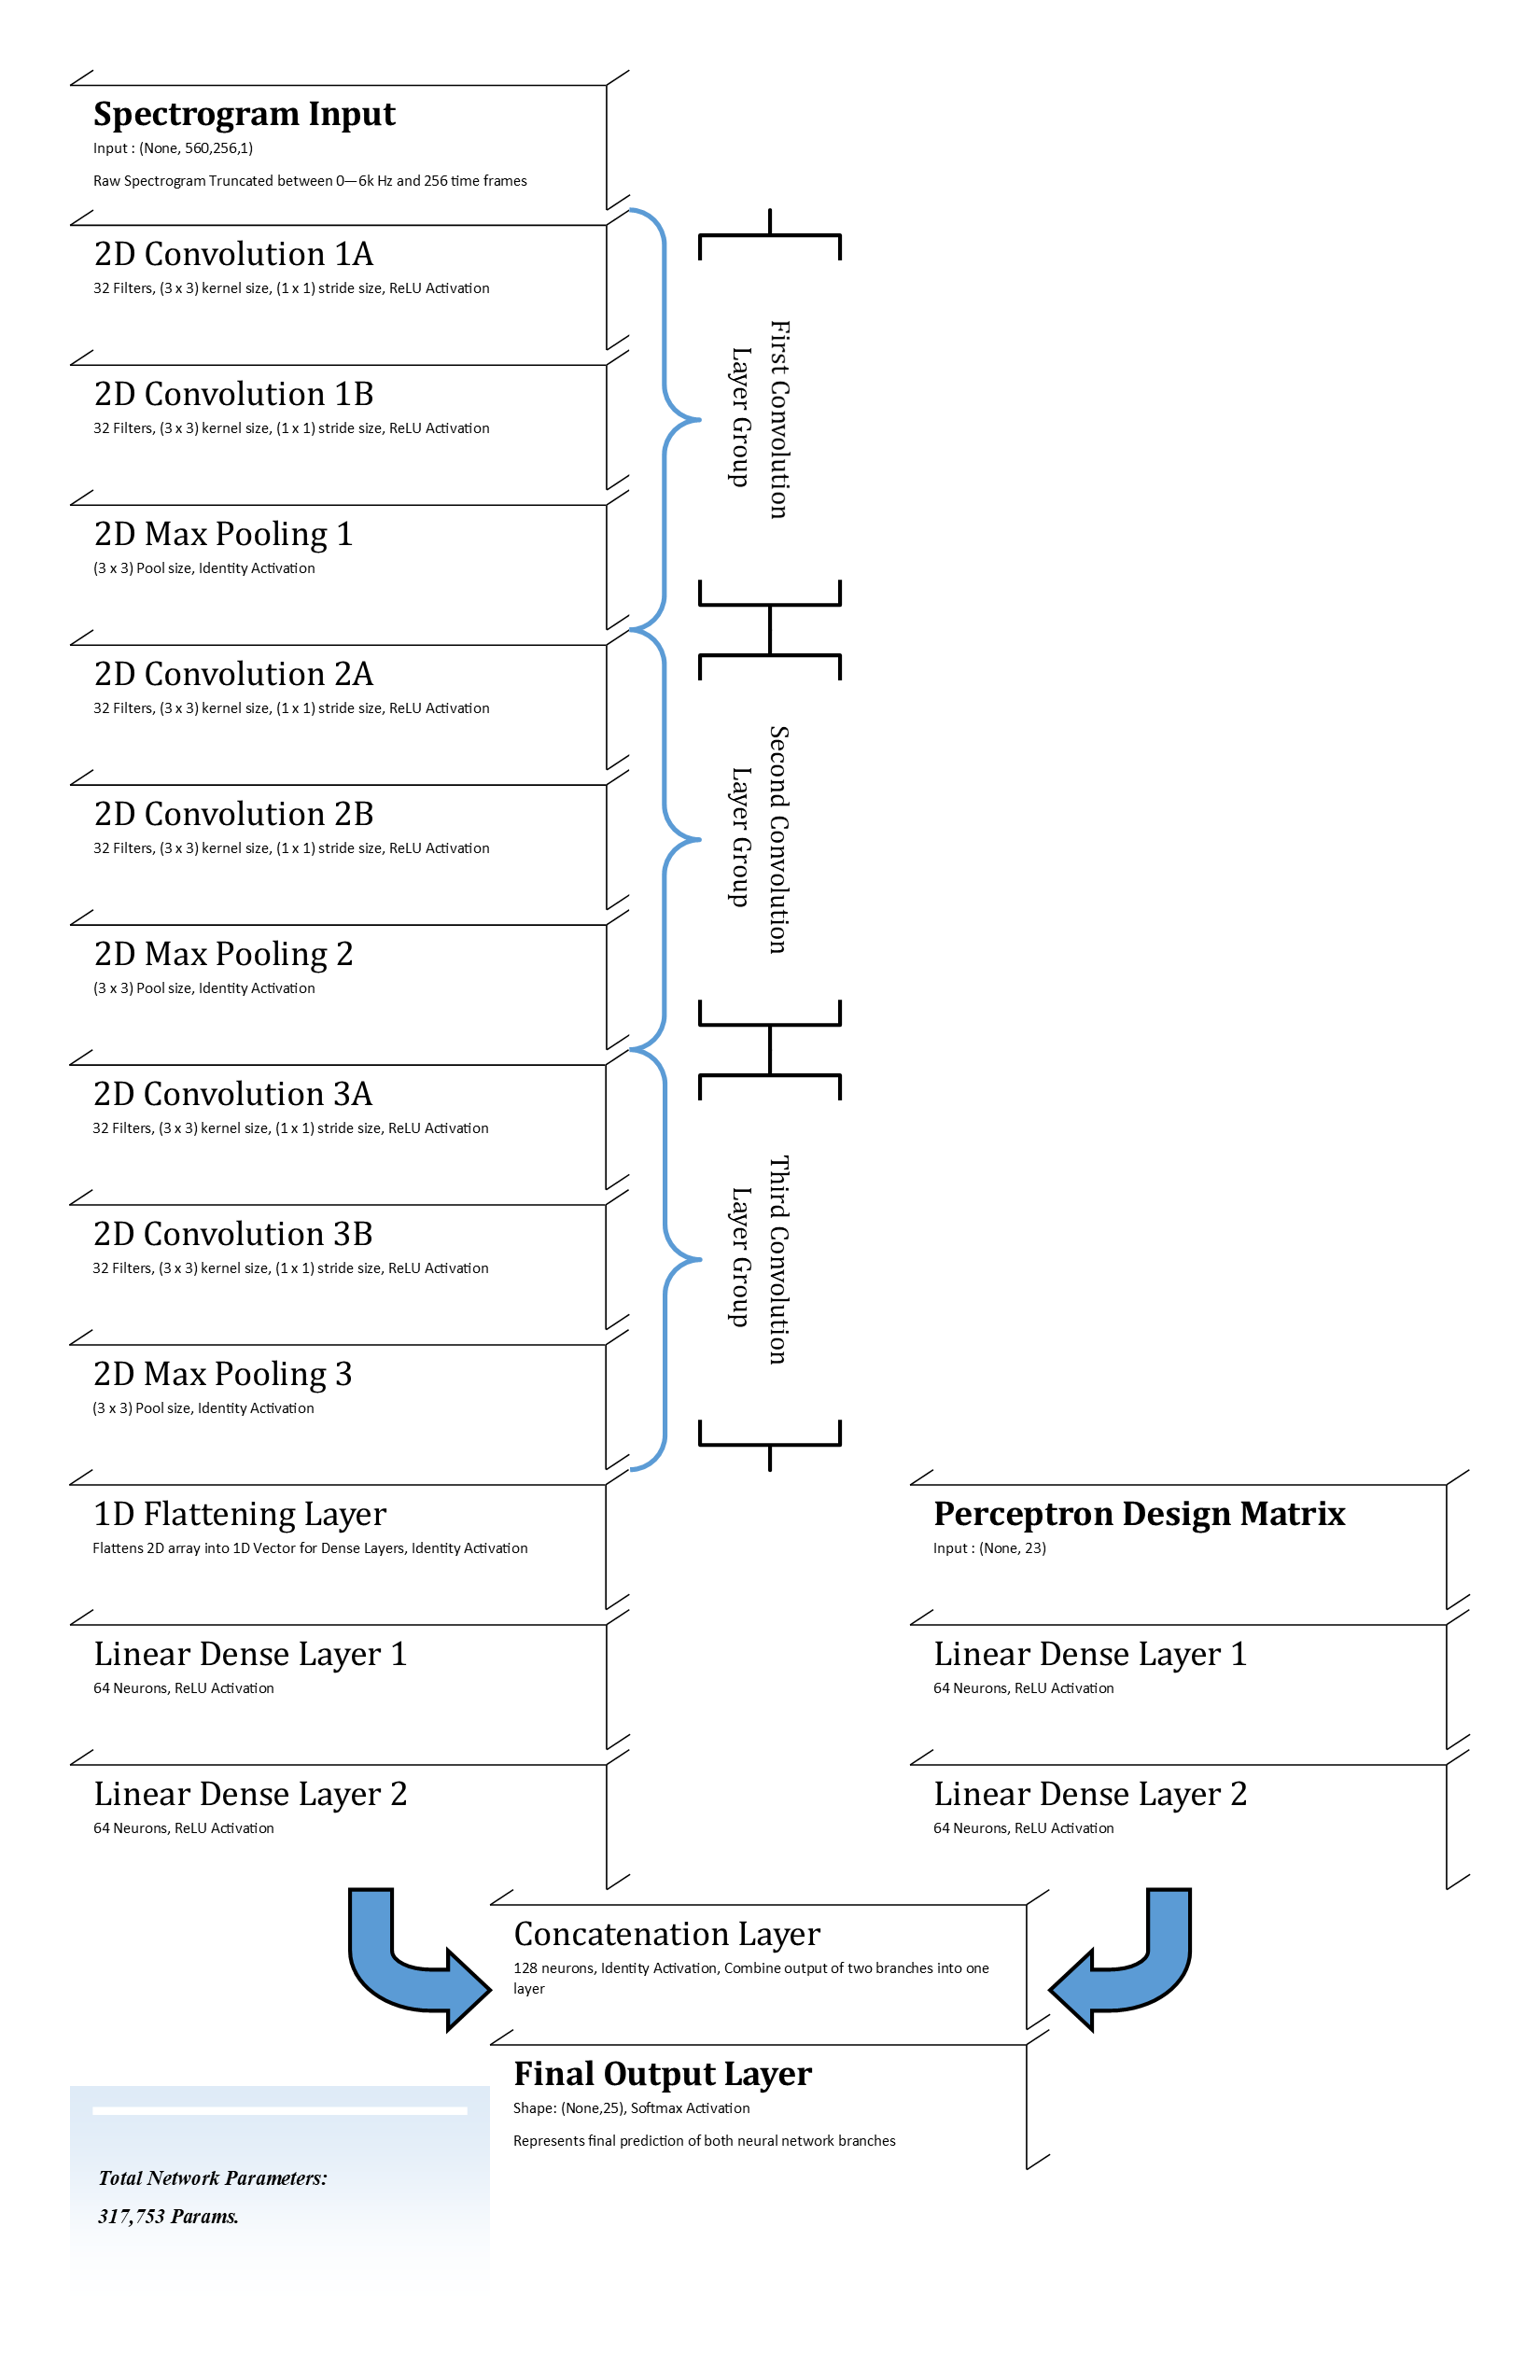
\includegraphics[scale=0.75]{../Figures/NeuralNetworkArchitecture}
\end{center}
\caption{The implemented multimodal architecture of the audio file classification neural network. The left branch process an image-like input, and the right branch processes a vector-like input. The activations are then merged, and then a single output vector is produced}
\label{fig-NetworkArchitecture}
\end{figure}



% ================================

\subsubsection{The Convolution Branch}

\paragraph*{}The convolution branch is pictured on the left side of Fig. (\ref{fig-NetworkArchitecture}), and is an implementation of a \textit{convolutional neural network} (CNN). It processes a spectrogram, which is a representation of a waveform, or signal as an energy distributions over \textit{time} and \textit{frequency} \cite{White,Olson,Khan}. The input layer of this branch accepts a 4-Dimensional array. The axes, in order of indexing, represents (i) the size of the \textit{mini-batch} of samples, (ii) the pixel height of each sample, (iii) the pixel wifth of each sample, and (iv) the number of channels in the image. For this model, we have selected to use $64$ samples per batch, $558$ pixels in height, $256$ pixels in width, and $1$ gray-scale channel. We denote the 4D shape of the design matrix for this branch as:
\begin{equation}
\label{eqn-shapeX1}
X_1 \in \mathbb{R}^{(64 \times 558 \times 256 \times 1)}
\end{equation}
Any other shape will be rejected, and an error is raised.

\paragraph*{}The input layer holds the input activations, $X_1$, which is a collection of $64$ spectrograms. The output of the the input layer is passed into the first of three \textit{Convolution Layer Groups}. These layer groups are inspired from the \textit{Visual Geometry Group-16 Neural Network} architecture \cite{Goodfellow,Loy}. Each convolution layer group is composed of three individual layers: 
\begin{enumerate}
\item A 2-Dimensional Convolution layer, $32$ filters, $3 \times 3$ kernel, $1 \times 1$ step size, ReLU activation function,
\item A 2-Dimensional Convolution layer, $32$ filters, $3 \times 3$ kernel, $1 \times 1$ step size, ReLU activation function,
\item A 2-Dimensional Maximum Pooling layer, $3 \times 3$ pooling size, Identity activation function
\end{enumerate}  
The convolution layers iterate over the middle two axes of the data, see section (\ref{subsubsec-Conv2DLayer}). Physically, this allows us to search through the frequency and time axes to detect dominant features or shapes.

\paragraph*{}By grouping layers in this structure, we use convolution to reduce the number of features, and then the pooling layer to extract only the largest activations of the remaining values. This drastically reduces the width of each layer before passing the activations down, and ensures that only the pertinent characteristic shapes are preserved and passed into the next layer set for processing. This also allows for positional invariance in features. Regardless of where in frequency or time a feature is detected, the moving kernel will still allow it to be found \cite{Goodfellow,Loy}.

% ================

\subsubsection{The Perceptron Branch}

\paragraph*{}The perceptron branch is pictured on the right side of Fig. (\ref{fig-NetworkArchitecture}) and is an implementation of a \textit{multilayer percepton neural network} (MLP). Rather than accept an image-like input, the perception simply takes a $p$-dimensional vector-like input of properties that are derived from the audio file. We call these properties \textit{features} or \textit{predictors} \cite{Geron,Khan,Serizel}. Details on the natures and selections of these $p$ elements are found in section (\ref{subsec-TimeFeatures}) and section (\ref{subsec-FreqFeatures}).

\paragraph*{}The input layer of the perceptron accepts a 2-Dimensional array. The axes, in order of indexing, represent (i) the size of the \textit{mini-batch} of samples, (ii) the number of features for each sample. We use the same model hyper-parameter of $b = 64$ samples per batch, and have developed $p = 24$ unique classification features that have been derived from time-space and frequency-space representations of the audio file data. We can denote the 2D shape if the input object into this branch as:
\begin{equation}
\label{eqn-shapeX2}
X_2 \in \mathbb{R}^{(64 \times 24)}
\end{equation}
This 2D array is referred to as a \textit{design matrix} \cite{James,Loy}. Any other shape will be rejected by the model, and an error is raised.

\paragraph*{}In perceptron models, the scaling of the design matrix is vital to classification performance. A design matrix is scaled by taking all samples in a column (a particular feature from each class), subtracting the average, and then scaling it such that it has unit variance \cite{Geron,James}. This ensures that no one feature dominates the performance of the model and that layer activations do not get saturated to extremes as data progresses through the network. This operation was implemented through the \textit{scikit-learn} Python package \cite{Sklearn}.

% ================

\subsubsection{The Final Output Branch}

\paragraph*{}The last layer in each of the two branches is a ReLU-activated Dense layer containing 64 neurons, represented by a $64$ - dimensional vector. We combine these model layers by using a \textit{concatenation layer} to fuse the arrays together, such that each sample is given by a $128$-dimensional vector. This vector is then transformed into the final dense layer, which uses the softmax activation, and encodes the joint predictions based on contributions of both model branches. In section (\ref{sec-Results}) we explore how the predictive power of the network changes when examining the performance of each individual branch compared to the hybrid model.

% ================================================================
% ================================================================

\newpage
\section{Properties of Musical Instruments}
\label{sec-Instruments}

\paragraph*{}As discussed in section (\ref{sec-TheNeuralNetwork}), performance quality of a neural network is greatly dependent on the properties of the chosen features \cite{Virtanen,Liu}. To ensure that the classifier model performs adequately and consistently, we must choose these features to have high variance between classes, and low variance within each class. This enables a neural network to development clear decision boundaries between each unique class \cite{James,Serizel}. To develop this set of features, we explore the physical and mechanical properties of musical instruments and the sounds that they create.

\paragraph*{}Since computer algorithms such are neural networks are built to handle exclusively quantitative information, we must ensure that each property can be represented by a numerical quantity \cite{Geron,Levine}. Where a human would use qualitative adjectives such as \textit{bright} or \textit{harsh} or \textit{percussive} to describe sound, computers require a numerical descriptor instead. The goal of this section is to develop the attributes of sound that enable us to describe a sound wave in a quantitative and compact way. Thus we use values that can be expressed as numbers such as \textit{amplitude envelopes}, \textit{frequency spectra}, or \textit{formant structure}. For this section, we represent waveforms as \textit{spectrograms} to capture the time-space and frequency-space development of energy simultaneously. We motivate and describe the production of a spectrogram in section (\ref{subsec-Spectrogram}).

\paragraph*{}We have assembled training data samples than can be grouped into $37$ classes of unique sources listed below:

\begin{figure}[H]
\begin{center}
\begin{tabular}{||c|c|c| |c|c|c||}
\hline
\textbf{Class Index} & \textbf{Class Name} & \textbf{Counts} & \textbf{Class Index} & \textbf{Class Name} & \textbf{Counts} \\
\hline \hline
$0$ & Alto Flute & $72$ 			& $20$ & Marimba & $364$ \\ \hline
$1$ & Alto Saxophone & $128$ 		& $21$ & Oboe & $666$  \\ \hline
$2$ & Banjo & $74$ 					& $22$ & Sawtooth Wave & $200$ \\ \hline
$3$ & Bass & $1060$ 				& $23$ & Tenor Saxophone & $732$ \\ \hline
$4$ & Bass Clarinet & $1036$ 		& $24$ & Sine Wave & $200$ \\ \hline

$5$ & Bass Flute & $76$ 			& $25$ & Soprano Saxophone & $128$\\ \hline
$6$ & Bassoon & $800$ 				& $26$ & Square Wave & $200$ \\ \hline
$7$ & Bass Trombone & $54$ 			& $27$ & Tenor Trombone & $66$ \\ \hline
$8$ & $B\flat$ Clarinet & $938$ 	& $28$ & Triangle Wave & $200$ \\ \hline
$9$ & Bells & $164$ 				& $29$ & Trombone & $831$ \\ \hline

$10$ & Violoncello & $1079$ 		& $30$ & $B\flat$ Trumpet & $627$ \\ \hline
$11$ & Contrabassoon & $710$ 		& $31$ & Tuba & $1046$ \\ \hline
$12$ & Crotale & $50$ 				& $32$ & Vibraphone & $334$ \\ \hline
$13$ & $E\flat$ Clarinet & $78$ 	& $33$ & Viola & $1173$ \\ \hline
$14$ & English Horn & $1382$ 		& $34$ & Violin & $787$ \\ \hline

$15$ & Flute & $1032$ 				& $35$ & Whitenoise & $200$ \\ \hline
$16$ & Guitar & $106$ 				& $36$ & Xylophone & $176$ \\ \hline
$17$ & Hihat & $10$ 				& $37$ & & \\ \hline
$18$ & French Horn & $740$ 			& $38$ & & \\ \hline
$19$ & Mandolin & $364$ 			& $39$ & & \\ \hline

\end{tabular}
\end{center}
\caption{Instruments categories used in the classification task. Note that the network uses only integers given by "Class index" to identify sources. The string "Class Name" is kept for human readability}
\label{fig-ClassList}
\end{figure}

\paragraph*{}Rather than explore each class individually, we can examine the properties of groupings of musical instruments by using the \textit{Hornbostel-Sachs} organization system developed by  Erich M. von Hornbostel and Curt Sachs, and published in 1961 \cite{Hornbostel}. In this system, musical instruments or sound sources can be divided up into four broad categories based on the nature of the sound-producing material. These categories are (i) idiophones, (ii) membranophones, (iii) chordophones, and (iv) aerophones. In this section, we show how the physics of the source instrument influences some of our feature choices.

% ================================================================

\subsection{Idiophones}
\label{subsec-Idiophone}

\paragraph*{}An idiophone is an instrument that produces sound through the vibration of the full body of the object. This generally includes most percussive instruments excluding drums \cite{Hornbostel}. From the set of classes that we use, bells, crotales, Hi-hats, marimbas, vibraphones, and xylophones are all examples of idiophones. In each case, sound comes from the vibration of the object itself or some subset of the body. In the case of mallet percussion, the wood or metal keys vibrate when struck with a felt or yarn mallet. Sometimes the vibration is amplified by nearby air columns, but it is the vibration of the key itself where the sound originates from \cite{Olson}.

\paragraph*{}Idiophones in particular can be characterized by their \textit{transient response} \cite{White}. The transient response is the time-evolution response of the waveform in time, which we normally break into \textit{attack}, \textit{decay}, \textit{sustain}, and \textit{release}. For most idiophones, the system is struck once and left to a free or dampened vibration; which we can mathematically model as a rigid body reacting to an impulse \cite{Hunter,Olson}.

\begin{figure}[H]
	\begin{subfigure}[b]{0.45\textwidth}
	\centering
	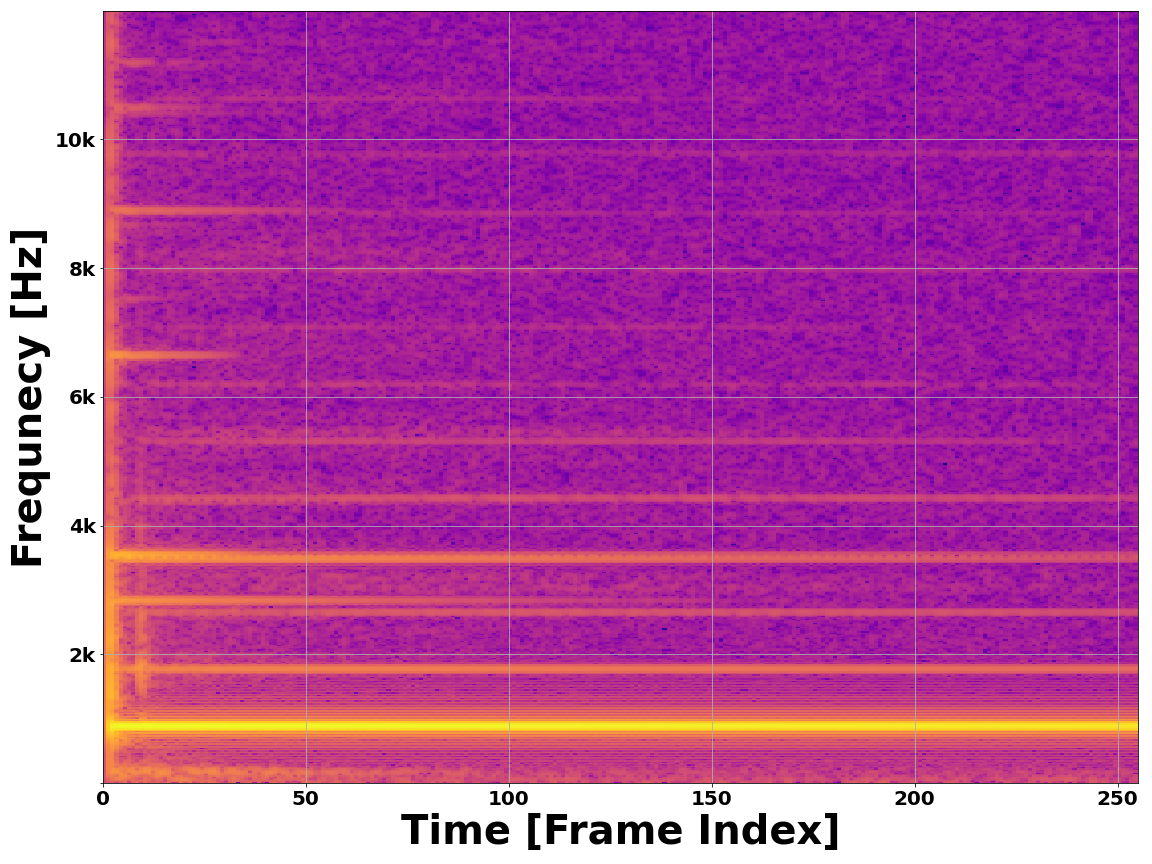
\includegraphics[scale=0.2]{../FiguresSpectrogram/Vibraphone-A5}
	\caption{Vibraphone playing $A5$}
	\end{subfigure}
	\hfill
	\begin{subfigure}[b]{0.45\textwidth}
	\centering
	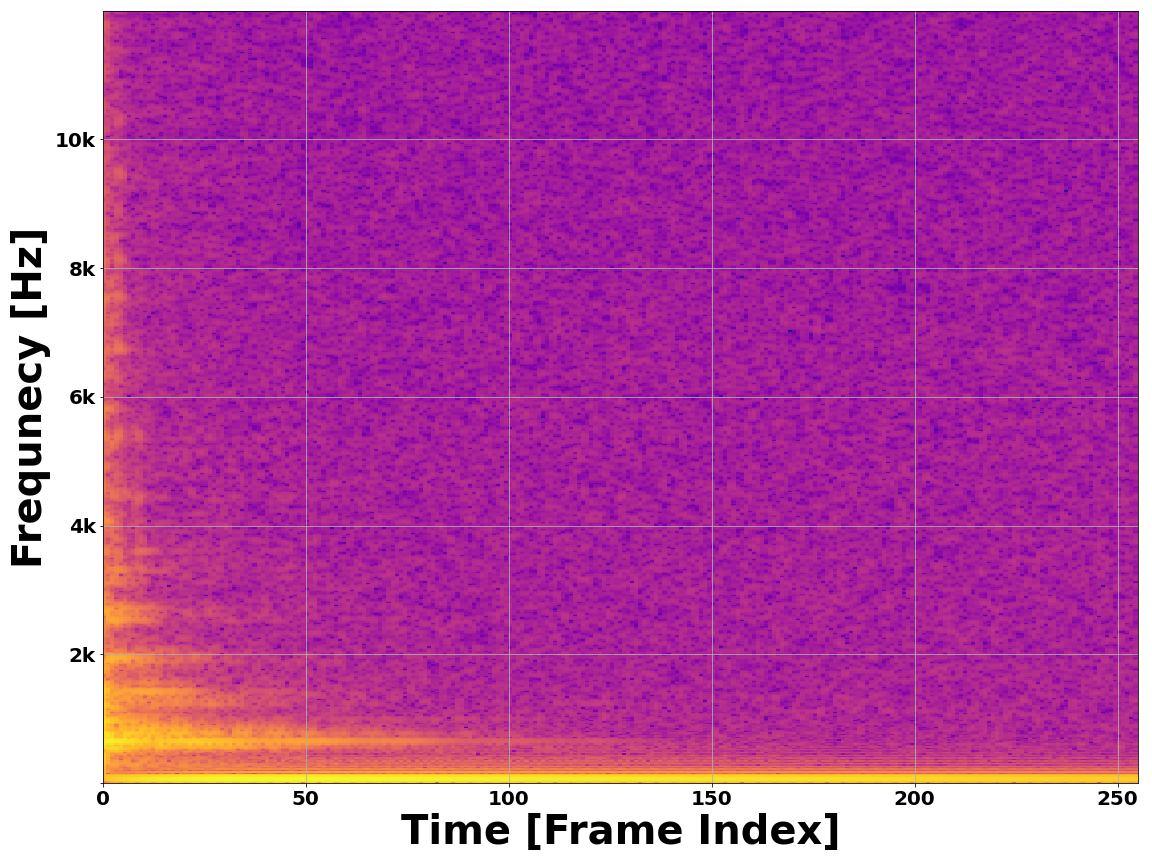
\includegraphics[scale=0.2]{../FiguresSpectrogram/Marimba-C2}
	\caption{Marimba playing $C2$}
	\end{subfigure}
\caption{Spectrograms from idiophone waveforms}
\label{fig-PropertiesIdiophones}
\end{figure}

\paragraph*{}From the spectrogram representation of idophone waveforms , we can see the majority of energy in the time domain is right at the start of the waveform. This is shown by the vertical bright yellow line at on the left side of each image in Fig. (\ref{fig-PropertiesIdiophones}). When an idiophone is struck, all of the energy for the vibration is delivered up front, and the amplitude can only decay. This gives the resulting transient a very short attack time, followed by a short decay, sustain, and often long release as the last of the energy dies out \cite{White}. While other instruments such as plucked strings like guitars show similar response, this is a very important property of many idiophones. Notice that the energy of the higher overtones die out very quickly in each spectrogram, and only the lowest pitch - the fundamental is preserved for much of the duration.

\paragraph*{}This property allows for us to distinguish idiophones from other instruments by an approximation of their amplitude envelope. For example, if we divide the time series waveform into $q$ distinct sections, and compute the RMS energy in each section, we should see a gradual decay of energy with time. More specifically, the energy in some section $q_i$ should be greater than the energy in any subsequent section $q_{i + n}, n \in \mathbb{Z}$. Having this property does not guarantee the source is an idiophone but can we can state within reason that most idiophones obey this behavior. In addition to the amplitude envelope, we can consider the distribution of time-space energy in the form of a single scalar quantity as the center of mass. If we treat the waveform as a 1D mass distribution, and compute the center of mass, we should see consistently low values because the largest values of amplitudes happen early on in the time-domain.

% ================================================================

\subsection{Membranophones}
\label{subsec-membranophones}

\paragraph*{}A membranophone is an instrument that produces sound through the vibration of a tight membrane \cite{Hornbostel}. This includes most drum-like instruments While none of the instruments that we classify are membranophones, they do exhibit some noteworthy properties that influence our feature for other instruments. Common examples include the tympani, the bass drum, or the kettle drum. Each of these instruments is composed of a large cylinder or bowl-like structure that serves as an amplifying cavity \cite{Olson,White}. Given that most membranophone instruments are played by striking the membrane with the hand or mallet, the amplitude envelope properties 

\paragraph*{}We model the tight elastic membrane very similarly as that of a tight elastic string, except in two dimensions \cite{White}. Unlike the chordophone section (\ref{subsec-chordophones}), the partials for the membrane are not related by integer multiples. This lack of harmonic structure leaves most membranophones to have a sort of "muddled" frequency spectrum where we see a more continuous distribution of constituent frequencies arise as opposed to clean integer related overtones \cite{White,Olson}. This partly why many membranophones have a much more "percussive" sound as opposed to performing any distinct note.

% ================================================================

\subsection{Chordophones}
\label{subsec-chordophones}

\paragraph*{}A chordophone is a musical instrument that produces sound through the vibration of strings that are stretched between two fixed points \cite{Hornbostel}. From our data set, banjos, basses, cellos, guitars, mandolins, violins, and violas are all examples of chordophones. We commonly model a chordophone as having a string of length $L$, with a constant linear mass density, $\mu$, subject to a tension force $F_T$. The string is flexible, and free to vibrate in a spatial single dimension, $x$. We describe the state of string over space and time with a function $U(x,t)$. The behavior of the string can be modeled by D'Alembert's 1-dimensional wave equation \cite{Haberman,Hunter,Taylor}:
\begin{equation}
\label{eqn-1DWaveEqn}
\frac{\partial^2 U}{\partial t^2} = v^2 \frac{\partial^2 U}{\partial x^2}
\end{equation}
Where $v$ is the wave propagation velocity, given by $\sqrt{\frac{F_T}{\mu}}$. D'Alembert's equation indicates that the acceleration of any point on a string is directly proportional to the rate of change of the slope of the string at that point \cite{Taylor}. 

\paragraph*{}Since the PDE is second order in time, we must also specify two initial conditions being the shape and the derivative of the shape at time $t = 0$.  \cite{Olson,White,Haberman}:
\begin{equation}
U(x,0) = f(x) 
	\text{\hspace*{2cm} and \hspace*{2cm}}
\frac{\partial U}{\partial t}(x,0) = g(x)
\end{equation}
Additionally, the string is fixed in place at both ends, with a nut at $x = 0$ and a bridge at $x = L$, which can be modeled by the boundary conditions
\begin{equation}
U(0,t) = 0 
	\text{\hspace*{2cm} and \hspace*{2cm}}
U(L,t) = 0 
\end{equation}
Depending on the exact nature of the source instrument, $f(x)$ and $g(x)$ can take on different forms. For example, for plucked stringed instruments, $f(x)$ may appear to be as triangle-like function, with a peak at some position $0 < x_0 < L$ where then string was struck. It is these initial conditions that allow for the drastically different timbres that arise in the wave forms \cite{Hunter}. Compare the spectrogram representation of a few stringed instruments in Fig. (\ref{fig-PropertiesChordophones}).
\begin{figure}[H]
	\begin{subfigure}{0.45\textwidth}
	\centering
	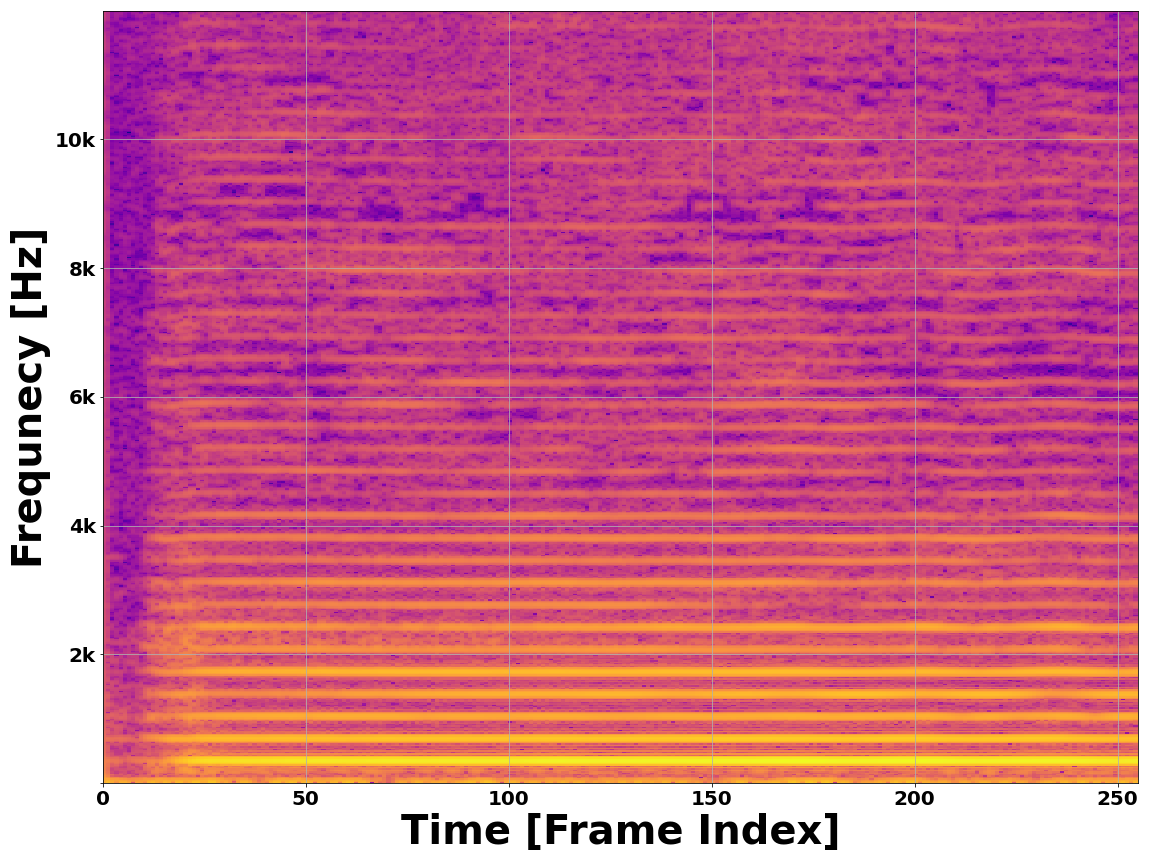
\includegraphics[scale=0.2]{../FiguresSpectrogram/CELLO-F4}
	\caption{Violoncello playing $F4$}
	\end{subfigure}
	\hfill
	\begin{subfigure}{0.45\textwidth}
	\centering
	\includegraphics[scale=0.2]{../FiguresSpectrogram/Guitar-B2}
	\caption{Guitar playing $B2$}
	\end{subfigure}
	
	\begin{subfigure}{0.45\textwidth}
	\centering
	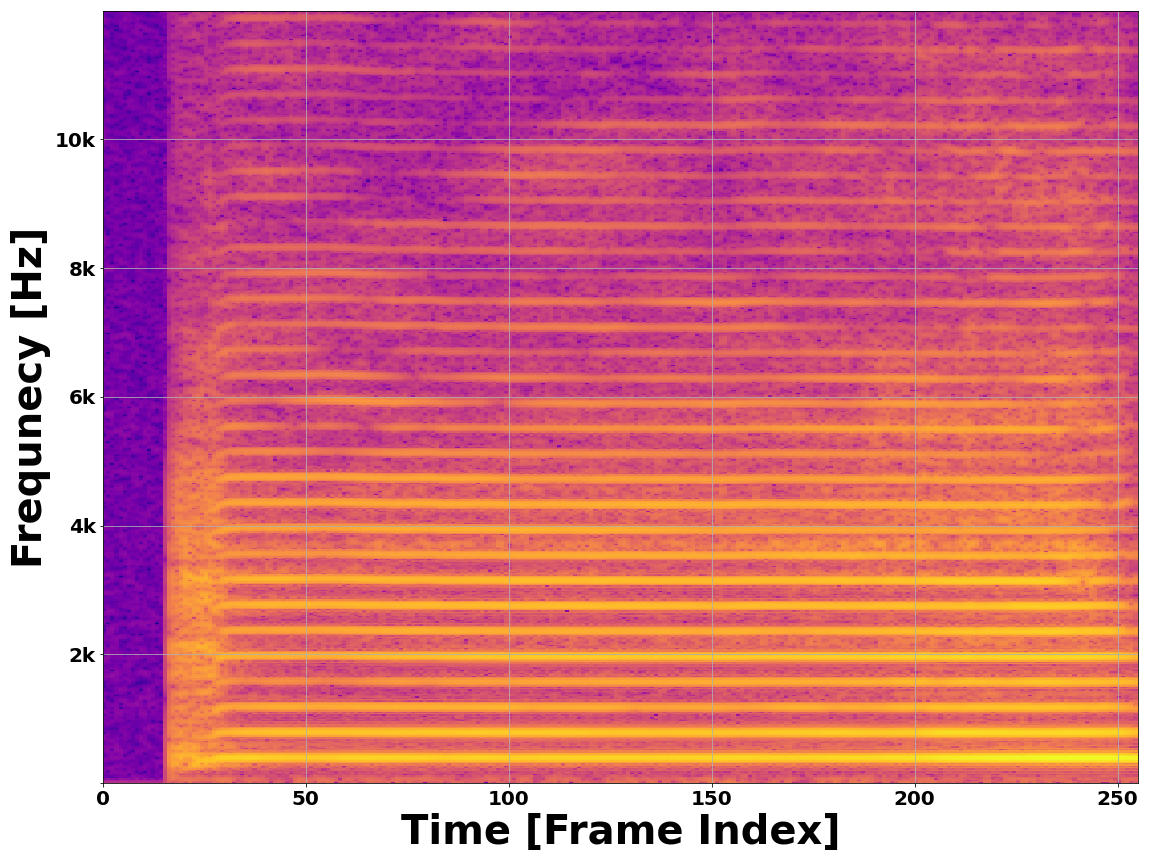
\includegraphics[scale=0.2]{../FiguresSpectrogram/Violin-G4}
	\caption{Violin playing $G4$}
	\end{subfigure}
	\hfill
	\begin{subfigure}{0.45\textwidth}
	\centering
	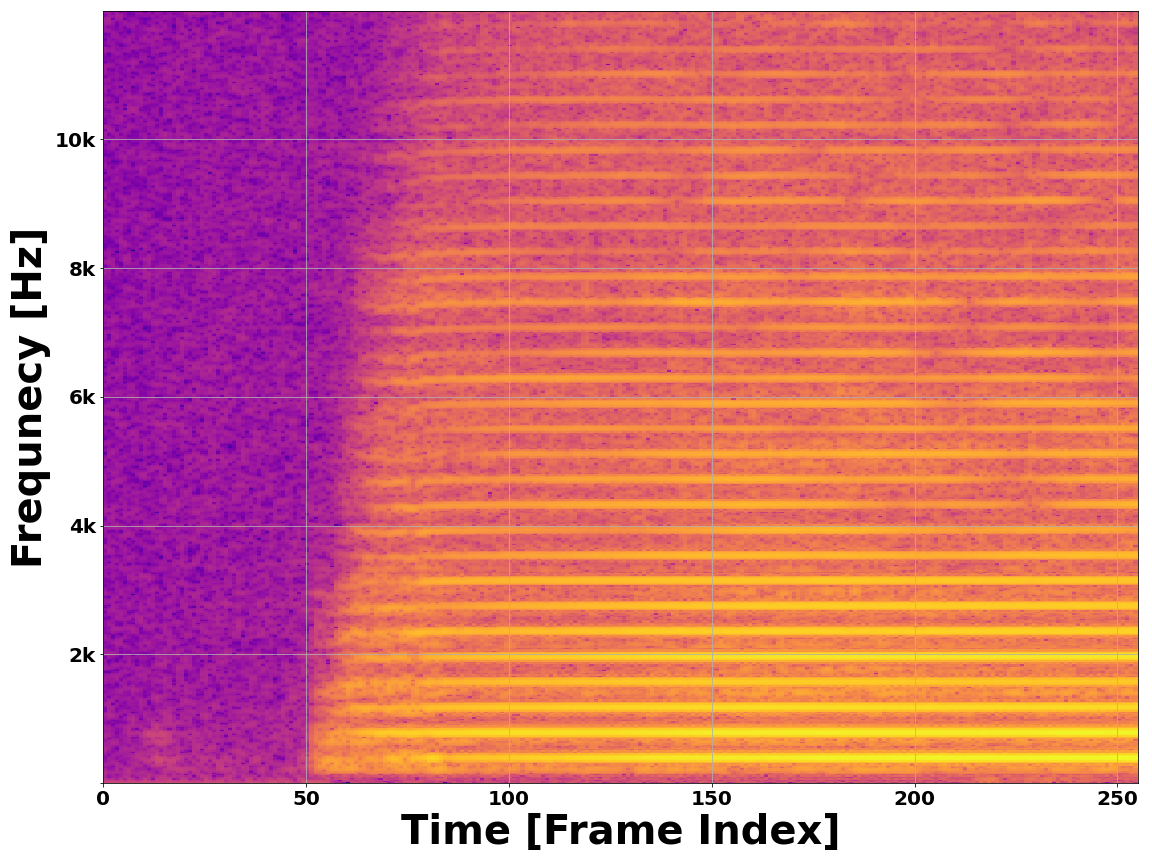
\includegraphics[scale=0.2]{../FiguresSpectrogram/Viola-G4}
	\caption{Viola playing $G4$}
	\end{subfigure}
\caption{Spectrograms from chordophone waveforms}	
\label{fig-PropertiesChordophones}
\end{figure}

\paragraph*{}The wave equation is a \textit{linear} partial differential equation which allows for a linear combination of solutions to form a sound wave. In the case of the taught finite string that is fixed at both ends, such a guitar, viola or cello, the a solution tends to take the form of a sine or cosine function \cite{Hunter, Taylor, White}. Notice the terms arise by the many a parallel yellow and orange lines in each spectrogram in Fig. (\ref{fig-PropertiesChordophone}). The verical position of any line is given by the linear frequency of the sinusoid, and the brightness is proportional to the coefficient of the combination. The boundary conditions, and most forms of standard initial conditions allow for the each sinusoidal to fit exactly an integer or half-integer number wavelengths into the region $0 \leq x \leq L$ \cite{Haberman,Hunter}. Players of chordophones change pitch by shortening the length of the vibrating string or applying additional tension to the string. This changes the length of portion of the string that vibrates, and causes the production of a new pitch.

\paragraph*{}Each chordophone instrument does produce a slightly different frequency spectrum, hence each provides a slightly different timbre to the listener, so differentiating between them is possible. Because of this, we find that the spectrogram representation of the waveform is so critical to classification success because the convolution layers allow for the detection of small variations in the frequency-time domain where humans would otherwise be unable to \cite{Loy,Virtanen}. However, the size of the instrument limits the length of the string that vibrates which leads to limitations in the range of the overtones the instruments will produce. For example, a cello playing a low $C1$ will have overtones extending up into the $12$ kHz range, but the energy will be very low there, thus have a very low frequency center of mass. Compare this with a violin playing a $C6$, will have overtones into the $20$ kHz range, and will produce a very high frequency center of mass. While the ranges of the musical instruments overlap a great deal, the energy distribution in frequency space can be treated as a 1D mass distribution, and the frequency center of masses of instruments with similar timbres can still differ greatly \cite{Serizel}.

\paragraph*{}Notice as well in the spectrograms of Fig. (\ref{fig-PropertiesChordophones}), how the transient response (the time domain) of chordophones differs wildly from idiophones and membranophones. In the case of bowed instruments, the attack of the stringed instrument is much longer, with a much more gradual sustain decay, and release. Where an idiophone or plucked string has all of the time-domain energy up front, the bowed string waveform continues to build energy as the instrument is bowed, and only loses energy once the bowing stops, and the string is left to vibrate by itself \cite{Hunter}. This causes a bowed stringed instruments to present a very different amplitude envelope compared to the other categories of instruments, and a much more centrally located temporal center of mass.

% ================================================================

\subsection{Aerophones}
\label{subsec-Aerophones}

\paragraph*{}An aerophone is a musical instrument that produces sounds through the vibration of an air molecules in a column-like structure. This is the largest category of instruments that we have, and is commonly broken down into smaller subcategories such as \textit{woodwind} and \textit{brass} instruments. From our data set - alto flutes, alto saxophones, bass clarinets, bass flutes, bassoons, $B\flat$ clarinets, contrabassoons, $E\flat$ clarinets, English horns, flutes, oboes, tenor saxophones, and soprano saxophones are all examples of woodwind aerophones. Additionally, bass trombones, french horns, tenor trombones, trombones, $B\flat$ trumpets, and tubas are all examples of brass aerophones \cite{Hornbostel,Olson,White}.

\paragraph*{}Aerophones all produce sound by exciting molecules of air within a column that vibrates in different patterns called \textit{modes} \cite{White}. the wavelength and energy of each mode is  determined by the structure of the instruments, and the actions of the player. Most aerophones such a flutes, clarinets, and saxophones are more much more reminiscent of air columns that are closed at one end and open at the other. This is marked by the presence of a mouth piece at one end where a played blows air from their lungs to add energy, and a bell at the other end to serve as an amplification structure \cite{Olson}. For a column of length $L$, that is open at one end, the fundamental frequency of the vibration is given by \cite{Olson}:
\begin{equation}
\label{eqn-OpenClosedCol}
f_0 = \frac{v}{4L} = \frac{v}{\lambda}
\end{equation}
where $v$ is the velocity of sound in the medium, and $\lambda$ is the wavelength of the sound wave. Eq. (\cite{eqn-OpenClosedCol}) gives the lowest pitch that such an instrument with a length $L$ can play. Lower woodwinds such as bass clarinets, have a much longer vibrating air column that that of the much shorter piccolo, thus can produce considerably lower notes.

\paragraph*{}To change the pitch, the performer of an aerophone must change the length of the vibrating air column by pressing keys with their fingers. This causes a different number of wavelengths to fit within the column, and thus change the note being played. Shortening the column (reducing $L$) also causes a reduction in the wavelength, and an increase in frequnecy and vice-versa. In Fig. (\ref{fig-PropertiesAerophonesWind}) we show the spectrogram waveforms for a few different woodwind instruments.

\begin{figure}[H]
	\begin{subfigure}{0.45\textwidth}
	\centering
	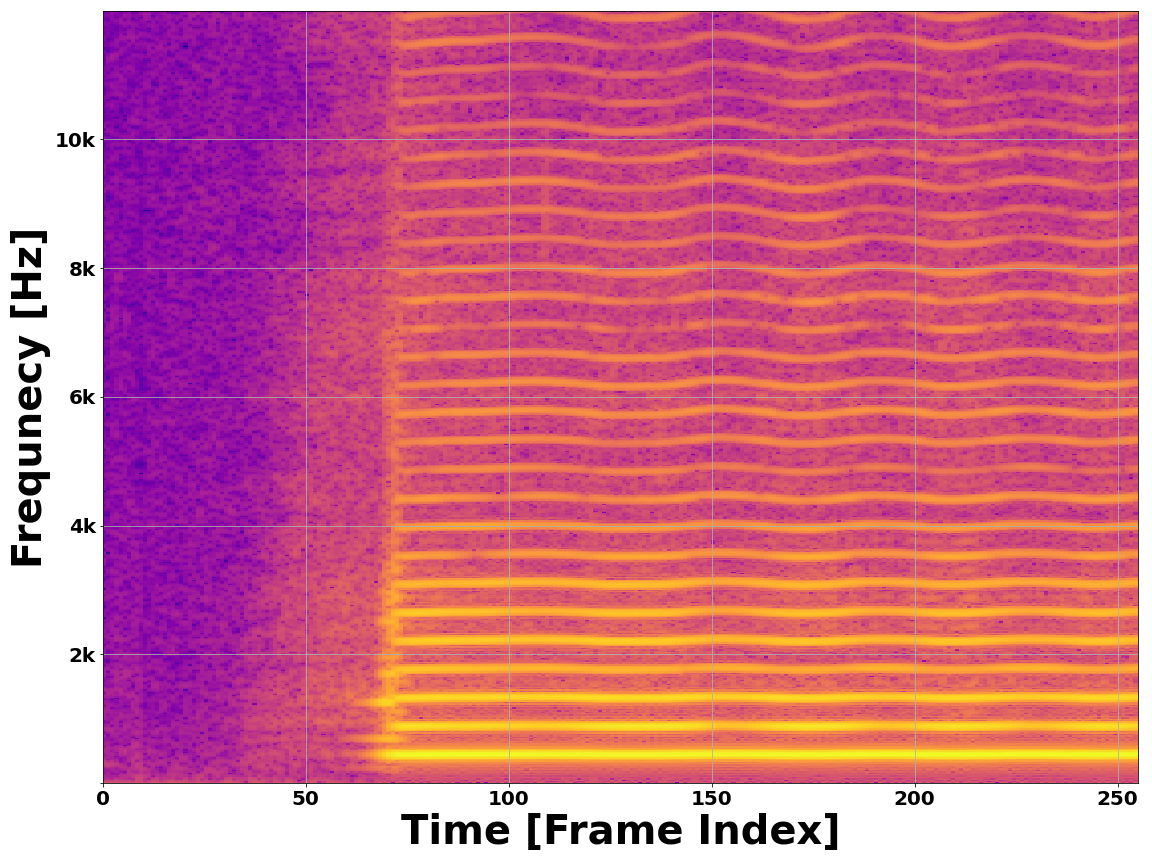
\includegraphics[scale=0.2]{../FiguresSpectrogram/AltoSax-A4}
	\caption{Alto Saxophone playing $A4$}
	\end{subfigure}
	\hfill
	\begin{subfigure}{0.45\textwidth}
	\centering
	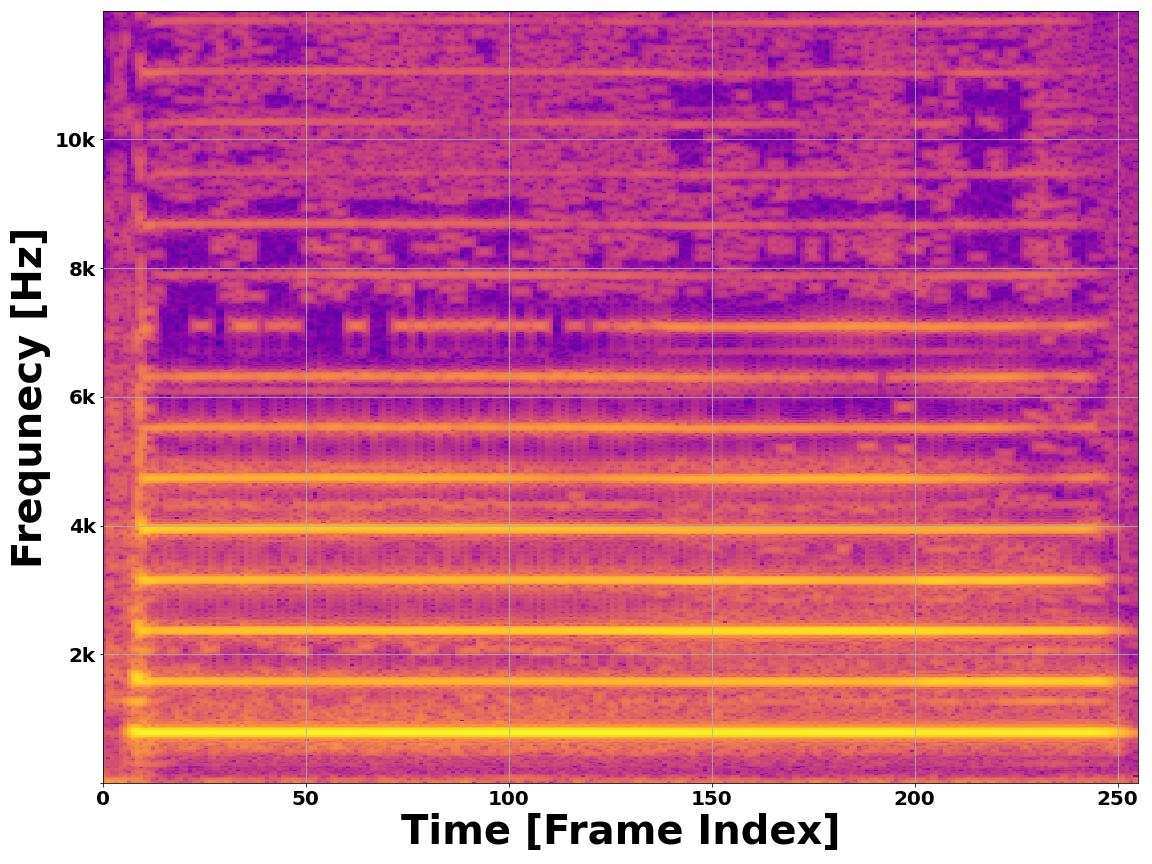
\includegraphics[scale=0.2]{../FiguresSpectrogram/Clarinet-Gs5}
	\caption{$B\flat$ Clarinet playing $G\sharp 5$}
	\end{subfigure}
	
	\begin{subfigure}{0.45\textwidth}
	\centering
	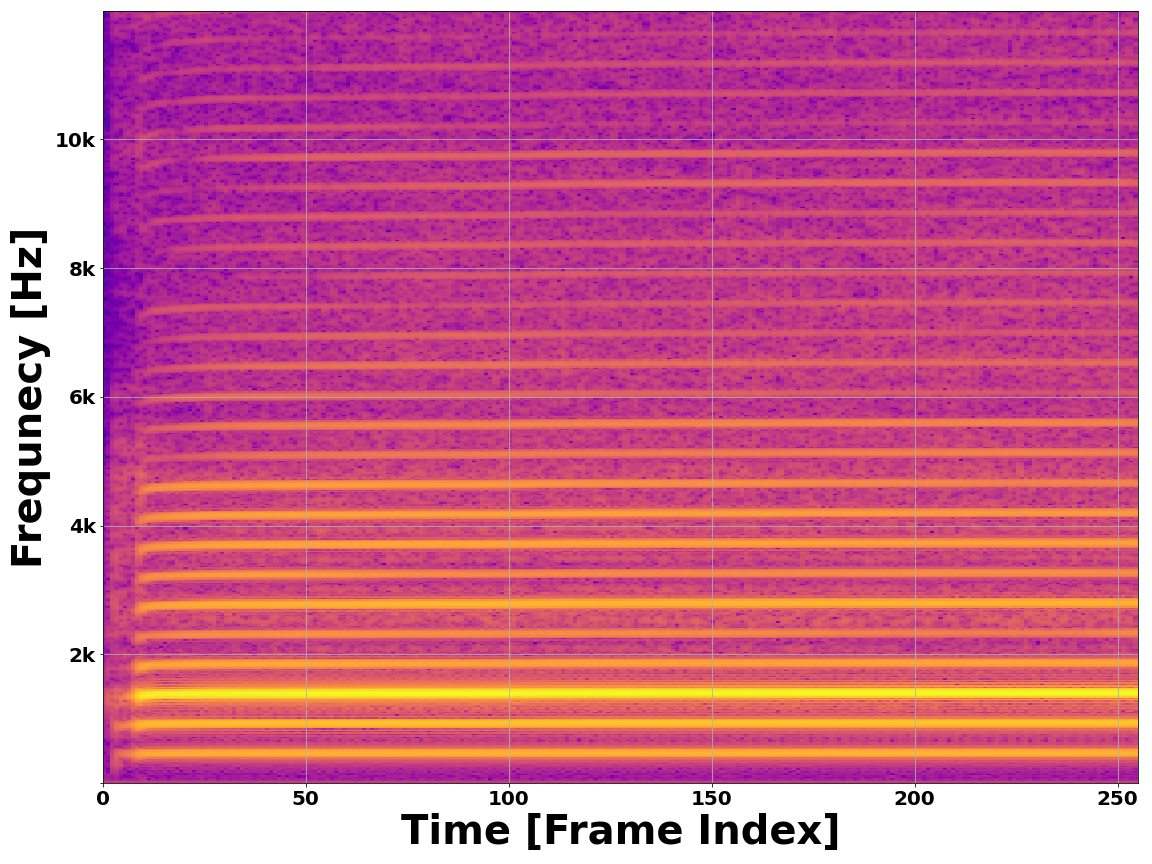
\includegraphics[scale=0.2]{../FiguresSpectrogram/Oboe-Bb4}
	\caption{Oboe playing $B\flat 4$}
	\end{subfigure}
	\hfill
	\begin{subfigure}{0.45\textwidth}
	\centering
	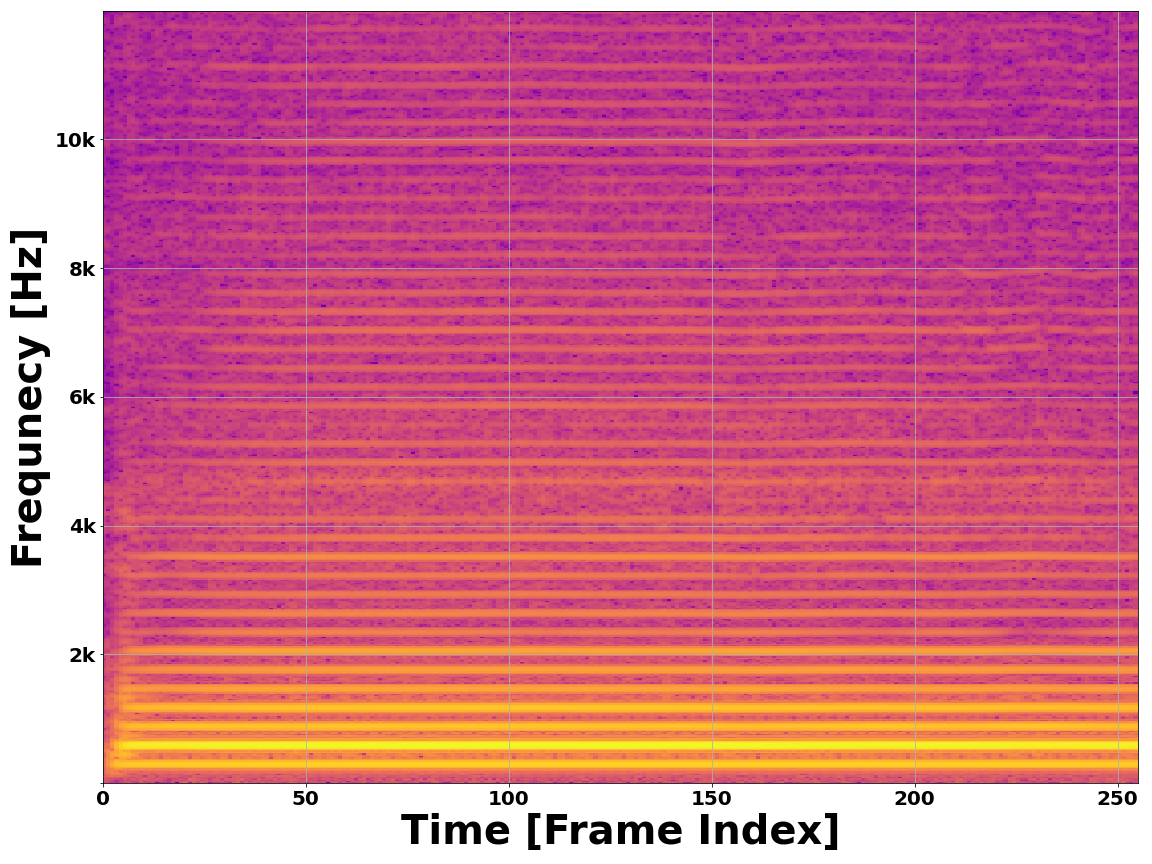
\includegraphics[scale=0.2]{../FiguresSpectrogram/Bassoon-D4}
	\caption{Bassoon playing $D4$}
	\end{subfigure}
\caption{Spectrograms from woodwind aerophone waveforms}	
\label{fig-PropertiesAerophonesWind}
\end{figure}

\paragraph*{}In addition to the woodwind instruments described above , we also consider the properties of brass aerophones. As the name implies, brass instruments are usually made of interconnected hollow tubes of brass as opposed to linear columns of mostly wood. Brass aerophones are also modeled as open-closed columns that vibrate and are also shortened and lengthened by pressing keys. Brass instruments are generally much longer than woodwinds, and produce sounds at a generally greater volume \cite{Olson}. Despite these differences, brass instruments do generally display a great deal of similarities with wood winds, as shown in Fig. (\ref{fig-PropertiesAerophonesBrass})

\begin{figure}[H]
	\begin{subfigure}{0.45\textwidth}
	\centering
	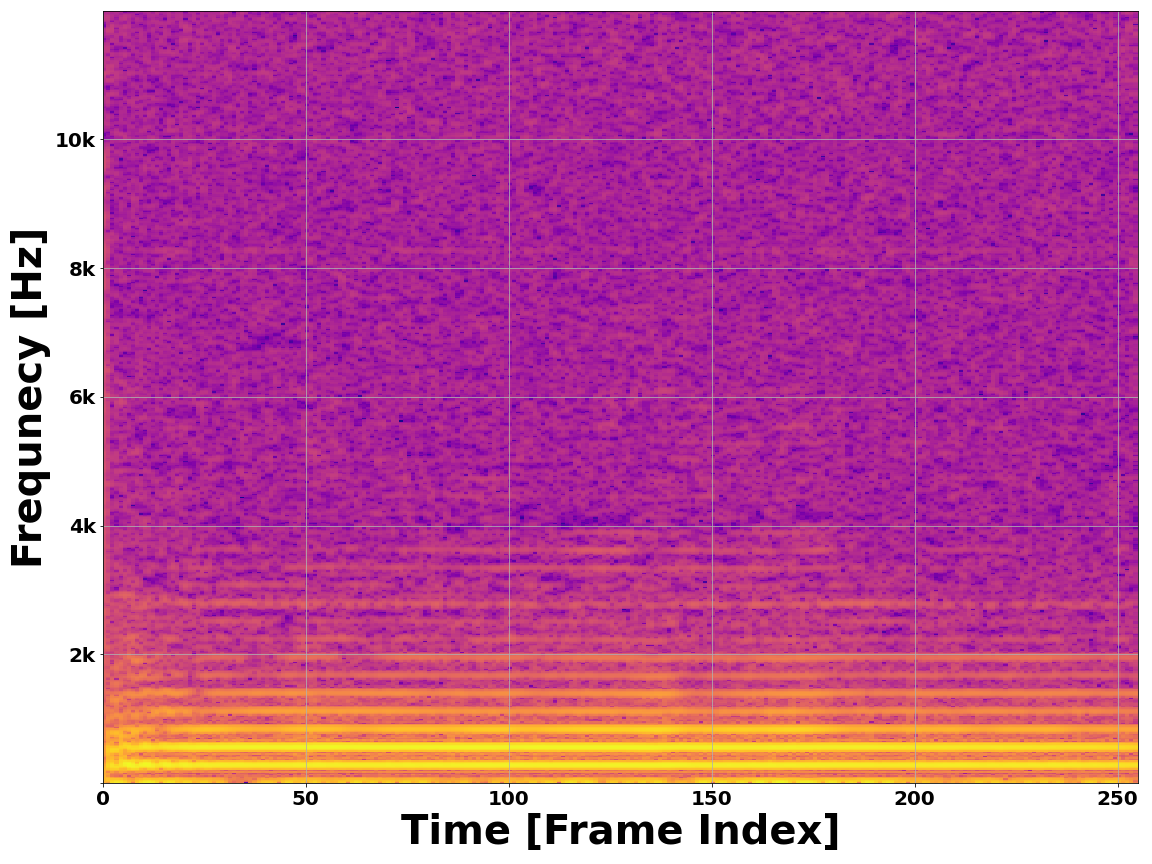
\includegraphics[scale=0.2]{../FiguresSpectrogram/FRENCHHORN-Cs4}
	\caption{French horn playing $c\sharp 4$}
	\end{subfigure}
	\hfill
	\begin{subfigure}{0.45\textwidth}
	\centering
	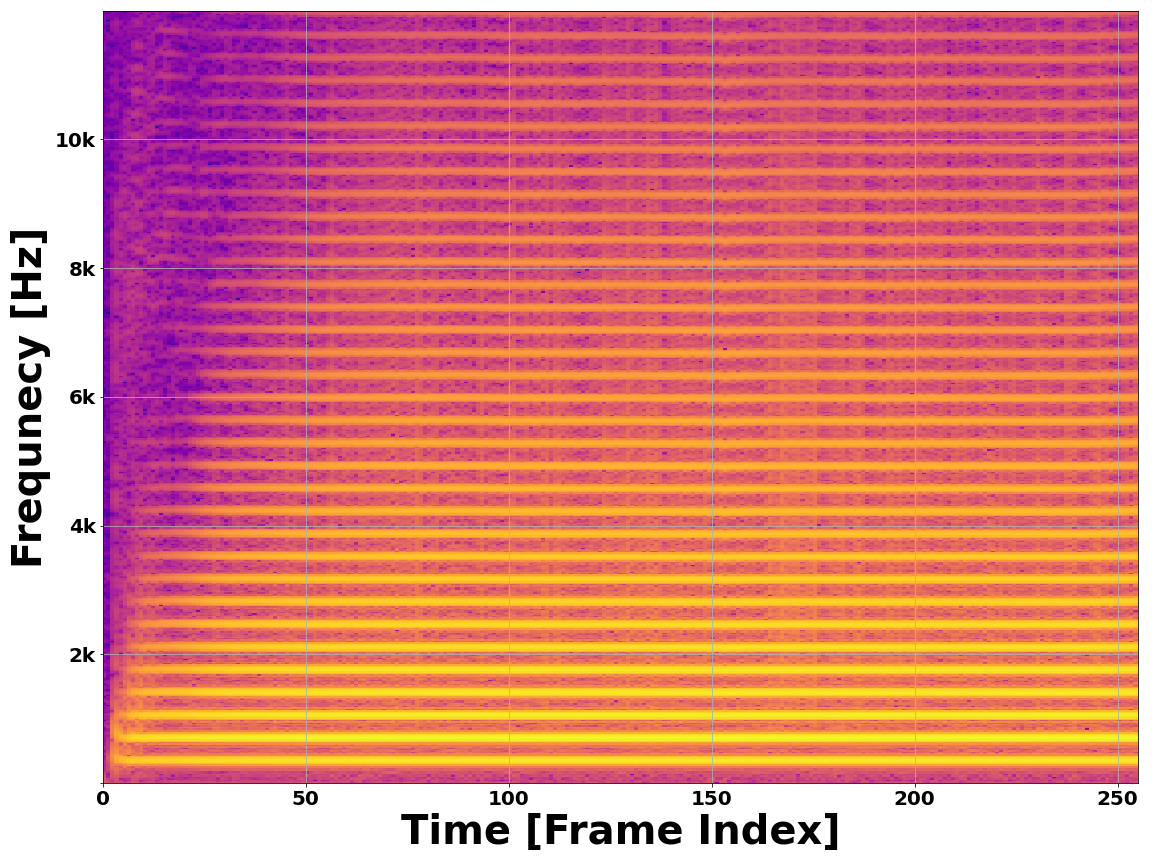
\includegraphics[scale=0.2]{../FiguresSpectrogram/TenorTrombone-F4}
	\caption{Tenor Trombone playing $F4$}
	\end{subfigure}
	
	\begin{subfigure}{0.45\textwidth}
	\centering
	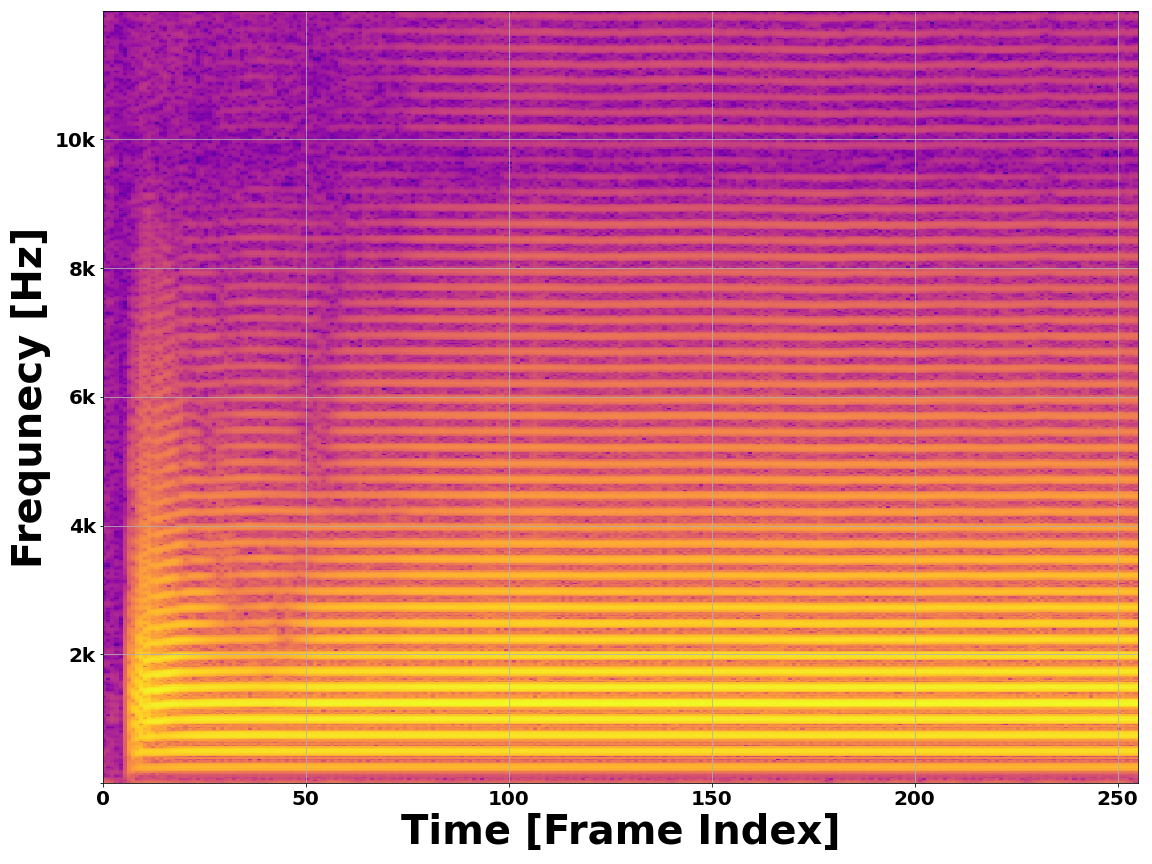
\includegraphics[scale=0.2]{../FiguresSpectrogram/Trumpet-B3}
	\caption{$B\flat$ Trumpet playing $B3$}
	\end{subfigure}
	\hfill
	\begin{subfigure}{0.45\textwidth}
	\centering
	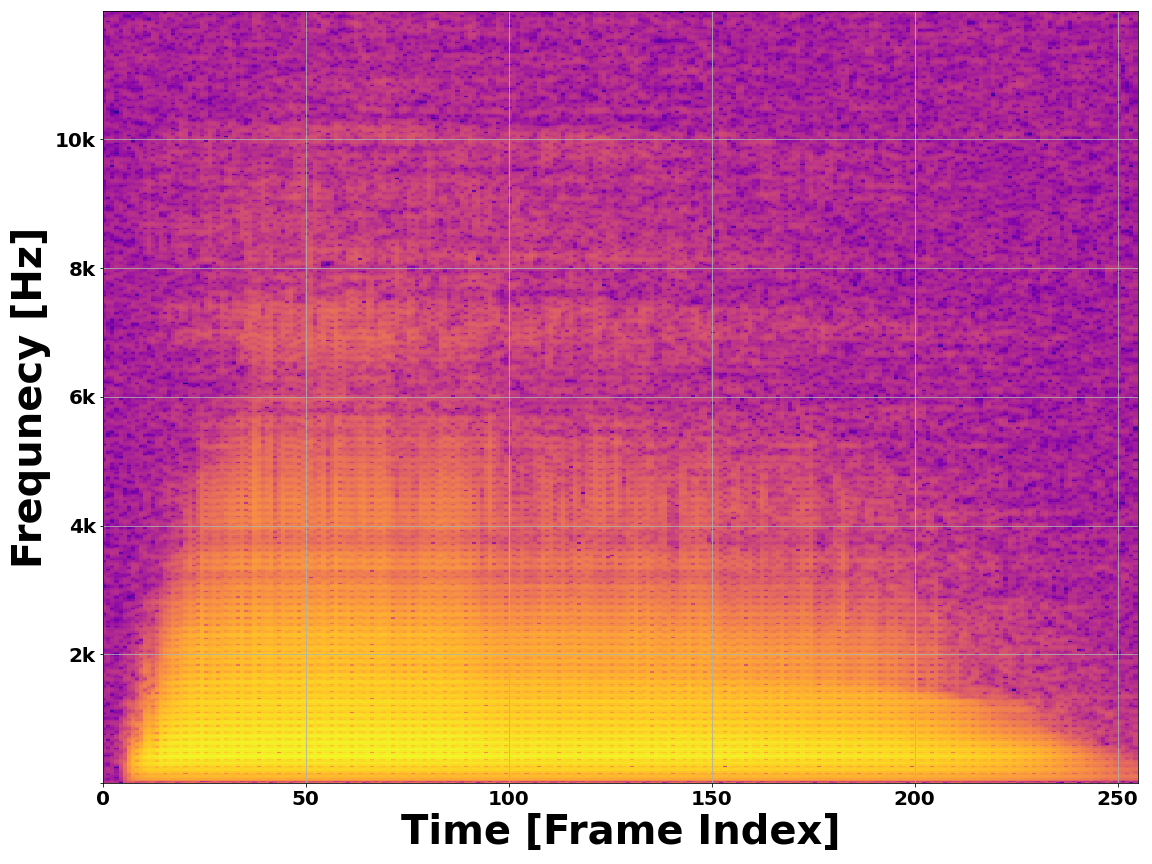
\includegraphics[scale=0.2]{../FiguresSpectrogram/Tuba-A2}
	\caption{Tuba playing $A2$}
	\end{subfigure}
\caption{Spectrograms from brass aerophone waveforms}	
\label{fig-PropertiesAerophonesBrass}
\end{figure}

\paragraph*{}Just like with idiophones and chordophones, the amplitude envelop of a brass instrument is very characteristic. Aerophones require a user to vibrate air with their lungs which gradually adds energy to the waveform. This transfer of energy can take comparably long time, giving aerophones particularity long attack times when compared to idiophones or membranophones. The note is sustained as long as a player is vibrating the air, allowing for any length of decay and sustain, but the energy does out very suddenly when the player stops, giving a characteristically short release time \cite{White}. 

% ================================================================

\subsection{Other Generated Sounds}
\label{subsec-Generated}

\paragraph*{}We group sounds produced from non-physical musical instruments in this final category because they are not considered in the original Hornbostel-Sachs system. From our data set, this category includes the four simplest waveforms begin, sine waves, sawtooth waves, square waves, and triangle waves, as well as white colored noise \cite{White}. These sounds have been produced synthetically through a MATLAB program specifically for this project. Because of their synthetic nature, they do not display many of the physical or mechanical properties of the previous sections.

\paragraph*{}Each of the five synthetically generated waveform types were produce to have a constant envelope with all time. This means that each waveform has no characteristic amplitude shape and the spectrogram shows no time-evolution of energy as expected. Each of the the signals can be composed of a linear combinations of oscillating sinusoidal at various different frequencies and energies. For example, a sine wave consists only of a single oscillating term, while a square wave consists of repeated odd harmonics. White noise consists of a roughly uniform distribution of energy, thus shows no energy evolution in time or frequency space. These behaviors can be observed in Fig. (\ref{fig-PropertiesSynths}).

\begin{figure}[H]
	\begin{subfigure}{0.45\textwidth}
	\centering
	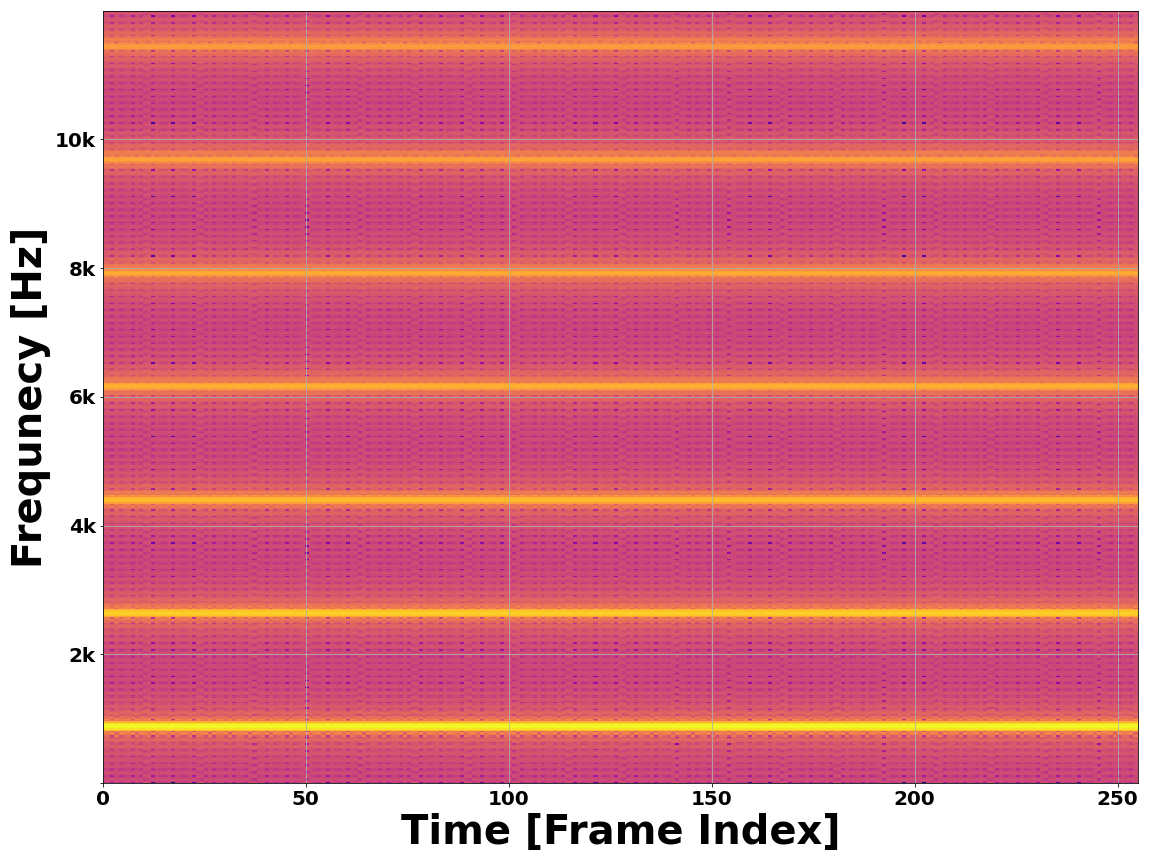
\includegraphics[scale=0.2]{../FiguresSpectrogram/SquareWave-880Hz}
	\caption{Square Wave at $880$ Hz}
	\end{subfigure}
	\begin{subfigure}{0.45\textwidth}
	\centering
	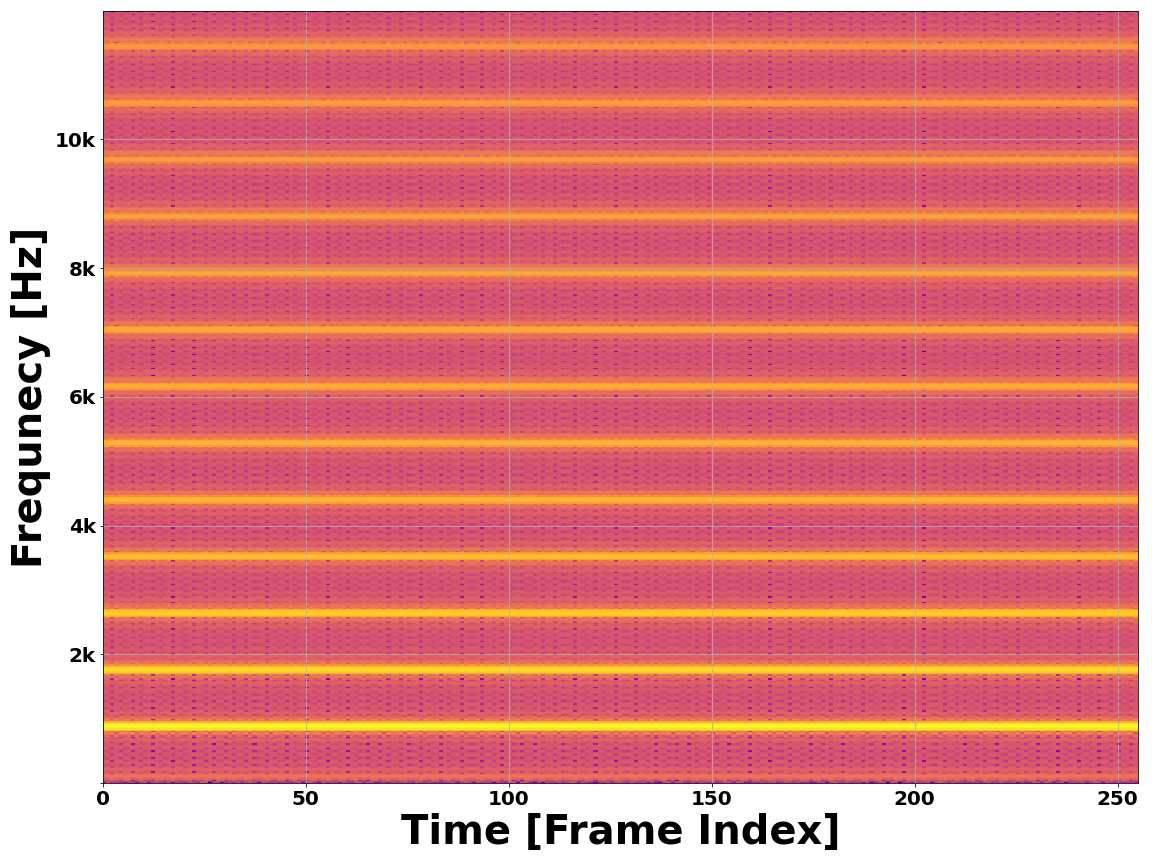
\includegraphics[scale=0.2]{../FiguresSpectrogram/SawtoothWave-880Hz}
	\caption{Sawtooth Wave at $880$ Hz}
	\end{subfigure}
	
	\begin{subfigure}{0.45\textwidth}
	\centering
	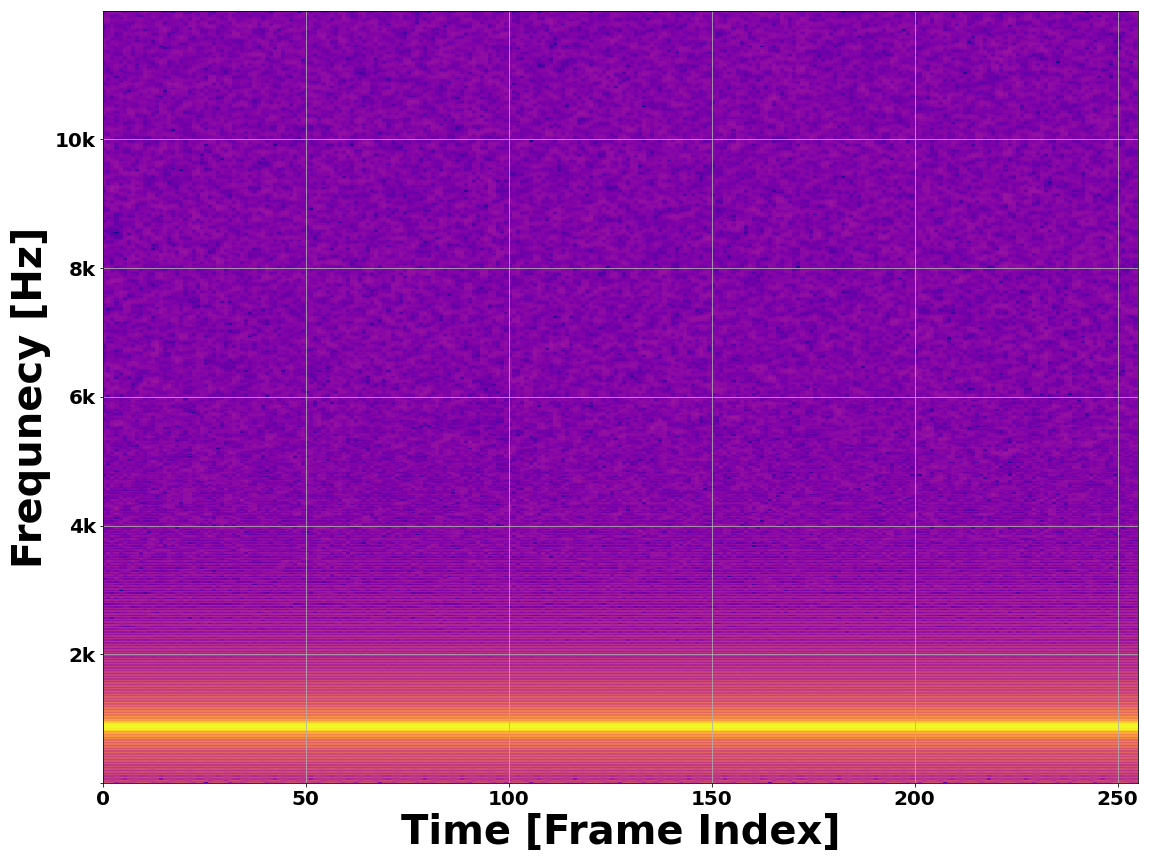
\includegraphics[scale=0.2]{../FiguresSpectrogram/SineWave-880Hz}
	\caption{Sine Wave at $880$ Hz}
	\end{subfigure}
	\begin{subfigure}{0.45\textwidth}
	\centering
	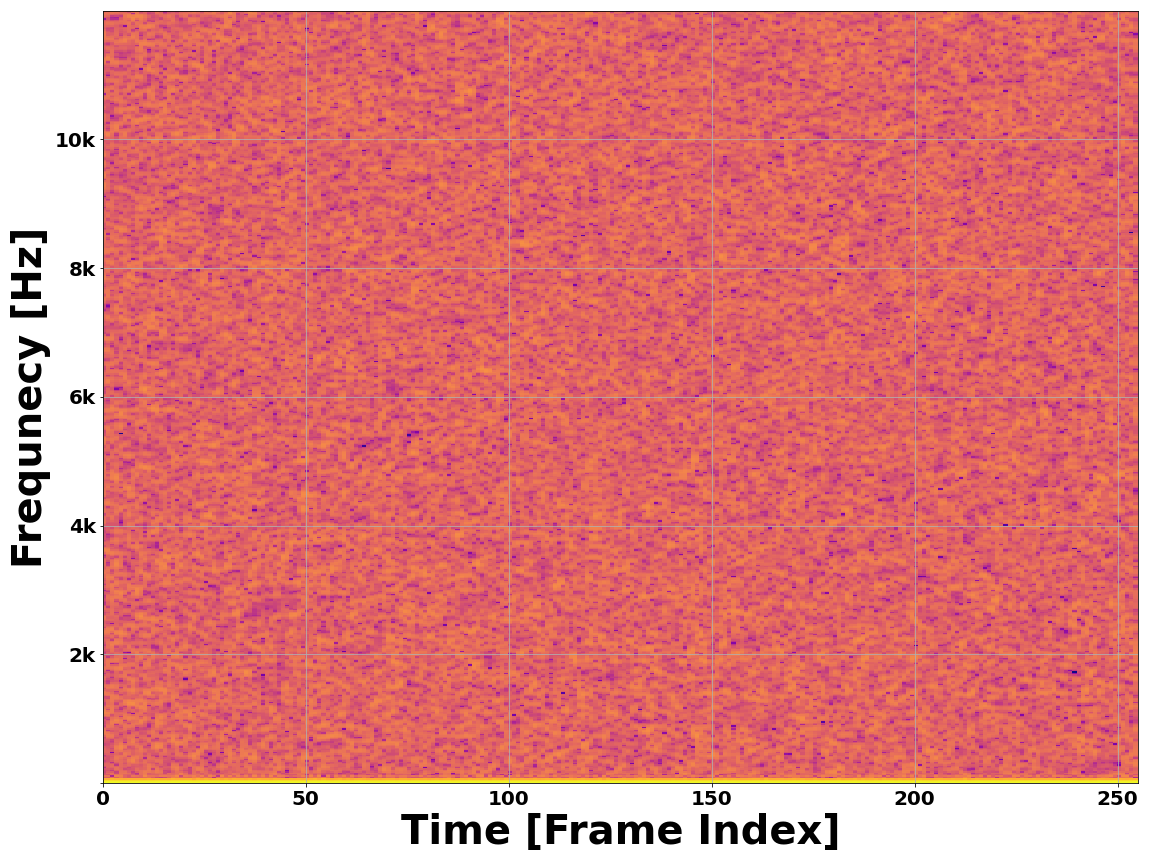
\includegraphics[scale=0.2]{../FiguresSpectrogram/WhiteNoise-190}
	\caption{White Noise}
	\end{subfigure}
\caption{Spectrograms from synethetically generated waveforms}	
\label{fig-PropertiesSynths}
\end{figure}

These waveforms were included to our data set to serve as a control to understand how the chosen features respond to simple waveforms. Additionally, the elementary composition of each waveform allows for it to potentially resemble a wide variety of instrument frequency spectra \cite{White}.


% ================================================================
% ================================================================

\newpage
\section{Feature Selections}
\label{sec-Features}

\paragraph*{}Classification tasks require a set of inputs called \textit{predictors} or \textit{features} \cite{James,Loy,Serizel}. A feature is a quantitative, low-dimensional representation of a sample that conveys its important characteristics. For example, in classifying types of animals, a feature could be the mass, volume or number of teeth on the animal. Typically, we produce a set of $p$ features for each sample and assemble them into a $p$-dimensional vector called a \textit{feature vector} which acts as a list of descriptive qualities of the sample \cite{Geron,James}. This list is presented to the neural network and used to 
Audio machine learning researchers M. Kashif Saeed Khan and Wasfi G. Al-Khatib describe the vitality of feature selection \cite{Khan}:
\begin{quote}
The data reduction stage which is also called feature extraction, consists of discovering a few important facts about each class. The choice of features is critical as it greatly affects the accuracy of audio classification. 
\end{quote}
An adequate selection of features is vital to the process of training and evaluation of the classifier model \cite{Mierswa,Serizel,Liu}. Consider the task of identifying fish from sharks using only the presence of gills. Since both sharks and fish have gills, the features are correct representations, but not useful for discerning them. A more appropriate choice would be compare the number of gills that fish or sharks have, which would provide a correct representation and allows for differentiation.

\paragraph*{}In the biological process of categorizing sound sources, the time-domain waveform is usually enough to match the sound to a source \cite{Olson}. However, a computer representation of a waveform is an array-like structure of values sampled discretely in time and volume \cite{Virtanen,Liu}. Presenting the raw time-series waveform to a model directly has experimentally shown to be unstable in for classification tasks so we must develop a set of features that can describe important properties of the waveform in a far more efficient manner \cite{Goodfellow,James,Serizel}. To ensure the construction of a suitable model, we derive features based from three representations of the audio file: (i) a spectrogram matrix, (ii) the time-space, and (iii) the frequency-space. It is important to note that although this algorithm will map audio files to source instruments, it will never actually be presented with a waveform directly, and instead will rely solely on the features to make predictions.

% ================================================================

\subsection{Feature Space}

\paragraph*{}From each audio file sample, we calculate the values for the same predictors. The predictors are arranged into two separated structures, each called a \textit{design matrix}, described in section (\ref{subsubsec-DesignMatrix}) \cite{Goodfellow,Geron}. For a model with $p$ predictors, feature space is a $p$-dimensional vector space where each basis vector represents a predictor \cite{Goodfellow,James}. Each sample can be described by a $p$-dimensional vector, given by each row of the design matrix $X_2$. For samples $x^{(a)}$ and $x^{(b)}$ that belong to the same class, we expect the vector to be similar, $x^{(a)} \approx x^{(b)}$ in some way. This indicates that the two samples lie "close together" in space. Similarly, for samples $x^{(c)}$ and $x^{(d)}$ that belong to different classes, we expect the vectors to be very different, indicating that the two sample lie "far apart" in space. Note that this is an idealization, and not always the defining case for the decision function behavior.

\paragraph*{}We can expand this idea by considering by how features should behave within each class, and between each class. Tuomas Virtanen, machine learning and audio engineer writes in his book, "Computational Analysis of Sound Scene and Events" about specifically how features should be selected \cite{Virtanen}:
\begin{quote}
For recognition algorithms, the necessary property of the acoustic features is low variability among features extracted from examples assigned to the same class, and at the same time high variability allowing distinction between features extracted from examples assigned to different classes.
\end{quote}
This is to say, features should \textit{ideally} form non-overlapping groups or bubbles that allows classifiers to effectively differentiate categories. Given the complexity of real-world problems, this is an often unobtainable \cite{Goodfellow,James}. Under the right circumstances, classifiers can still produce parameters that allow for reasonable performance \cite{Geron,Loy}. In practice, a neural network does not rely on comparing the norms of different samples in feature space, but rather uses something called a \textit{decision boundary}.

\subsubsection{Decision Boundaries}
\label{subsubsec-Decision}

\paragraph*{}A trained classifier makes a prediction in the form of a statistical likelihood of a sample belonging to a particular class \cite{Goodfellow,James}. A $k$- categories classifier contains $k$ output neurons, each one representing a different class. When a set of features is presented to the classifier, the value contained within each neuron is the "confidence" on the interval $[0,1]$ that a sample belongs to that class. For example, if neuron $q$ has an activation value of $0.25$, we say that there is a $25\%$ chance that the sample belongs to class $q$. Most commonly, we take the neuron with the highest activation value to be the chosen class, even if the next highest activation is a close second \cite{Loy}. Thus the formal prediction function is the index of the maximum value in the output vector.

\paragraph*{}This concept stems from the idea that when a trained neural network classifier makes a prediction, it is basing class probabilities on a set of generated \textit{decision boundaries} \cite{Geron,James}. To explore decision boundaries, consider a simplified toy data set with a 2D feature space for a classifier that must only discern between \textit{Class A} and \textit{Class B}. We can visualize each sample in this 2D space, and color-code each sample according according to it's class label as in Fig. (\ref{fig-LinSep1}).

\begin{figure}[H]
\begin{center}
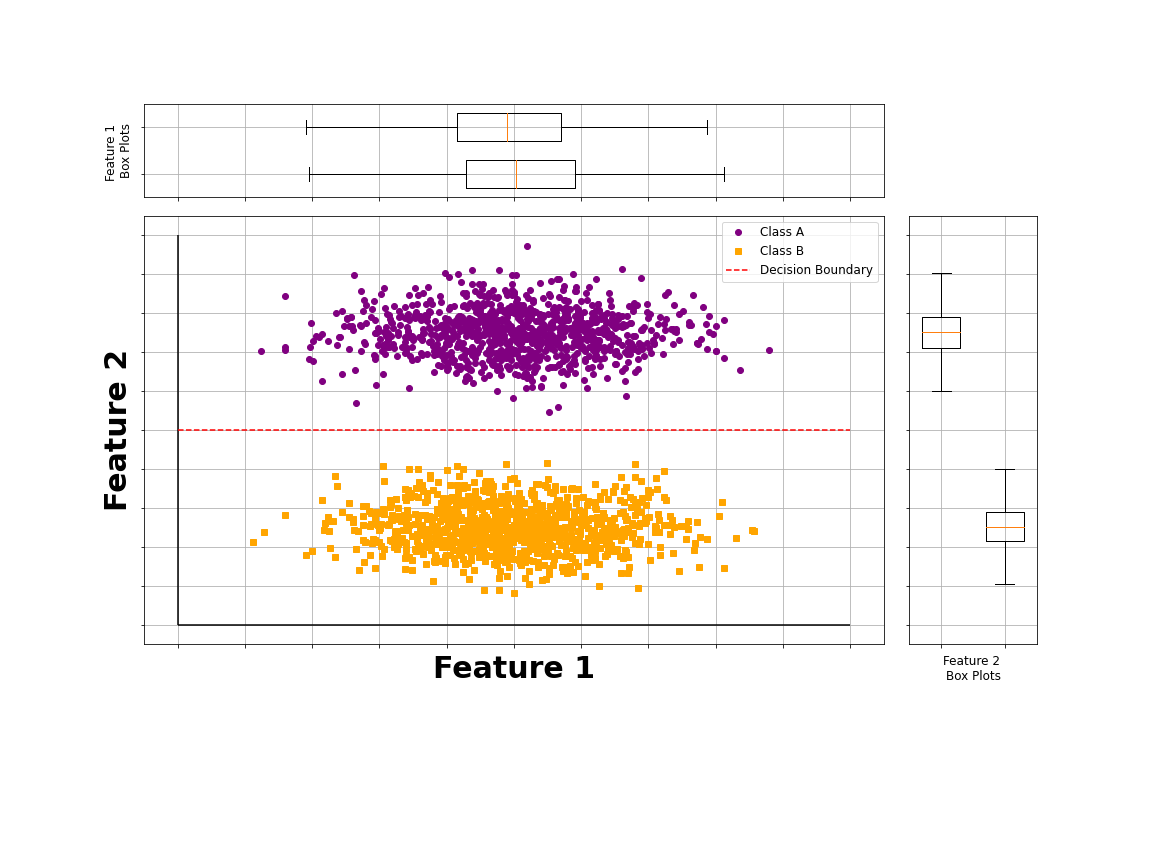
\includegraphics[scale=0.35]{../MakeFigures/LinearSeparable1}
\end{center}
\caption{Feature Space with Linear separability between two classes}
\label{fig-LinSep1}
\end{figure} 

\paragraph*{}In the case of these chosen, features, we can see a clear, well-defined separation between samples in each class. In practice, this is rarely the case, but shows graphically an example where a linear decision boundary arises \cite{James}. Notice how we can also use "box-and-whisker plots" to neatly summarize how each feature (each component) behaves by dividing the samples for each class based into quartiles. Notice how on the right of Fig.(\ref{fig-LinSep1}) the box plots for feature 2 show no overlap, but the box plots for feature 1, at the top show very similar behavior between classes. Despite this, a classifier can produce a clean boundary to separate the two classes. Note that this may not be the exact boundary used by a model, but it represents an ideal case.

\paragraph*{}We can also explore an example where both features have mutual overlap between classes, but we can still form a reasonable decision boundary in the space. Consider Fig. (\ref{fig-LinSep2}) and Fig. (\ref{fig-LinNonSep}). In both cases, we see the box plot for each feature overlap considerably, and we also see sample that appear to "cross" the decision boundary. This crossing the boundary is why it is so useful that we choose an activation function that encode the output of the neural network as a probability of being in either class as opposed to a hard prediction \cite{Loy,Geron}.

\begin{figure}[H]
\begin{center}
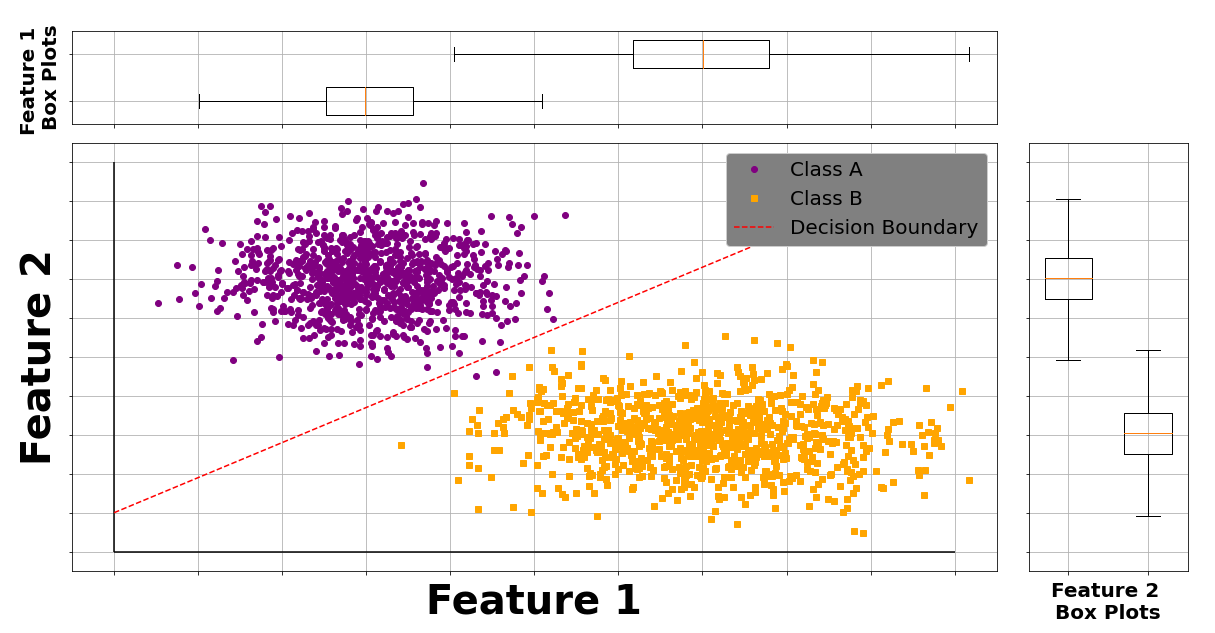
\includegraphics[scale=0.35]{../MakeFigures/LinearSeparable2}
\end{center}
\caption{Feature Space with near linear separability between two classes}
\label{fig-LinSep2}
\end{figure}

\begin{figure}[H]
\begin{center}
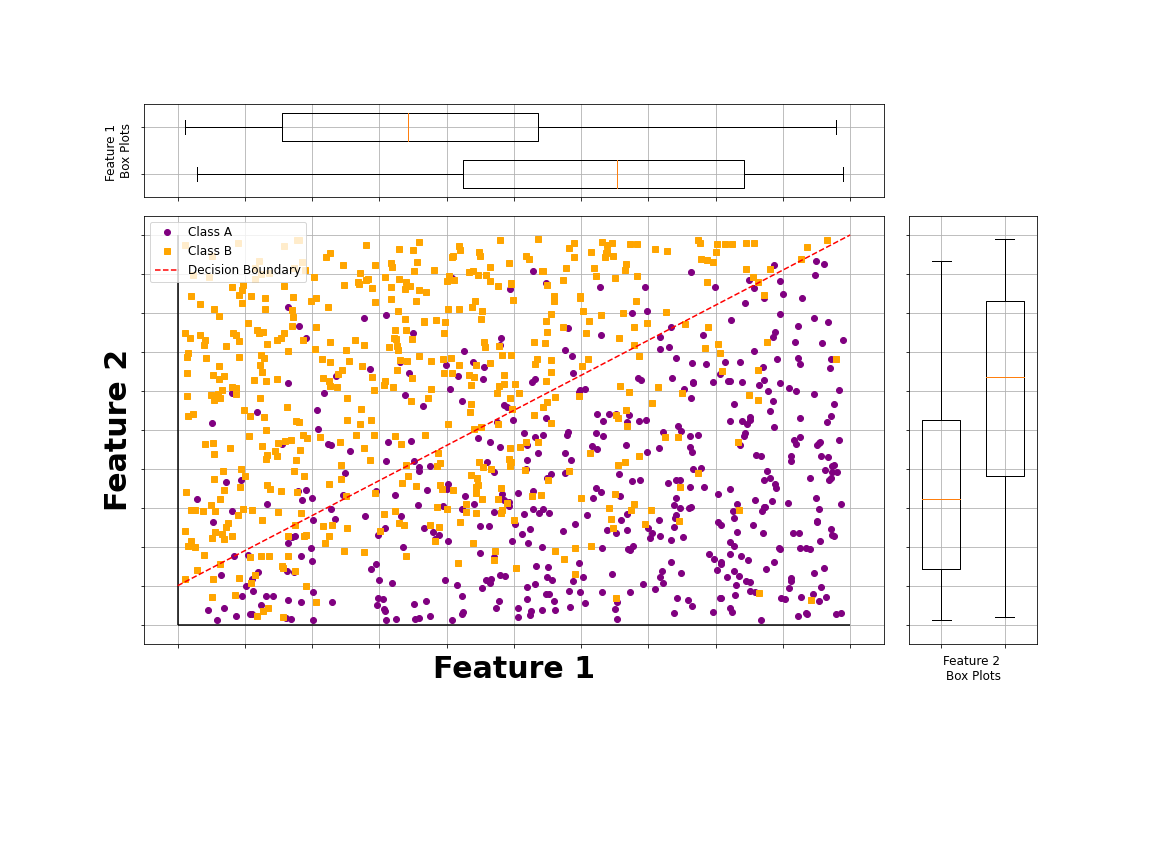
\includegraphics[scale=0.35]{../MakeFigures/LinearNonSeparable}
\end{center}
\caption{Feature Space with near linear non-separability between two classes}
\label{fig-LinNonSep}
\end{figure}

\paragraph*{}Samples that appear very near to decision boundary will likely have almost equal probability of occurring in either class, and samples that appear very far from the decision boundary will likely have very much larger probability of occurring in one class or the other \cite{Bishop,James}. 

\paragraph*{}Note that these are over-idealized cases, constrained to two classes in two dimensions. The classifier implemented in this project uses $24$ classes in a single branch and outlines a probabilty estimate over $37$ classes. Given the related nature of many of the categories, (i.e. belonging to similar Hornbostel-Sachs groups), such well-defined decision boundaries are unlikely to be produced. Note also that the examples provided showed only \textit{linear} boundaries, where the inclusion of non-linear activation functions will create far more complex systems in a far higher-dimensional space \cite{Goodfellow}.

\paragraph*{}From these examples, we conclude the mathematical nature of features allow each sample to be characterized by a vector in $p$-dimensional feature-space \cite{Goodfellow,James}. We expect feature of the same class to exhibit similar characteristics, and features of differing classes to exhibit different characteristics. This enables a trained classifier to develop multiple decision boundaries in the higher-dimensional space \cite{James,Bishop}.

% ================================

\subsubsection{The Design Matrix}
\label{subsubsec-DesignMatrix}

\paragraph*{}Each audio sample is represented by an $N' \times k$ spectrogram matrix explored in section (\ref{subsec-Spectrogram}), a $1 \times p$ feature vector, and a  one-hot-encoded target label, $y$. In order to efficiently present the information to the model for training or predicting, we extract a batch of $b$ samples and produce the two arrays form each. Since the spectrogram and feature vector represent different \textit{modalities}, we construct two separate \textit{design matrices}, $X_1$ and $X_2$ \cite{Geron,Li,Ngiam}. Each has shape given by:
\begin{equation}
\label{eqn-X1Shape}
X_1 \in \mathbb{R}^{(b \times N' \times k)}
\end{equation}
\begin{equation}
\label{eqn-X2Shape}
X_2 \in \mathbb{R}^{(b \times p)}
\end{equation}
Where $N' \times k$ gives the shape of the spectrogram matrix $S$ from a single sample, described in section (\ref{subsec-Spectrogram}). Similarly, $p$ is the number of predictors extracted from each sample, outlined in section (\ref{subsec-TimeFeatures}) and section(\ref{subsec-FreqFeatures}). The first axis, with size $b$ indicates that there are $b$ audio file samples stored in that design matrix. Organizing the samples in this fashion allows for easy machine and human interpretation of each axis and index.

\paragraph*{}A design matrix is typically accompanied by a \textit{target matrix} $Y$, which indicates the class that the particular sample belongs to. For a classifier with $\kappa$ classes, each sample labeled by a one-hot-encoded vector for shape $1 \times \kappa$ \cite{Tensorflow,Loy}. Thus, for the design matrices $X_1$ and $X_2$, we have a corresponding target matrix given by:
\begin{equation}
\label{eqn-YShape}
Y \in \mathbb{R}^{(b \times \kappa)}
\end{equation}

% ================================

\subsubsection{Audio Preprocessing}
\label{subsubsec-Preprocessing}

\paragraph*{}Preprocessing a data set is a necessary step to execute prior to feature extraction \cite{Geron2,James,Serizel}. In the case of audio files, preprocessing usually consists of ensuring that the data set contains the following steps and requirements:
\begin{enumerate}
\item A suitably sized number of files of reasonable audio quality with normalized amplitudes
\item Audio encoded in a standard, and consistent format
\item A consistent sample rate and bit depth between audio files
\item A consistent number of channels
\end{enumerate}
Note that different projects may require a different set of requirement from preprocessing \cite{Virtanen}. For this project, we have chosen to use the following parameters:
\begin{enumerate}
\item Roughly $18,000$ audio files Professionally or semi-professionally recorded in a studio \cite{Philharmonia,UnivIowa} All ampltiudes have been normalized to $\pm 1$ unit.
\item All audio has be converted into \textit{.WAV} files from other formats, such as \textit{.AIF} or \textit{.MP3} using a MATLAB program
\item All audio is sampled at $44,100$ Hz and $24$-bit depth.
\item All audio has been down-mixed into mono-channel waveforms.
\end{enumerate}

\paragraph*{}Given these standardization methods, we can exact the predictors for each sample and explore how they behave mathematically, and what they represent physically.

% ================================================================

\newpage

\subsection{Spectrogram Features}
\label{subsec-Spectrogram}

\paragraph*{}The application of neural networks to image-processing and recognition has been well studied and developed in the last few decades \cite{Geron,Goodfellow,Loy,Mierswa}. As a result, model architectures for image processing related tasks are well-explored and have shown experimentally successful behavior. Following this success, it is reasonable to provide an image-like representation of a sound wave as a feature. We do this in the form of a \textit{spectrogram} matrix. A spectrogram is a representation of the energy distribution of a sound wave as a function of both frequency and time. In a conventional spectrogram, the passing of time is shown along the $x$-axis, and the frequency spectrum is shown on the $y$-axis. Thus each point in the 2-Dimensional space is an energy at a given time and frequency. Examples spectrograms from the wave form data set are shown in Fig. (\ref{fig-Spectrograms}).
\begin{figure}[H]
	\begin{subfigure}[b]{0.45\textwidth}
	\centering
	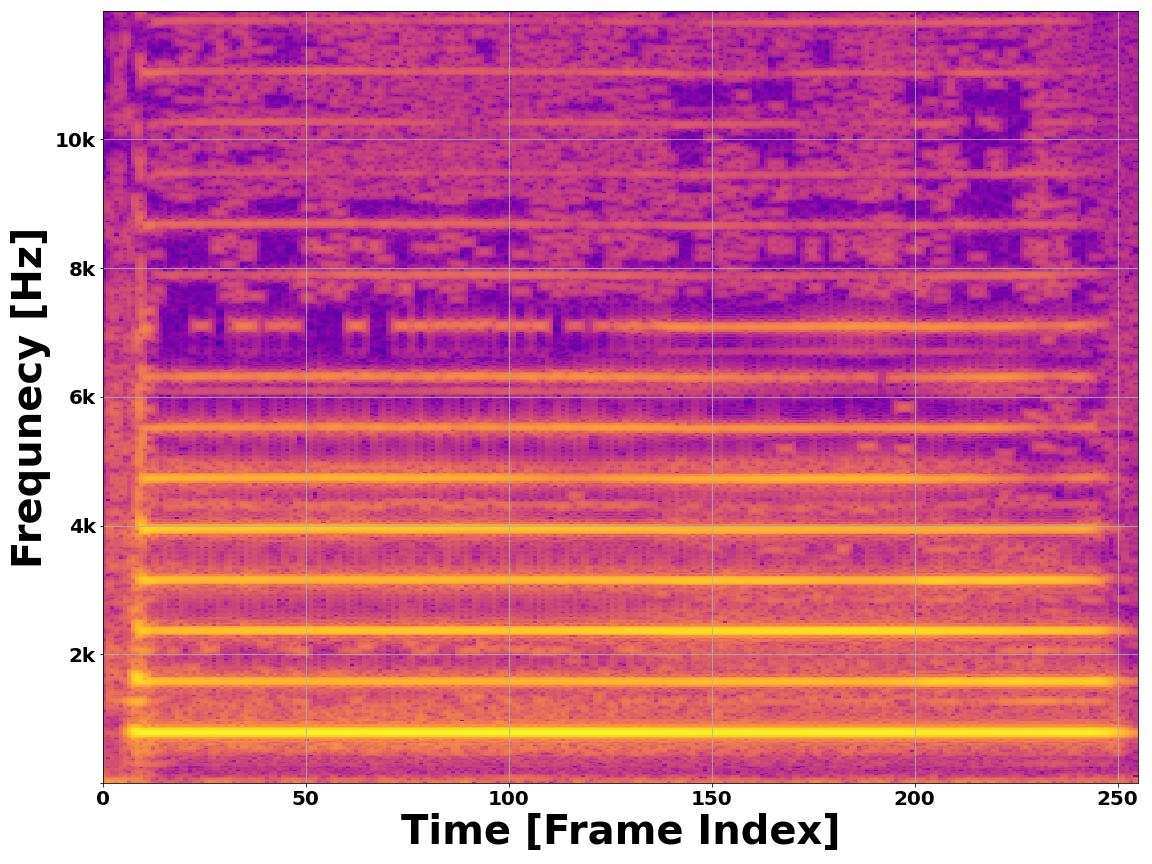
\includegraphics[scale=0.2]{../FiguresSpectrogram/Clarinet-Gs5}
	\caption{$B\flat$ Clarinet playing $G\sharp 5$}
	\end{subfigure}
	\hfill
	\begin{subfigure}[b]{0.45\textwidth}
	\centering
	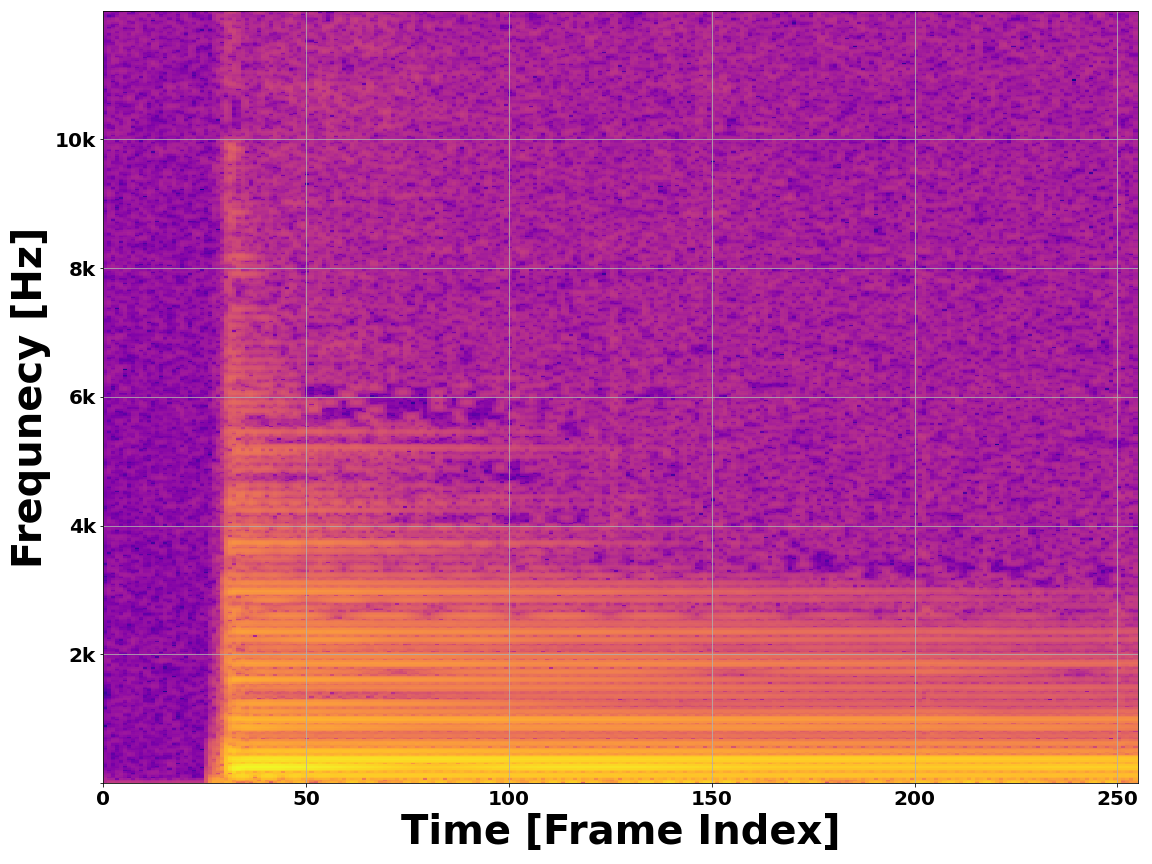
\includegraphics[scale=0.2]{../FiguresSpectrogram/GUITAR-B2}
	\caption{Guitar playing $B2$}
	\end{subfigure}
	
	\begin{subfigure}[b]{0.45\textwidth}
	\centering
	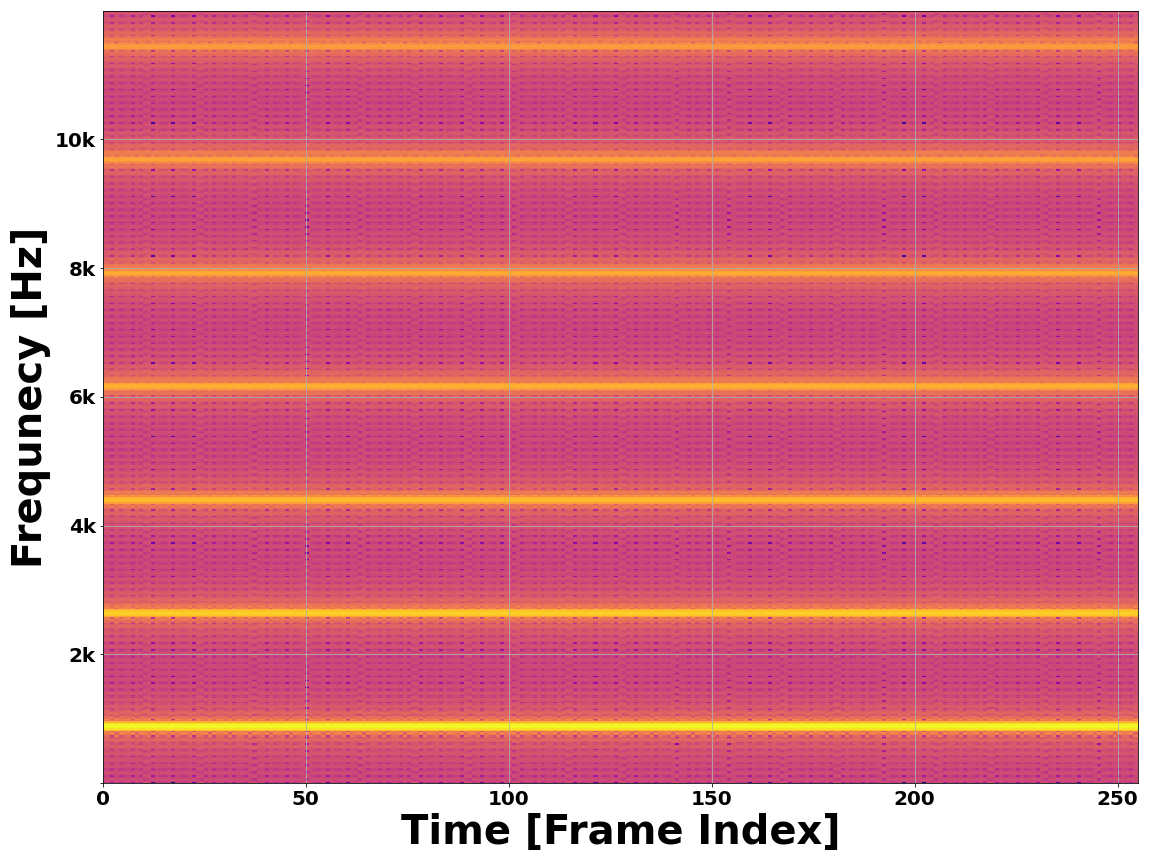
\includegraphics[scale=0.2]{../FiguresSpectrogram/SquareWave-880Hz}
	\caption{Square Wave at $880$ Hz}
	\end{subfigure}
	\hfill
	\begin{subfigure}[b]{0.45\textwidth}
	\centering
	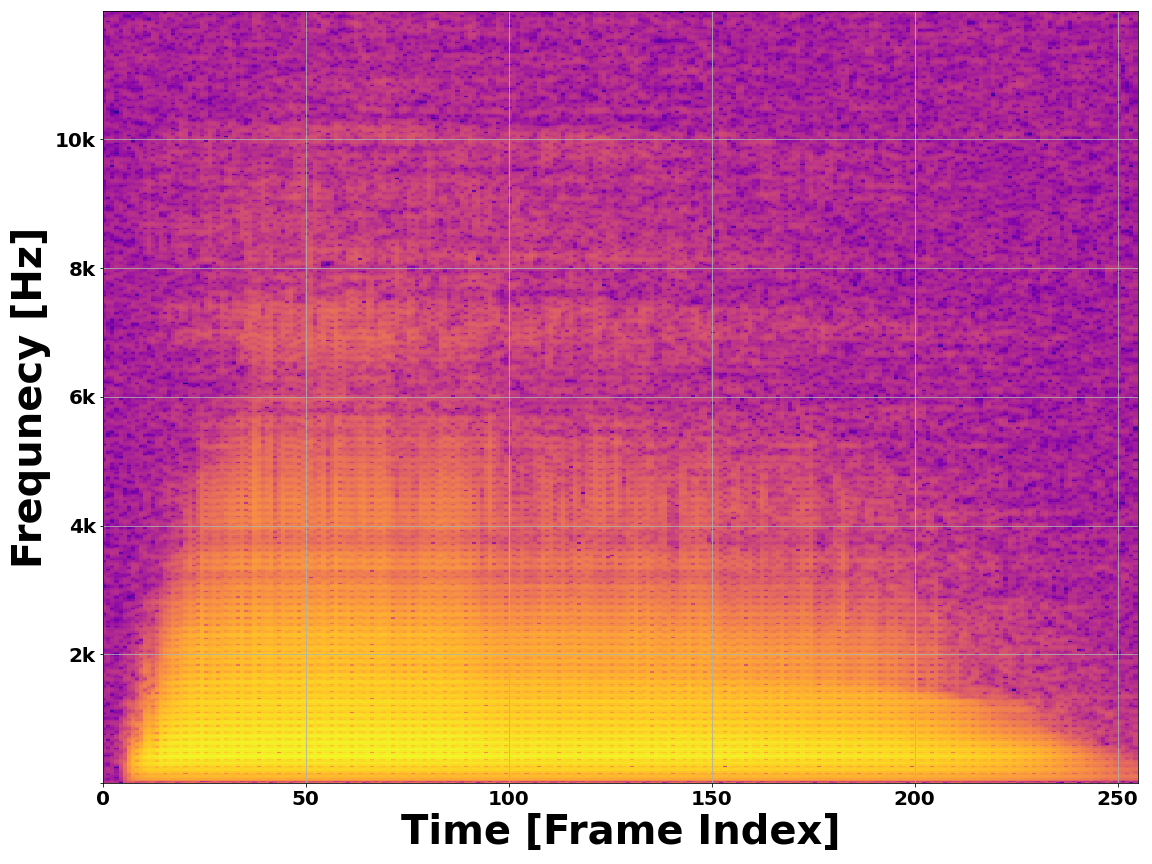
\includegraphics[scale=0.2]{../FiguresSpectrogram/Tuba-A2}
	\caption{Tuba playing $A2$}
	\end{subfigure}
\caption{Spectrogram representations of various waveforms. Note that all spectrograms are color-coded according to the log-power spectrum.}
\label{fig-Spectrograms}
\end{figure}

% ================================

\subsubsection{Frame Blocking}
\label{subsubsec-FrameBlocking}

\paragraph*{}A spectrogram is produced by the method of \textit{frame-blocking}, which is very prevalent in audio signal processing \cite{Liu,Zhang}. Frame-blocking takes a raw waveform or signal, $s$ and decomposes it into a set of analysis frames, $a_i$, with each being a fixed $N$ samples in length, and has a fixed overlap with the previous frame. Each of the $k$ frames then allows for a section of the signal to be analyzed in a \textit{quazi-stationary state} \cite{Khan,Serizel}. Below we visualize how analysis frames are related to the full time-series waveform. 

\begin{figure}[H]
\begin{center}
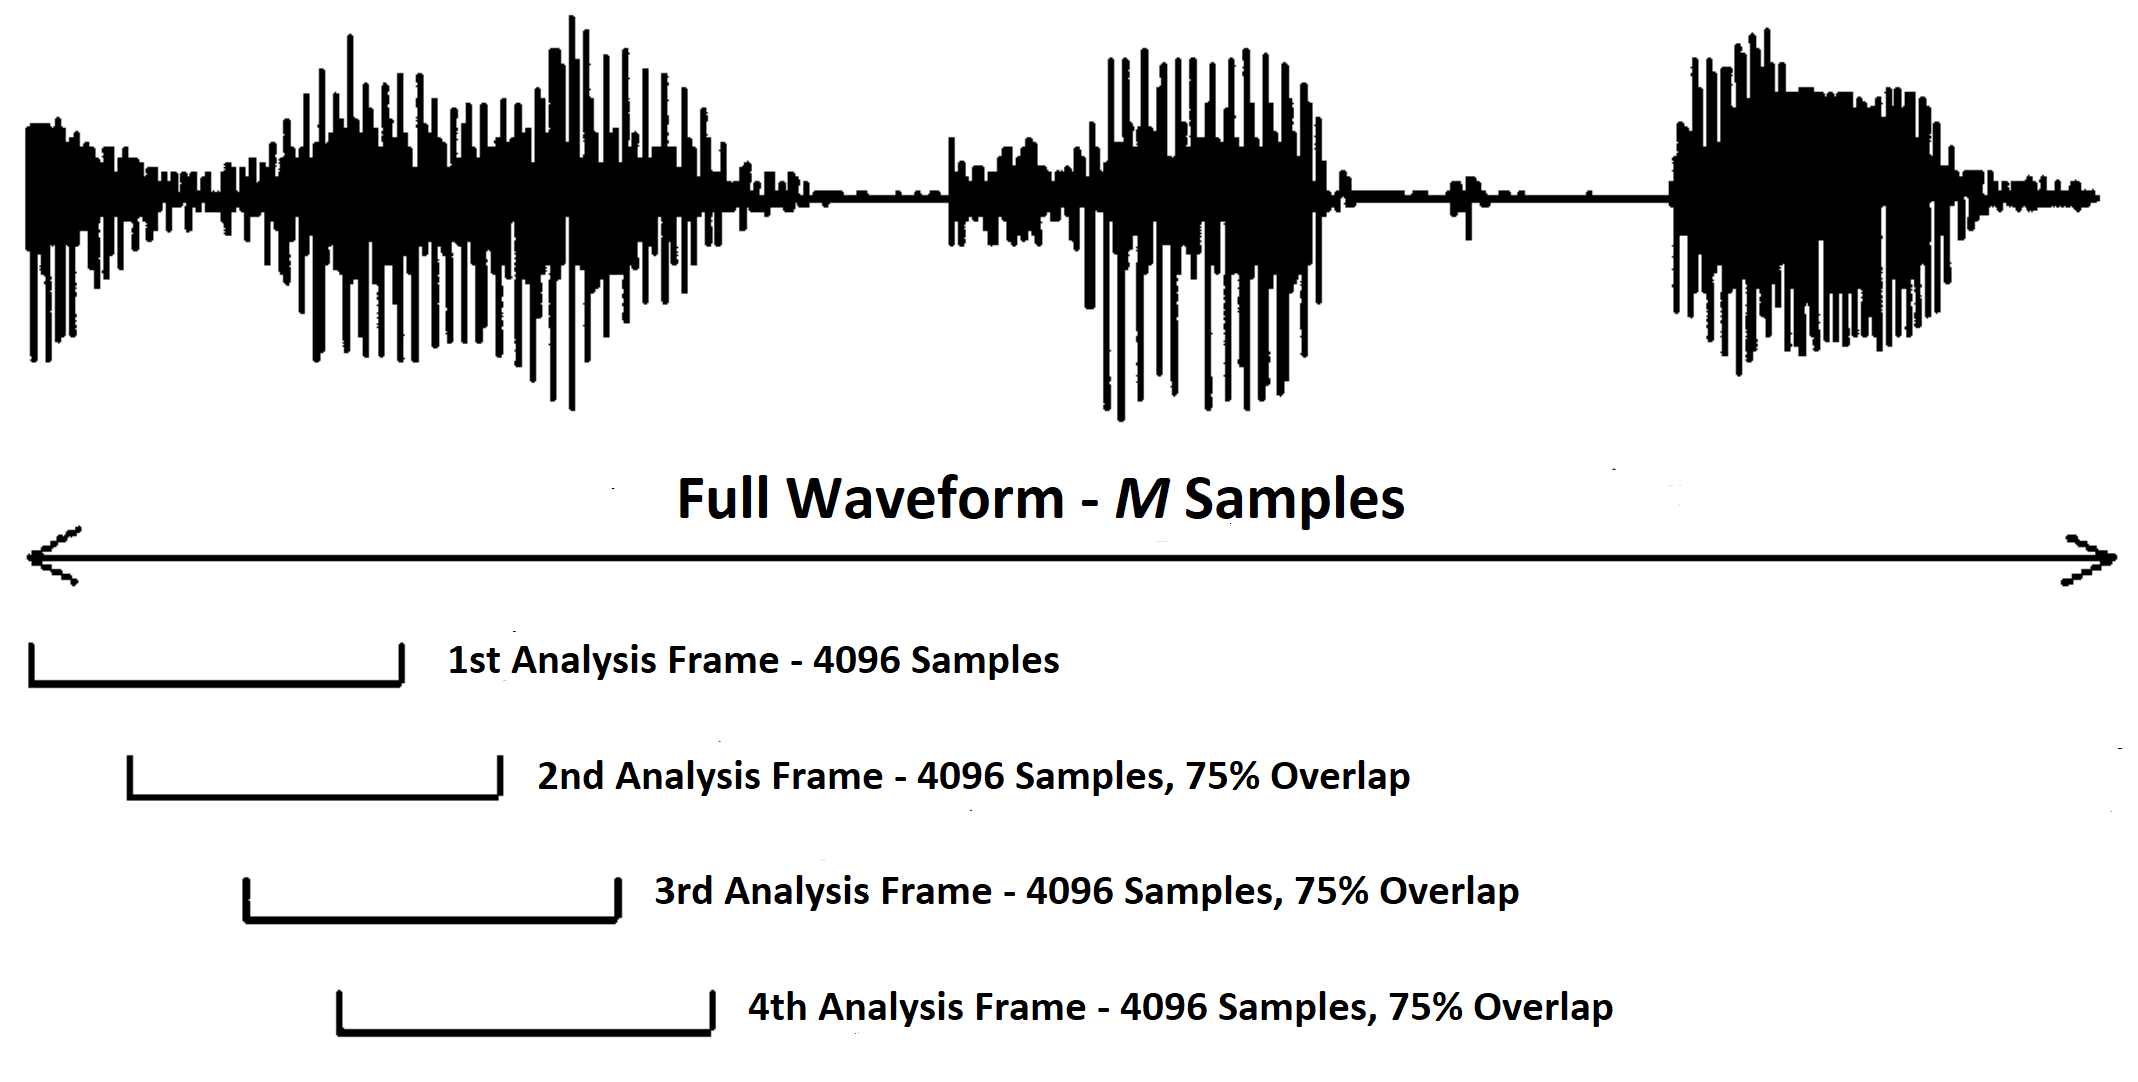
\includegraphics[scale=0.45]{../Figures/AnalysisFrames}
\end{center}
\caption{A visualization of how frame-blocking is used to create each analysis frames. This image has been adapted and modified from Liu, et. al. "Audio Feature Extraction and Analysis", Fig. (1). See ref. \cite{Liu}.}
\label{fig-AnalysisFrames}
\end{figure}

\paragraph*{}For this project, we have chosen to use frames of size $N = 1024$ with a $75\%$ or $768$ sample overlap. Since each audio file contains a different number of samples, we choose the number of frames, $k$ to be less than or equal to $256$. If $k > 256$, the waveform in truncated, if $k \leq 256$ the frames left as is, and missing frames are accounted for later (to improve computation time). The audio has been sampled at $f_s = 44100$ samples/second, so each frame represents a slice of time that is about $0.0232$ seconds long.

\paragraph*{}We concatenate each analysis frame, $a_{i}, i \in [0,k-1]$ into a single $k \times N$ matrix, called $A$. Each row is a frame, each column is a sample in each frame
\begin{equation}
\label{eqn-FrameMatrix}
A = \big\{ a_{0} , a_{1} , a_{2} , ... , a_{k-1} \big\} = 
\begin{bmatrix}
a_{0}[0] & a_{0}[1] & a_{0}[2] & \hdots & a_{0}[N-1] \\
a_{1}[0] & a_{1}[1] & a_{1}[2] & \hdots & a_{1}[N-1] \\
a_{2}[0] & a_{2}[1] & a_{2}[2] & \hdots & a_{2}[N-1] \\
\vdots 		& \vdots 	  & \vdots 		& \ddots & \vdots        \\
a_{k-1}[0] & a_{k-1}[1] & a_{k-1}[2] & \hdots & a_{k-1}[N-1] \\
\end{bmatrix}
\end{equation}
We use bracket notation, $a_i[j]$ to indicate that each analysis frame $a_i$ is array-like. The following indexing conventions for matrix $A$ all represent the same entry:
\begin{equation}
\label{eqn-IndexingA}
A_{i,j} = A_i[j] = A[i,j]
\end{equation}

% ================================

\subsubsection{Windowing}
\label{subsubsec-Windowing}

\paragraph*{}After frame-blocking, we apply a \textit{windowing function} to each frame. A standard \textit{Hanning Window} of $N$ samples is generated as a $1 \times N$ row-array, $H$. The $n$-th index in a Hanning window with $N$ samples is defined:
\begin{equation}
\label{eqn-Hanning}
H[n] = \frac{1}{2}\bigg[ 1 - \cos\Big( \frac{2\pi n}{N-1}\Big)\bigg]
\end{equation}
This window function is applied to each analysis frame by computing the element-wise product of the Hanning window array, $H$ and each row of the analysis frames matrix, $A[i,:]$. The result is another $k \times N$ array, which is denoted as $\widetilde{A}$, and is given by:
\begin{equation}
\label{eqn-WindowMatrix}
\widetilde{A_i} = A_i \odot H
\end{equation}
We show the effect of a Hanning window applied to an analysis frame:
\begin{figure}[H]

	\begin{subfigure}{1.0\textwidth}
	\centering
	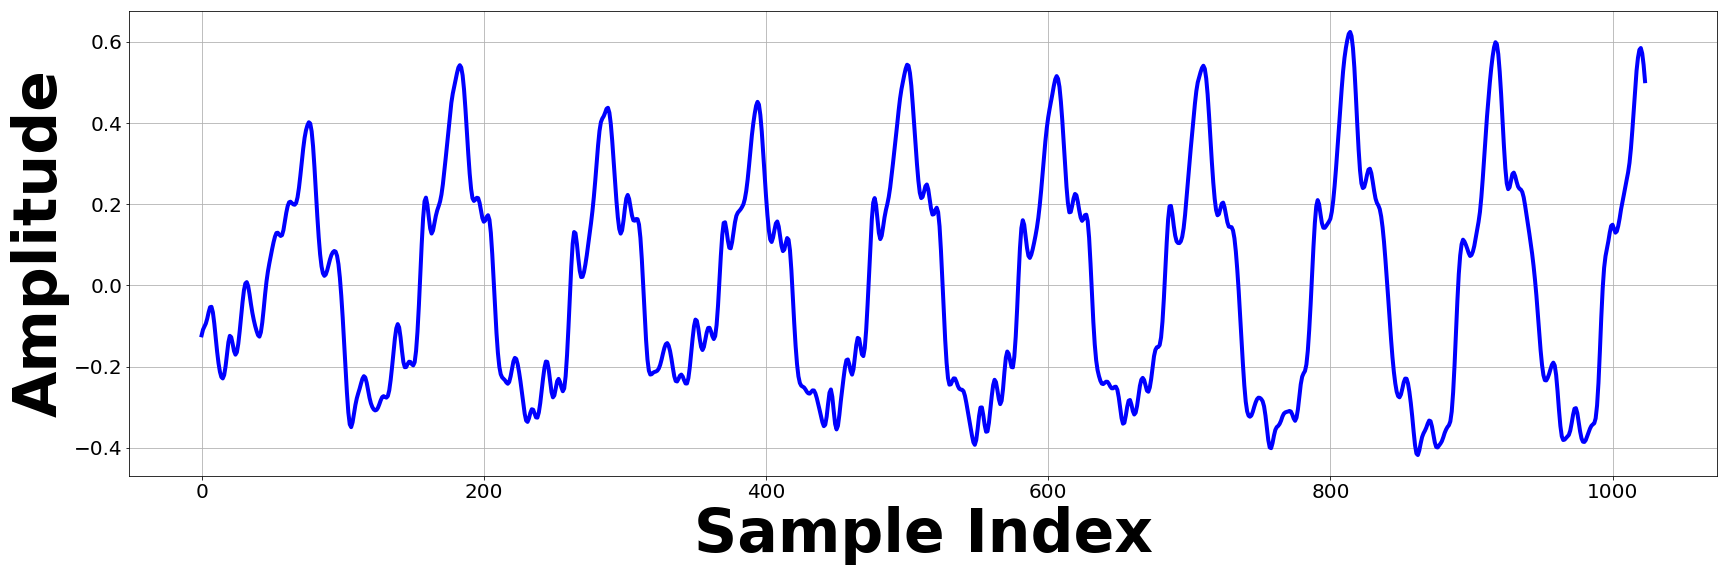
\includegraphics[width=\textwidth , height=0.2\textheight]{../Figures/AnalysisFrame}
	\caption{A section of a violin bowing an $A4$ note, $1024$ samples long}
	\end{subfigure}	
	
	\begin{subfigure}{1.0\textwidth}
	\centering
	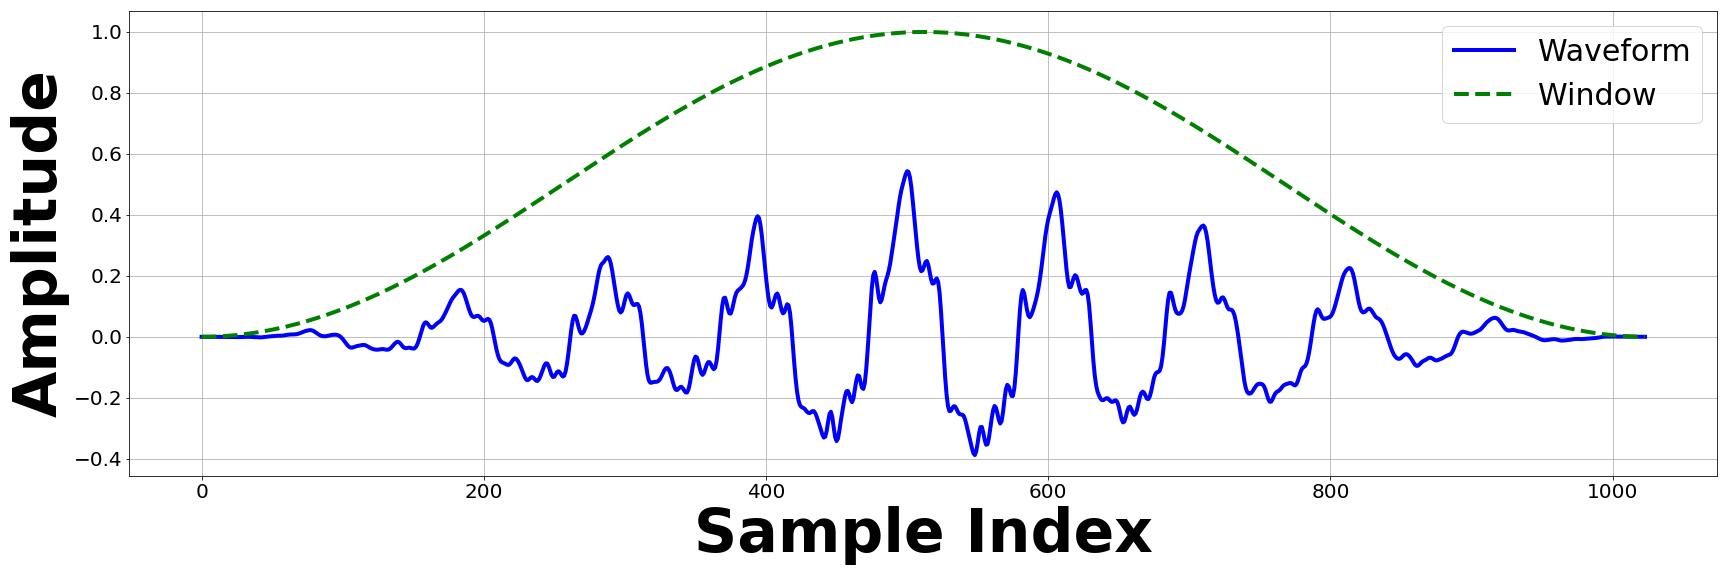
\includegraphics[width=\textwidth , height=0.2\textheight]{../Figures/WindowedFrame}
	\caption{The same waveform with a Hanning Window Applied}
	\end{subfigure}	

\end{figure}

\paragraph*{}Window functions are use to account for discontinuities that may arise in the waveform at the edges of each analysis frame. The Fourier Transform assumes that an integer number of signal periods fit within each analysis frame, however this is rarely the case. Transforming a signal with to \textit{spectral leakage} where energy appears to "leak" into adjacent frequency bins. This result is a frequency domain that is not an accurate representation of the equivalent time domain. The Hanning window uses the raised cosine function to taper the signal off to zero at the end-points, thus eliminate discontinuities at the edges while weighting the samples at the center much more heavily. This allows for a much cleaner transform into frequency space.

\paragraph*{}Before we compute the Fourier Transform to move each analysis frame into frequency-space, we choose to tail-pad each analysis frame with an additional $1024$ samples of all zeros. This means that each frame has gone from being $1024$ samples, to $2048$ samples. Matrix $\widetilde{A}$ has a shape of $k \times 2048$. Doubling the size of each analysis frame allows us the synthetically double the resolution in frequency-space, while retaining the resolution in time-space \cite{Virtanen}. 

% ================================

\subsubsection{Discrete Fourier Transform}
\label{subsubsec-DFT}

\paragraph*{}With this final change, we perform a \textit{Discrete Fourier Transform} (DFT) to bring each analysis frame from a time domain into a frequency domain \cite{Olson,Peatross,Virtanen}. The Discrete Fourier Transform is applied by producing an $N \times N$ \textit{transform matrix}, often noted as $\mathbb{W}$. Let $\omega^k = e^{\frac{-2\pi i}{N}k}$, then the DFT matrix for a time-space signal containing $N$ samples is given by \cite{Taylor,Peatross,Virtanen}:
\begin{equation}
\label{eqn-DFTMatrix}
\mathbb{W} = 
\begin{bmatrix}
1 & 1 & 1 & 1 & \hdots & 1 \\
1 & \omega		& \omega^2 & \omega^3 & \hdots & \omega^{N-1} \\
1 & \omega^2	& \omega^4 & \omega^6 & \hdots & \omega^{2(N-1)} \\
1 & \omega^3	& \omega^6 & \omega^9 & \hdots & \omega^{3(N-1)} \\
\vdots & \vdots & \vdots & \vdots & \ddots & \vdots \\
1 & \omega^{N-1} & \omega^{2(N-1)} & \omega^{3(N-1)} & \hdots & \omega^{(N-1)^2}
\end{bmatrix}
\end{equation}
Each column of the matrix is a complex sinusoidal oscillating with an integer number of periods within the $N$-sample length window \cite{Short,Peatross}. The DFT is applied by a taking the matrix - product of $\mathbb{W}$ and $\widetilde{A}^T$. The transpose of $\widetilde{A}$ makes each analysis frame into a column vector, which gives the appropriate format for transformation.
\begin{equation}
\label{eqn-DFT}
\text{DFT}\big[ \widetilde{A} \big] = \mathbb{W}\widetilde{A}^T
\end{equation}

\paragraph*{}Most standard implementations of neural network models use activations, weights, and biases to all be real floating-point numbers \cite{Levine,Loy,Tensorflow}. Since the elements of the DFT matrix lie on the complex unit circle, each real-valued analysis frame will be moved into complex space. This means we compute the element-wise product of the transformed signal matrix and it's complex-conjugate matrix. This is the $N \times k$
spectrogram matrix, where each element is a real-values number. Matrix $S$ is defined:
\begin{equation}
\label{eqn-Spectrogram}
S = (\mathbb{W}\widetilde{A}^T) \odot (\mathbb{W}\widetilde{A}^T)^*
\end{equation}
Where $\mathbb{W}$ is the DFT matrix from Eq. (\ref{eqn-DFTMatrix}) and $\widetilde{A}^T$ is the transpose of the analysis frames matrix from Eq. (\ref{eqn-WindowMatrix}). The asterisks indicate the element-wise complex conjugation. In practice, the matrix product $\mathbb{W}\widetilde{A}^T$ is computed once, and the conjugate is applied to a copy of the array.

\paragraph*{}The matrix $S$, is the spectrogram representation of the initial waveform, and has shape $N \times k$ of all real floating-point numbers. We can index matrix $S$ similarly to that of matrix $A$ in Eq. (\ref{eqn-IndexingA}):
\begin{equation}
\label{eqn-IndexingS}
S_{i,j} = S_i[j] = S[i,j]
\end{equation}
Note that the spectrogram provided to the neural network is representing the power spectrum of the audio file as defined in Eq. (\ref{eqn-Spectrogram}). All spectrogram figures in this report are from taking the element-wise \textit{natural log} of the power spectrum. This has been done solely for visualization purposes.

\paragraph*{}Each column of the $S$ matrix is now a single analysis frame that has been moved into a frequency-space representation of itself. There are $k$ columns, just as there were $k$ time-series frames, and $N$ rows since there were $N$ samples per row. Given the discrete nature of digital audio, the frequency-space representation is not a continuous function, but rather a column vector, where the frequency has been assigned to one of $N$ bins, ranging from $-f_s / 2$ to $+f_s/2$ \cite{Short,Peatross}. To ensure homogeneous input sizes between all samples, we zero-pad the matrix $S$ with additional columns until $k = 256$, which mimics tail-padding the original signal with zeros. Recall that wave forms were truncated to ensure that $k \leq 256$ analysis frames.

\paragraph*{}Standard western musical instruments seldom have fundamental frequencies that extend above $6$ kHz \cite{Olson,Virtanen,White}. This means that when constructing the spectrogram, we will rarely see significant energy present above $12$ kHz at any time, and the $S$ matrix will contain mostly zero, or zero-like entries. To condense the size of the matrix, we select only the frequency bins (rows) that correspond to energies between $0$ Hz and $12,000$ Hz. This makes the input array smaller, (less than 1/4 the size) and eliminates redundant and non-useful information. The number rows in the $S$ matrix is reduced from $N$ down to $N'$. 

\paragraph*{}Each spectrogram is now $N' \times k$ and effectively encodes the energy distribution of the waveform as a function of both time and frequency. The spectrogram makes up each sample in the first design matrix $X_1$, Eq.(\ref{eqn-X1Shape}) used in this model. For this classifier, we have chosen $N' = 558$ and $k = 256$. For training, a batch of $b$ samples are concatenated into a single array object. For a batch of $b$ samples of $N' \times k \times 1$ spectrograms, we shape $X_1$ such that:
\begin{equation}
\label{eqn-X1}
X_1 = \big\{ S^{(0)},S^{(1)},S^{(2)}, ... , S^{(b-1)} \big\} \in \mathbb{R}^{(b \times N' \times k \times 1)}
\end{equation}
Which is consistent with the shape of the $X_1$ matrix outlined in Eq. (\ref{eqn-X1Shape}). This matrix is presented to the \textit{Convolution} branch of the neural network for processing.

% ================================================================

\subsection{Time-Space Features}
\label{subsec-TimeFeatures}

\paragraph*{}The features described in this section are derived from time-domain representations of each audio sample.  For consistency between samples, each waveform is padded or truncated to contain the same number of samples $M$. The number of samples $M$ is chosen to correspond the same number of samples as needed to make the $N \times k$ spectrogram matrix. In doing this, the spectrogram and time-series features are representative of the same time interval in the file sample. Time space is indexed by $s[i]$ with $i \in [0,1,2,3,...,M-2,M-1]$

\paragraph*{}From time space, we use the following $11$ features:
\begin{itemize}
\item[•] Time Domain Envelope ($\times 5$)
\item[•] Zero Crossing Rate
\item[•] Temporal Center of Mass
\item[•] Auto Correlation Coefficients ($\times 4$)
\end{itemize}

% ================================

\subsubsection{Time Domain Envelope}

\paragraph*{}The time domain envelope (TDE) is a rough measurement of the energy contained in the time-space of the waveform. If we divide the signal into analysis frames, as in Fig. (\ref{fig-AnalysisFrames}), then the TDE approximates the energy in that frame. A frame with a high TDE indicates a generally large amplitude, and a frame with a low TDE indicates a generally small amplitude, i.e. the signal has not started or is decaying. The small size of each analysis frame makes computing a TDE for each impractical, and creates a very high-dimensional feature vector. This would also cause problems as some waveforms may have an initial attack that differs in time by a few analysis frames. Computing TDE for each frame would therefore introduce temporal bias, as the same waveform delayed by a few milliseconds would generate a slightly different set of predictor values \cite{Serizel}. 

\paragraph*{}One way to mitigate this is to group analysis frames together and compute the TDE of a collection of frames. This way,  almost all waveforms will produce an identical set of features to a short time-delayed version of itself. By choosing a sufficiently large number of TDE values, we can also generate an approximation of than amplitude envelope of the time-series waveform. This comes at a higher computational cost, and a previously mentioned higher dimensional feature vector

\paragraph*{}We adapt this TDE to \textbf{compute the time domain envelope over $5$ non-overlapping analysis frames}. Since the maximum amplitude of each waveform array has been normalized to $\pm 1$, the TDE represents a consistent measurement of energy in each waveform subset \cite{Liu}. The TDE is computed as the RMS-Energy of the waveform, $s$ and the $j$-th TDE value is given by \cite{Olson,Serizel}:
\begin{equation}
\label{eqn-RMS}
\text{TDE}_j\big[ s \big] = \sqrt{\frac{1}{Q} \sum_{i=n}^{n+Q} s[i]^2}
\end{equation}
Where $Q$ gives the number of samples in each analysis frame (number of sample sin waveform divided by number of frames), and $n$ gives the index where the $j$-th frame begins. We provide a graphic representation of how the TDE compares to the amplitude of sections of a waveform in Fig. (\ref{fig-ExampleTDE}).

\begin{figure}[H]
	\begin{subfigure}[b]{0.45\textwidth}
	\begin{center}
	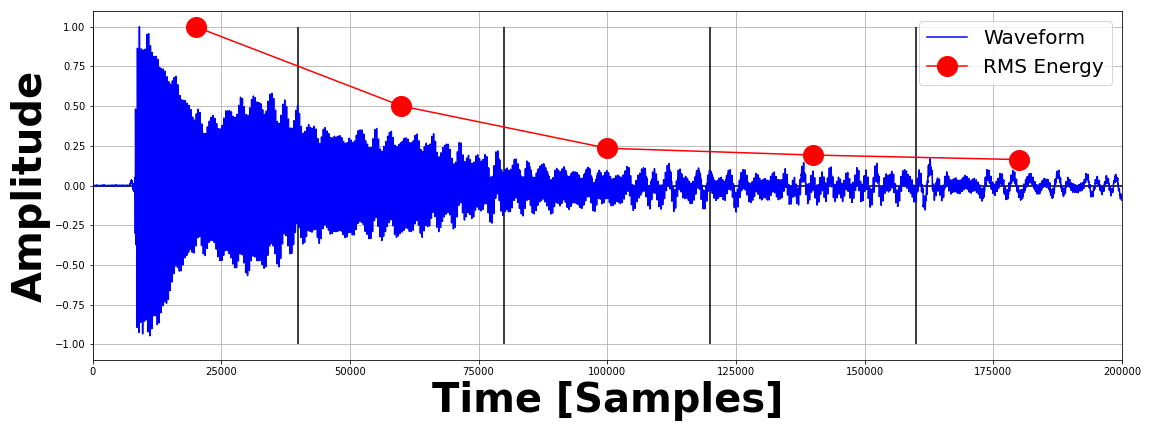
\includegraphics[width=1.0\linewidth]{../FiguresSpectrogram/GUITAR-B2_TDE}
	\caption{Guitar - B2}
	\end{center}
	\end{subfigure}	
	\hfill
	\begin{subfigure}[b]{0.45\textwidth}
	\begin{center}
	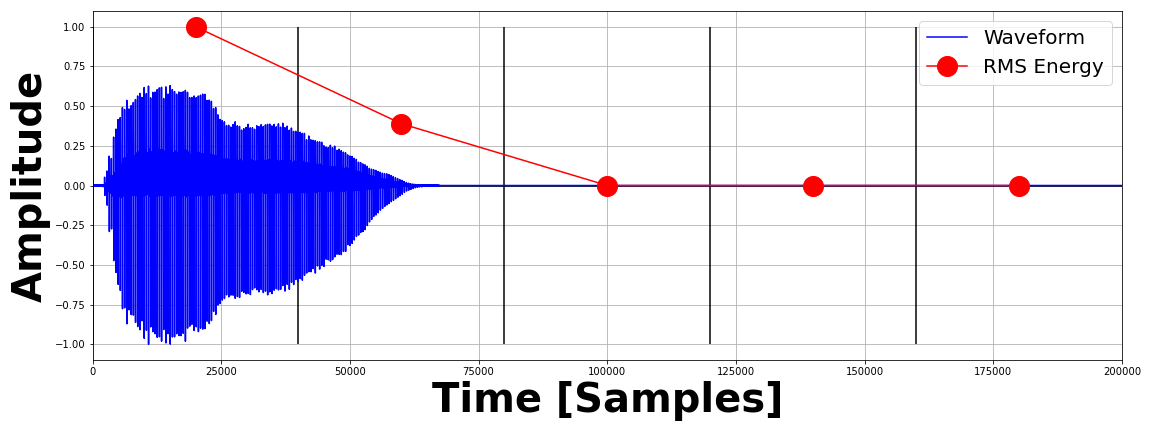
\includegraphics[width=1.0\linewidth]{../FiguresSpectrogram/Tuba-A2_TDE}
	\caption{Tuba - A2}
	\end{center}
	\end{subfigure}
	\caption{TDE Envelope values for musical instruments}
	\label{fig-ExampleTDE}
\end{figure}

\paragraph*{}The uniformly sized analysis frames let us create an naive envelope of the waveform, but will allow it to generalize between classes. For example, this allows for a crude approximation of the energy in the attack, decay, sustain, and release portion of the signal \cite{Virtanen,Olson}. For instruments with heavier attacks, we expect the TDE in the first frame to be comparably large, see Fig. (\ref{fig-FeatureTDE}a). Instruments with a heavy decay will likely have little energy in the second or higher frames, indicating that the amplitude has substantially died off as in Fig. (\ref{fig-FeatureTDE}b). Conversely, instruments with longer sustain such as upper woodwinds, vibraphones or strings will contain relatively higher TDE values for the later analysis frames as seen in Fig. (\ref{fig-FeatureTDE}c). Instruments with little or no waveform envelope, such as the synthesized waveforms and the whitenoise show constant TDE values across each frame as expected.

\begin{figure}[H]

	\begin{subfigure}{1.0\textwidth}
	\centering
	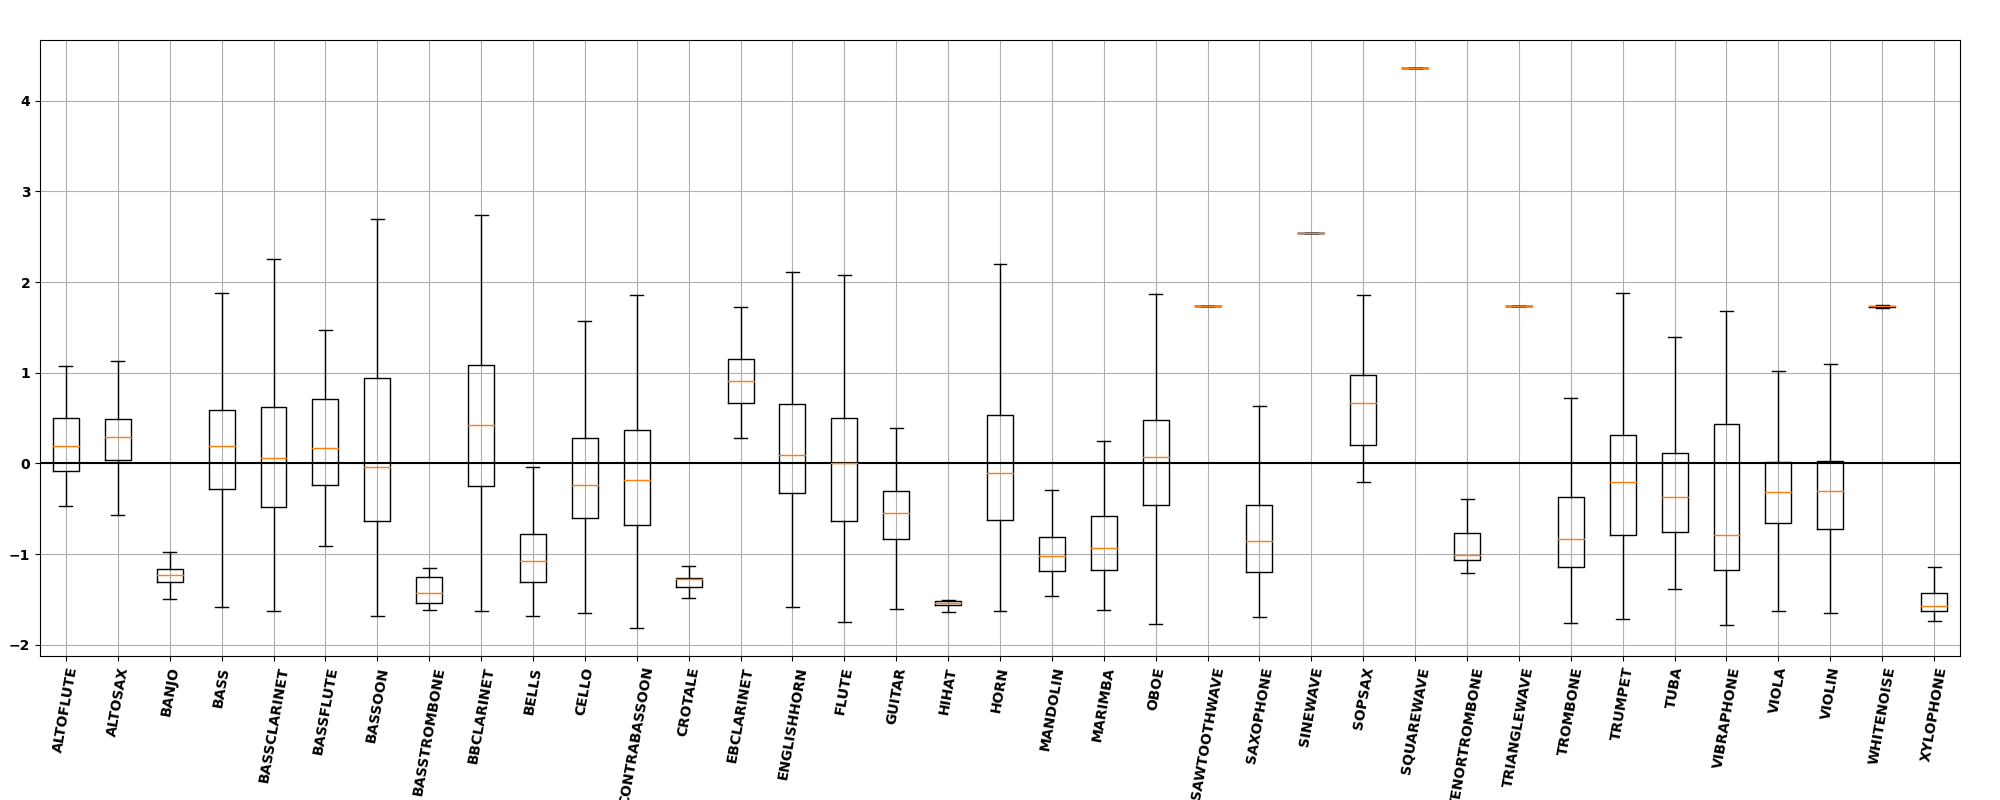
\includegraphics[width=\textwidth , height=0.2\textheight]
		{../FiguresFeatures/TDE_1}
	\caption{TDE $1$}
	\end{subfigure}
	
	\begin{subfigure}{1.0\textwidth}
	\centering
	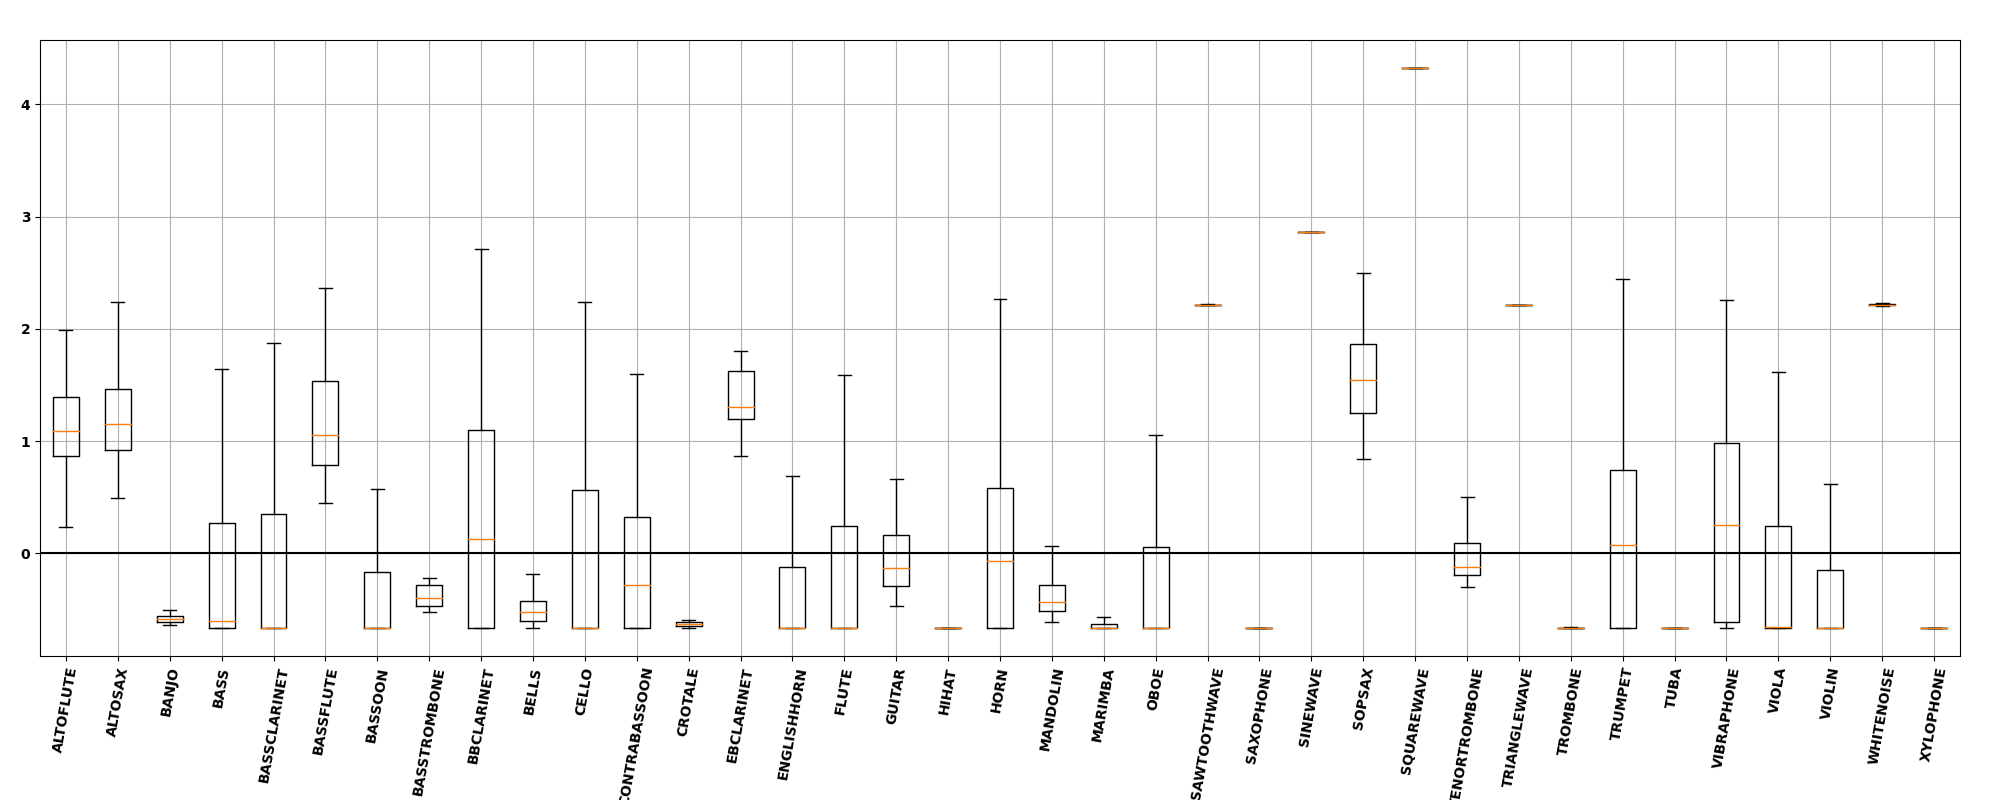
\includegraphics[width=\textwidth , height=0.2\textheight]
		{../FiguresFeatures/TDE_2}
	\caption{TDE $2$}
	\end{subfigure}
	
	\begin{subfigure}{1.0\textwidth}
	\centering
	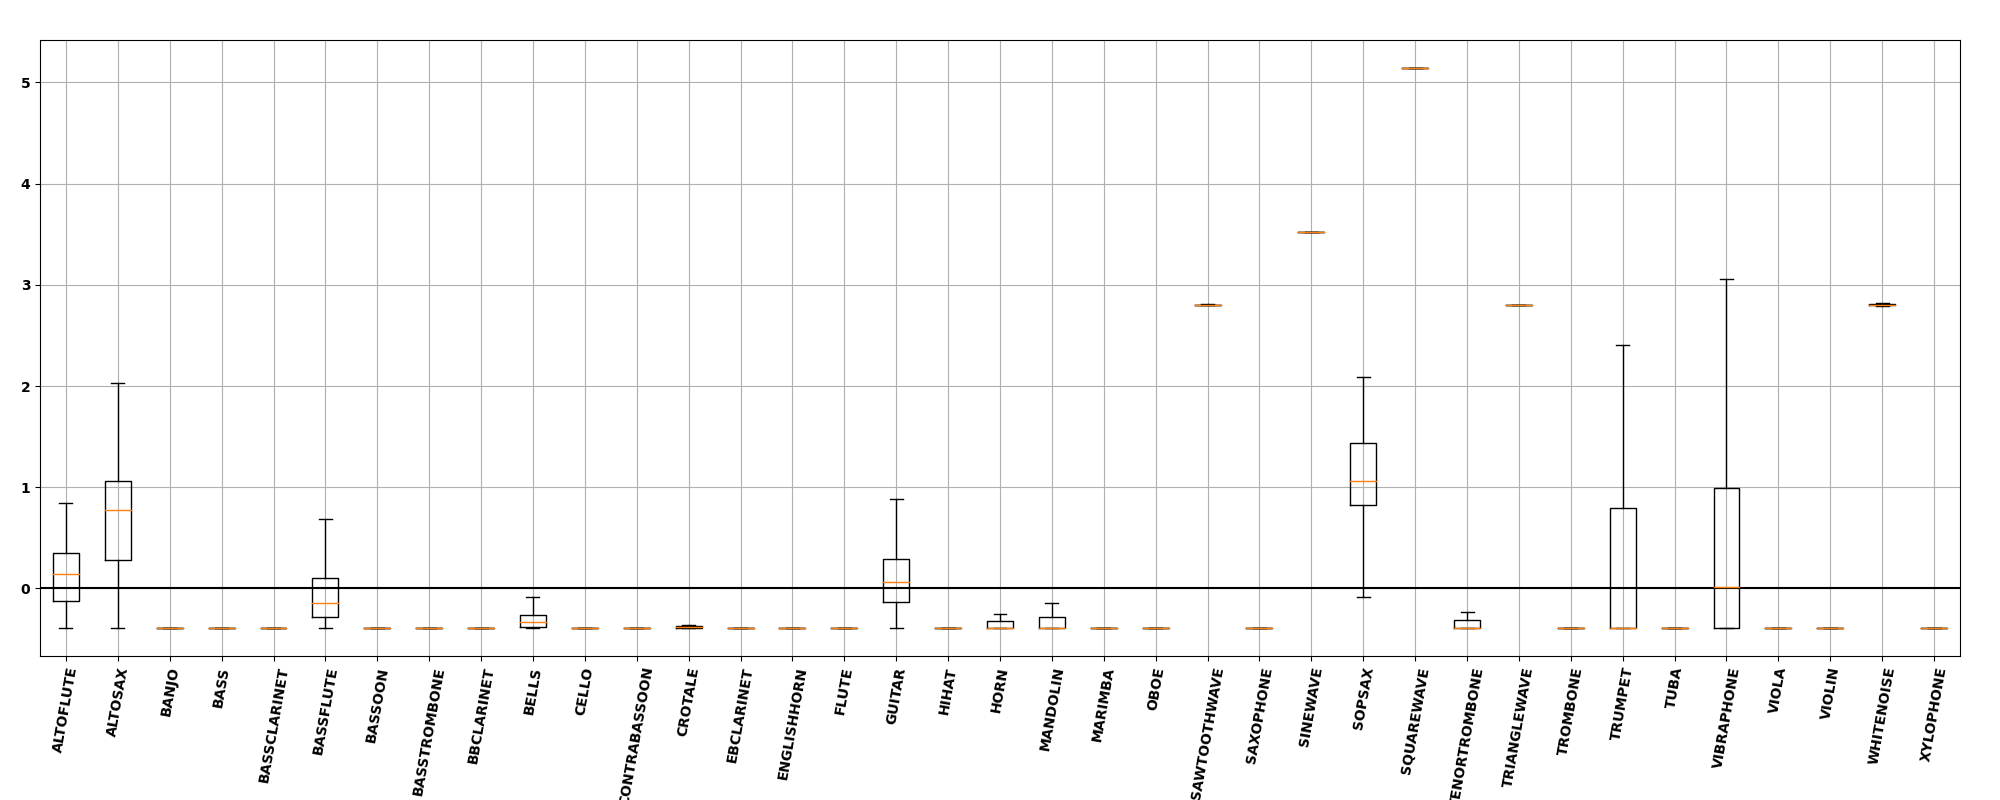
\includegraphics[width=\textwidth , height=0.2\textheight]
		{../FiguresFeatures/TDE_3}
	\caption{TDE $3$}
	\end{subfigure}
		
\caption{A comparison of the first three of five time domain envelope values across each class using a box-and-whisker plot}
\label{fig-FeatureTDE}
\end{figure}

% ================================

\subsubsection{Zero Crossing Rate}

\paragraph*{}The zero crossing rate (ZXR) of a signal or frame is use to measure how many times that a signal crosses it's equilibrium point. This can be computed per total sound wave, per analysis-frame, or per unit time. This feature is most commonly associated with differentiating speech from music, because speech presents a more jagged and often less periodic waveform that musical instruments do \cite{Khan,Liu,Zhang} . 

\paragraph*{}We adapt this feature to \textbf{compute the zero crossing rate for the full waveform}. Signals with a high ZXR can be representative of classes that often have additional noise and signals with a low ZXR, can indicate signals with more stable, periodic behavior. The ZXR for the full waveform $s$ is given by \cite{Serizel,Liu}
\begin{equation}
\label{eqn-ZXR}
\text{ZXR}\big[ s \big] = \frac{1}{2} \sum_{i=1}^{M-1} \Big{|} \sign(s[i]) - \sign(s[i-1]) \Big{|} 
\end{equation}
Where $\sign(x)$ returns $+1$ if $x > 0$, $-1$ if $x < 0$ and $0$ if $x = 0$. ZXR also provides a very rough estimate for the average frequency of the waveform. This allows it to allows be useful in discerning classes with generally higher fundamental frequencies, such as upper woodwinds, against classes with generally lower frequencies, such as low brass \cite{Liu,White}.

\paragraph*{}This behavior becomes apparent when comparing sets of classes in Fig. (\ref{fig-FeatureZXR}). For example, consider the ZXR value of a a bass and cellos against that of bells or a soprano saxophone. The bass and cellos have on average much lower fundamental frequencies than that of cellos of soprano saxophones. In the case of this data set, the ZXR provides a predictor which contains clear separations between classes such as crotales and $E\flat$ clarinets. 
\begin{figure}[H]
\begin{center}
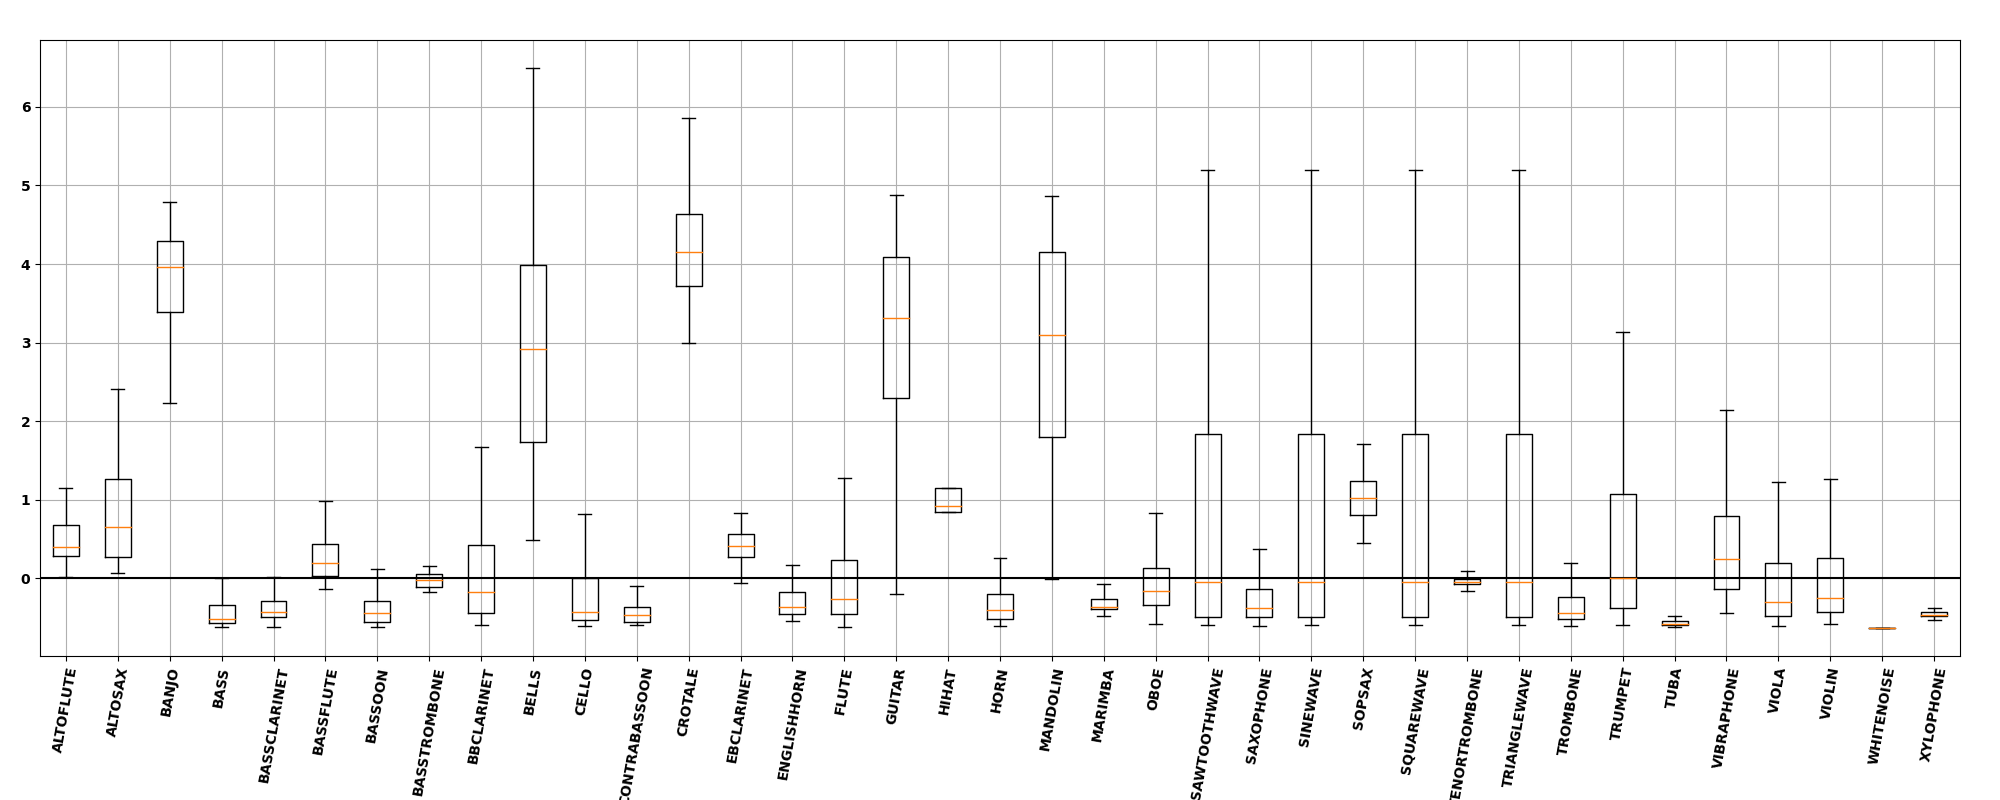
\includegraphics[scale=0.3]{../FiguresFeatures/ZXR}
\end{center}
\caption{A comparison of the zero-crossing rate for each class using a box-and-whisker plot}
\label{fig-FeatureZXR}
\end{figure}

% ================================

\subsubsection{Temporal Center of Mass}

\paragraph*{}The temporal center of mass (TCM) of a signal is used to compute roughly where in time the amplitude of the waveform \textit{bunches up}. We compute the element-wise absolute value of the waveform and treat it as a 1-dimensional discrete mass distribution of $M$ samples.
The TCM of that waveform is then given:
\begin{equation}
\label{eqn-FeatureTCM}
\text{TCM}\big[ s \big] = \frac{\sum_{i=0}^{M-1}i \big|s[i]\big|}
{\sum_{i=0}^{M-1}\big|s[i]\big|}
\end{equation}

\paragraph*{}TCM condenses the idea of the amplitude envelope into a single scalar value. It allows for the quick measurement of where in the time most of the energy of the signal lies. For percussive instruments with short attack and release times, such as bells or xylophones, we expect a very low TCM. Instruments with plucked strings, but longer release times such as mandolins and guitars should have similarly low values. See Fig. (\ref{fig-ExampleTCM}) for examples.
\begin{figure}[H]
	\begin{subfigure}[b]{0.45\textwidth}
	\begin{center}
	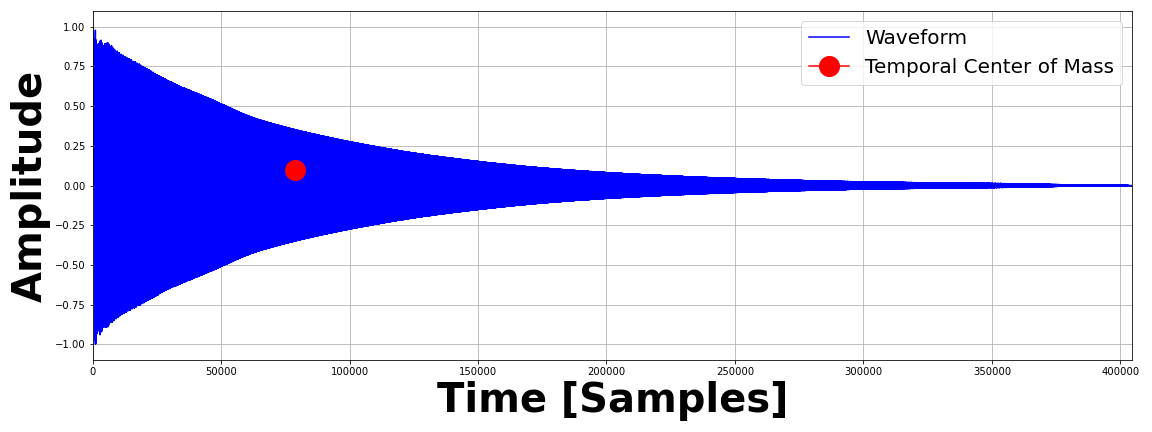
\includegraphics[width=1.0\linewidth]{../FiguresSpectrogram/Vibraphone-sustain-A5-R_TCM}
	\caption{Vibraphone at $A5$ shows a lower TCM}
	\end{center}
	\end{subfigure}	
	\hfill
	\begin{subfigure}[b]{0.45\textwidth}
	\begin{center}
	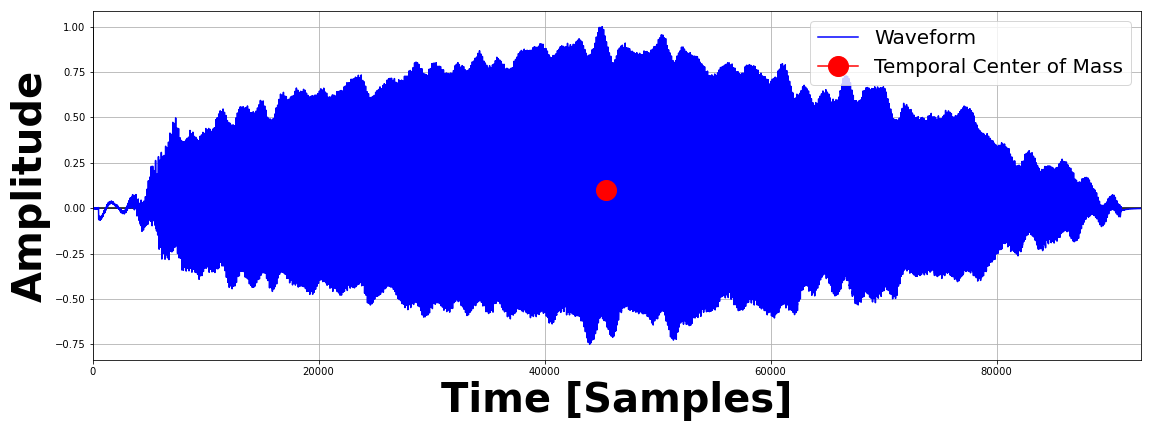
\includegraphics[width=1.0\linewidth]{../FiguresSpectrogram/CELLO-F4_TCM}
	\caption{Cello at $F4$ shows a central TCM}
	\end{center}
	\end{subfigure}
	\caption{TCM values for musical instruments}
	\label{fig-ExampleTCM}
\end{figure}
Instruments in the woodwind and brass family generally have longer sustain and release times, giving them a slightly higher center of mass. Strings and undampened percussion have notoriously long sustain and release times giving them much higher TCM values \cite{Olson,White}. Finally, the synthetic wave forms have no characteristic envelope shape which gives a centrally located TCM.

\begin{figure}[H]
\begin{center}
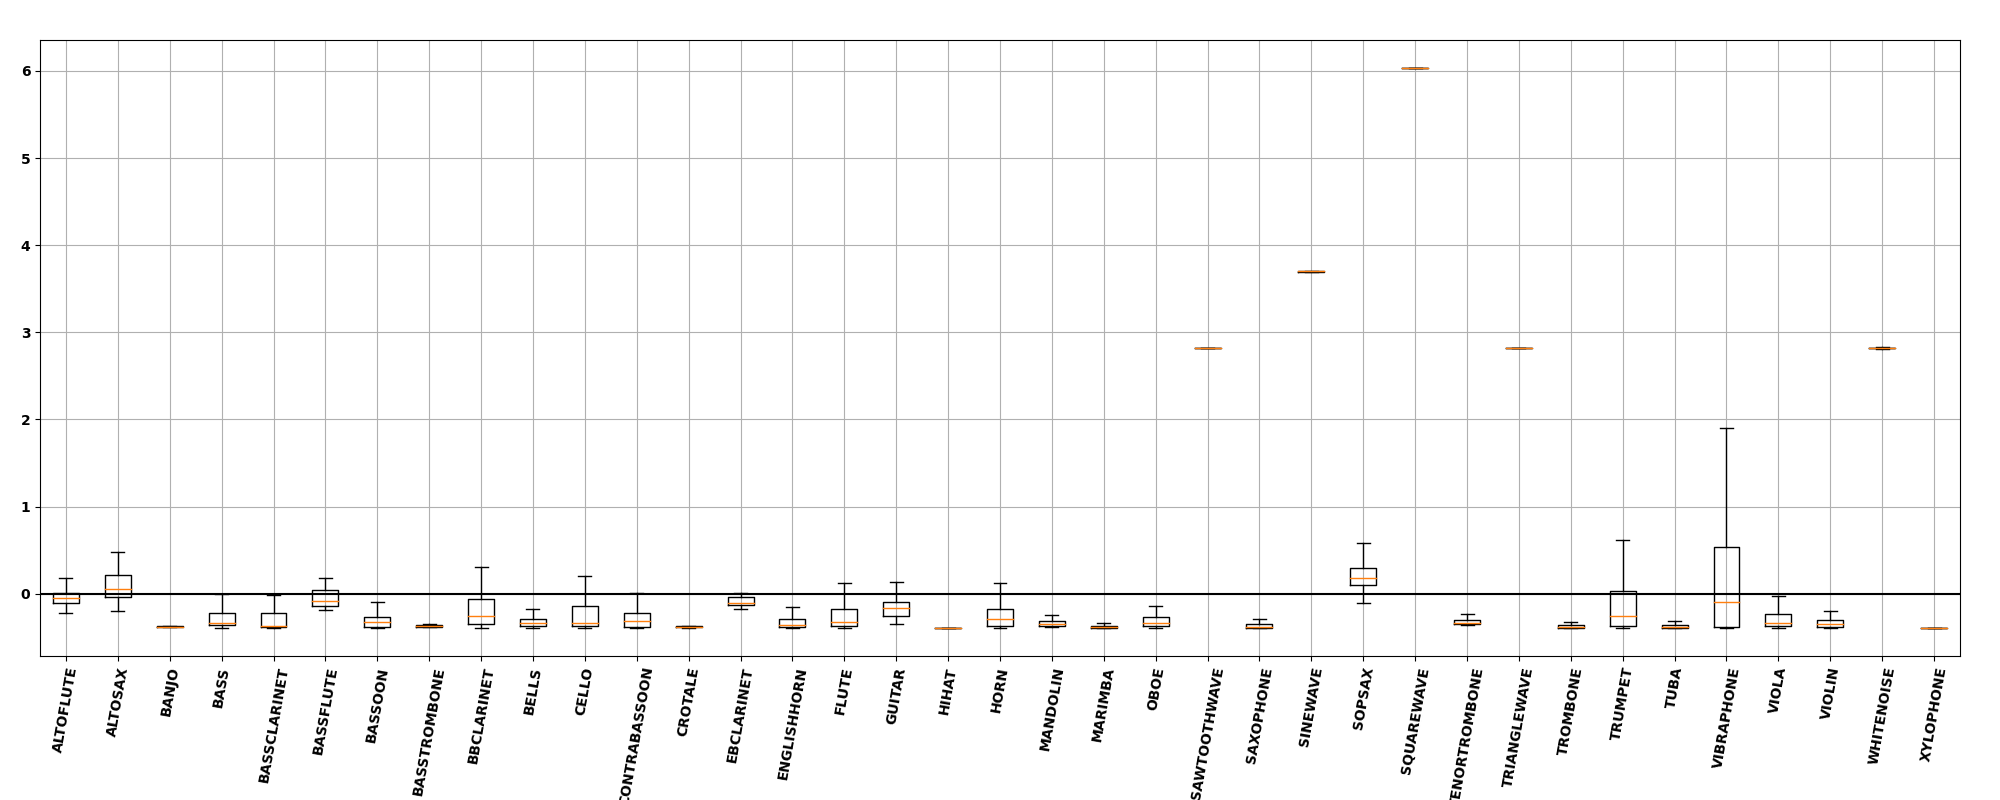
\includegraphics[scale=0.3]{../FiguresFeatures/TCM}
\end{center}
\caption{A comparison of the temporal center mass for each class using a box-and-whisker plot}
\label{fig-FeatureTCM}
\end{figure}

% ================================

\subsubsection{Auto Correlation Coefficients}

\paragraph*{}Auto correlation coefficients (ACC) are rough estimates of the signal spectral distribution. They are computed by multiplying a signal with a time-expedited variant of itself, and then normalized to be between $0$ and $1$ We can compute any number of ACC's and their value changed depending on the index chosen. It is common to use the first $K$ ACC's \cite{Serizel}. For a full waveform signal $s$, with $M$ samples, the $k$-th ACC (indexed from $1$ to $K$) is given by:
\begin{equation}
\label{eqn-FeatureACC}
\text{ACC}_k\big[ s \big] = 
\frac{\sum_{i=0}^{M-k-1}s[i]s[i+k]} {\sqrt{\sum_{i=0}^{M-k-1}s^2[i]} 
\sqrt{\sum_{i=0}^{M-k-1}s^2[i+k]}}
\end{equation}

\paragraph*{}Physically, the numerator of the ACC representing computing the dot product of the signal, $s[i]$ with a time-hastened version of itself $s[i+k]$, and the denominator provides a normalization for the value. Dotting the signal and the time delay allows us to introduce a synthetic phase shift and compare the resulting relationship. If we chose $k$ to be equal, or similar to the number of samples that make-up a period or half-period of the waveform, then $s[i] \approx s[i+k]$ and then $\text{ACC}_k \rightarrow 1$. Alternatively, for many other values of $k$, frequent multiplication and summation of samples that are approximately zero result in $\text{ACC}_k << 1$. This make auto-correlation coefficients extremely useful for detecting periodicity in time-space \cite{Serizel}.

\begin{figure}[H]
\begin{center}


	\begin{subfigure}{1.0\textwidth}
	\centering
	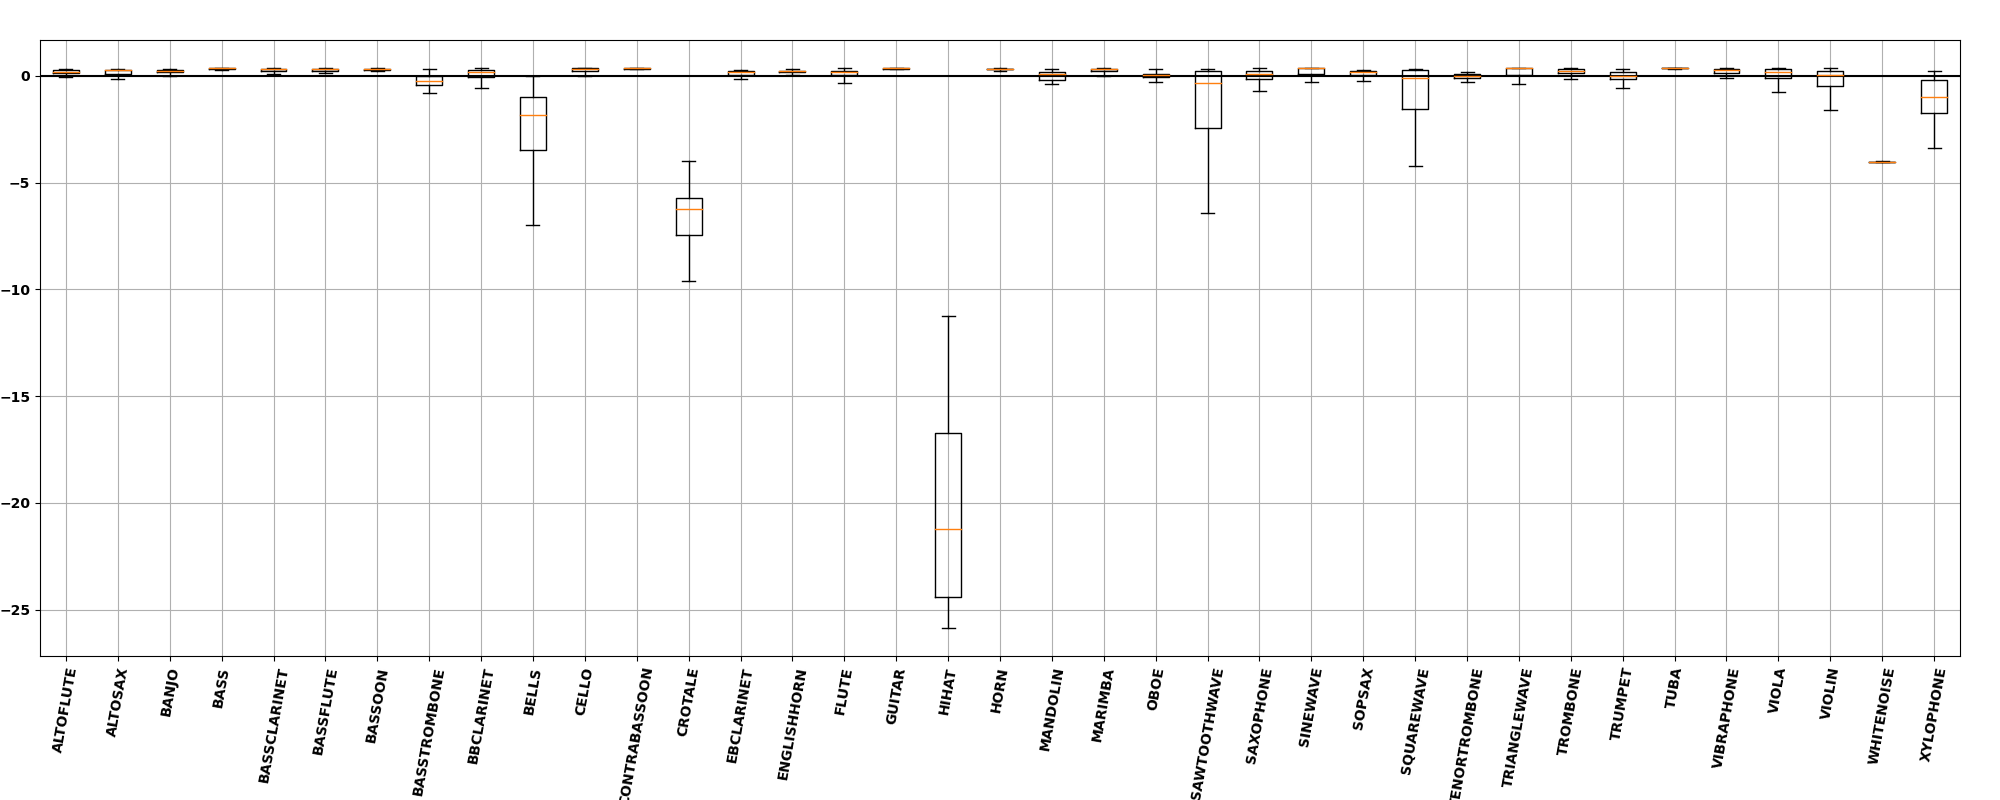
\includegraphics[width=\textwidth , height=0.2\textheight]
		{../FiguresFeatures/ACC_1}
	\caption{ACC $k=1$}
	\end{subfigure}
	
	\begin{subfigure}{1.0\textwidth}
	\centering
	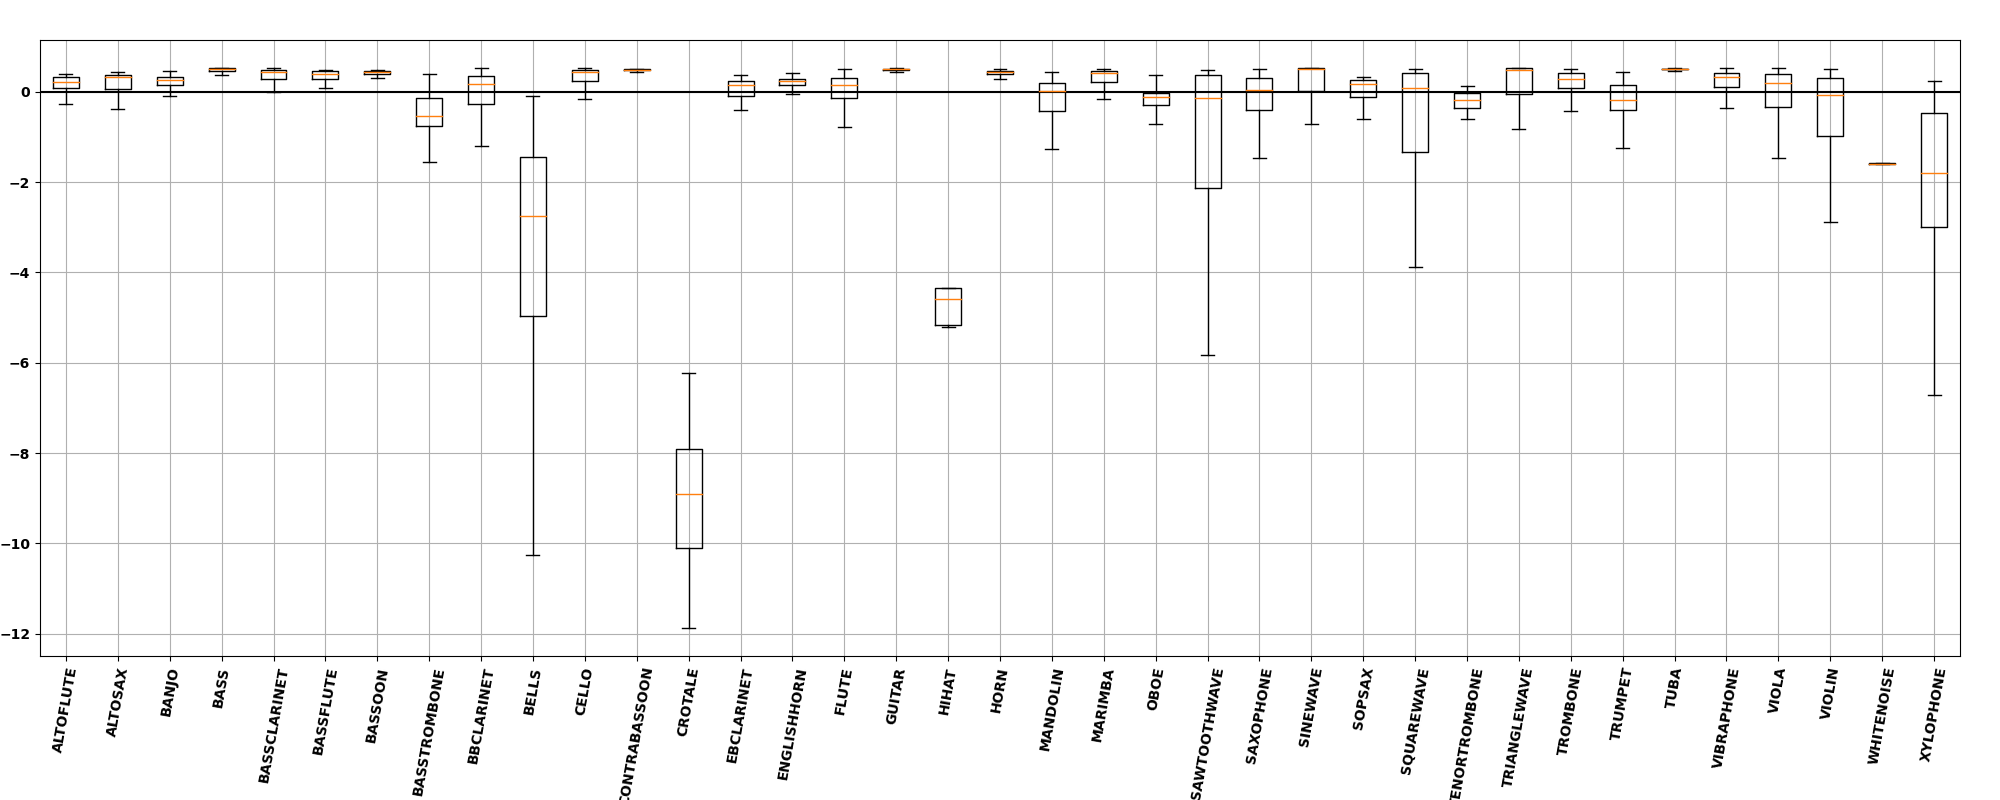
\includegraphics[width=\textwidth , height=0.2\textheight]
		{../FiguresFeatures/ACC_2}
	\caption{ACC $k=2$}
	\end{subfigure}
	
	\begin{subfigure}{1.0\textwidth}
	\centering
	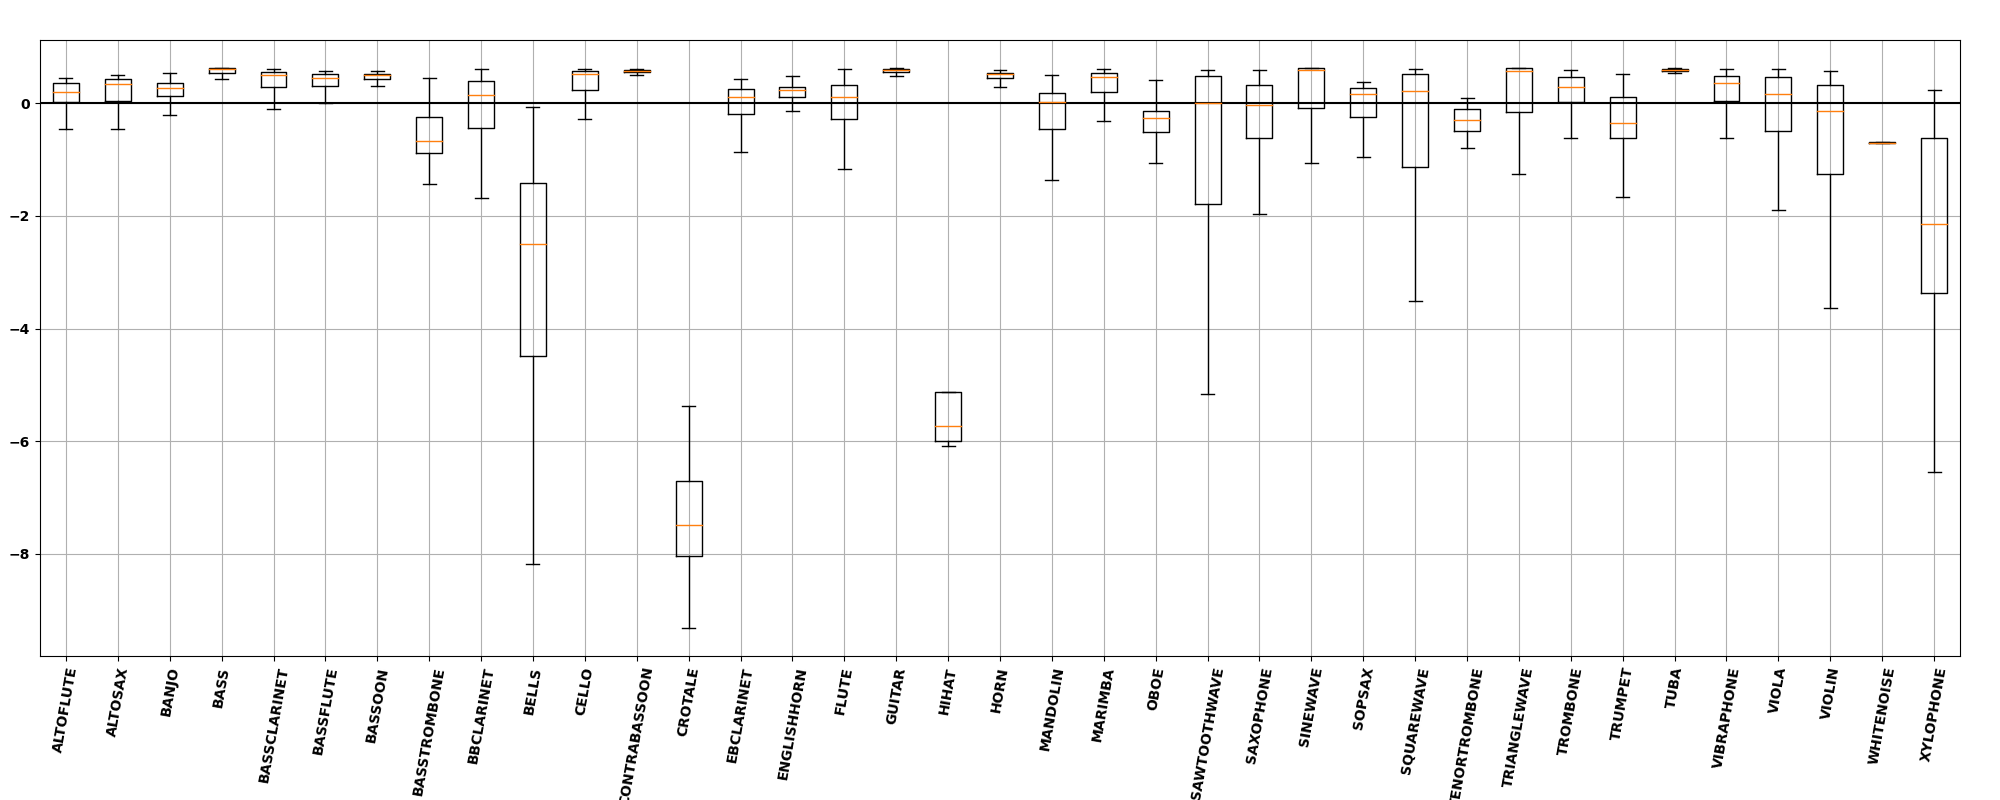
\includegraphics[width=\textwidth , height=0.2\textheight]
		{../FiguresFeatures/ACC_3}
	\caption{ACC $k=3$}
	\end{subfigure}
	
	\begin{subfigure}{1.0\textwidth}
	\centering
	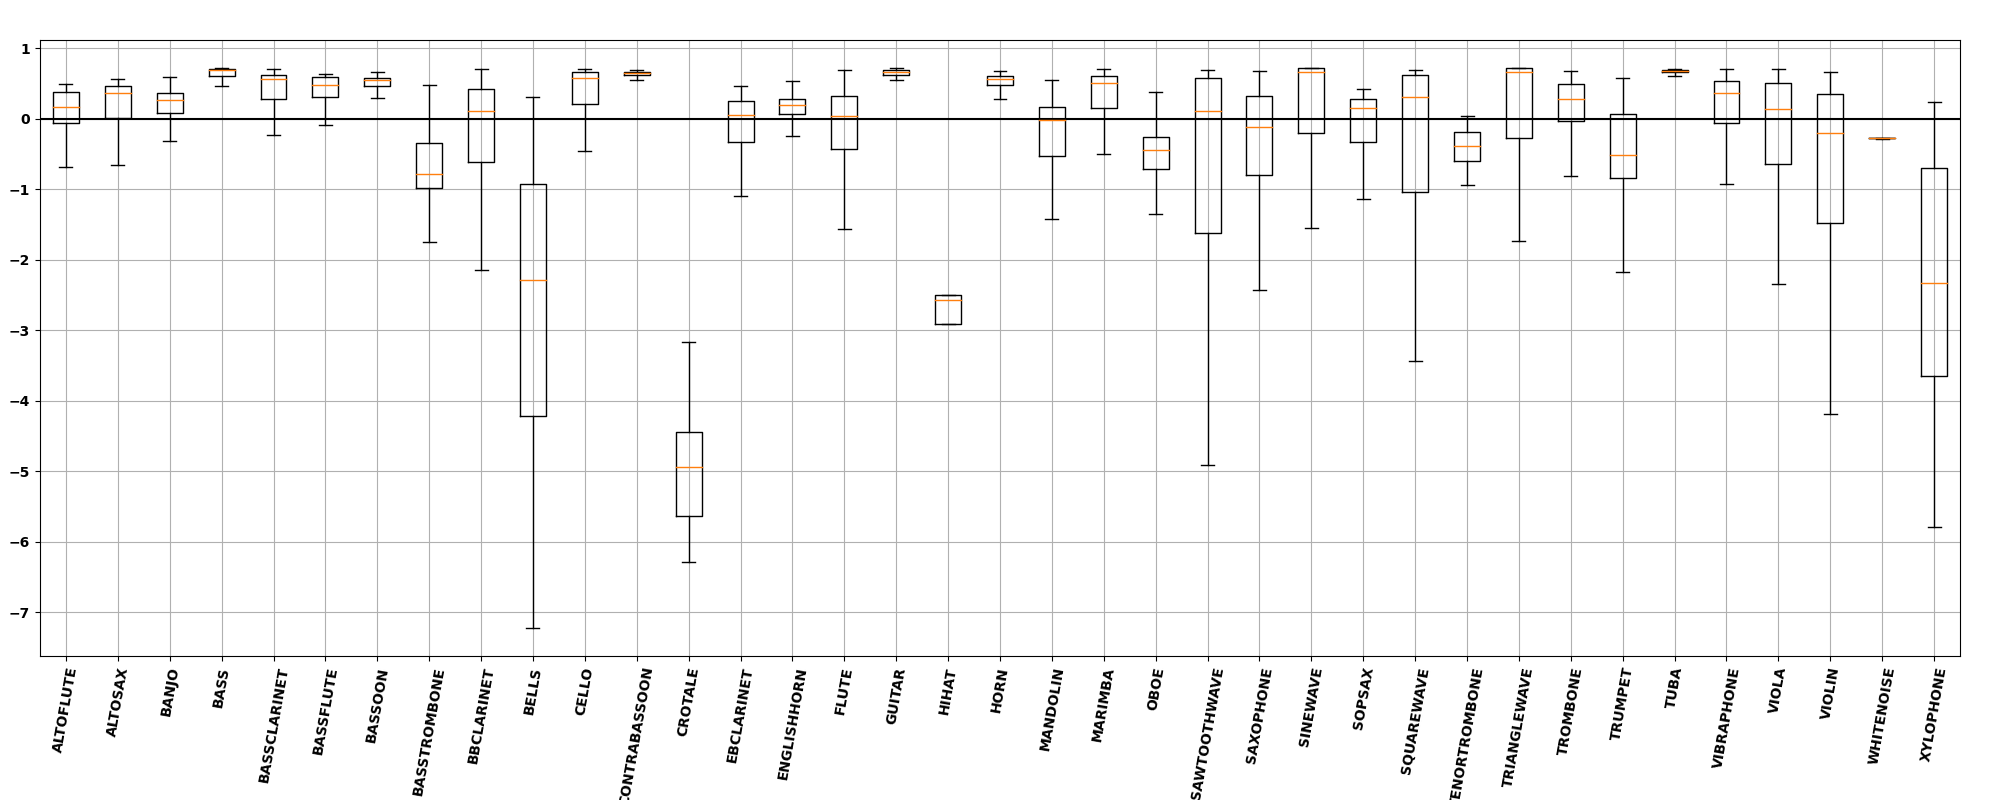
\includegraphics[width=\textwidth , height=0.2\textheight]
		{../FiguresFeatures/ACC_4}
	\caption{ACC $k=4$}
	\end{subfigure}	
	
\end{center}
\caption{A comparison of the first four auto correlation coefficients in each class using box-and-whisker plots}
\label{fig-FeatureACC}
\end{figure}

% ================================================================

\newpage

\subsection{Frequency-Space Features}
\label{subsec-FreqFeatures}

\paragraph*{}The features described in this section are derived from the frequency-domain representations of each audio sample.
For each feature, we detail the physical significance and provide a visualization in feature-space.

\paragraph*{}From frequency space, we use the following $13$ features:
\begin{itemize}
\item[•] Mel Frequency Cepstral Coefficients ($\times 12$)
\item[•] Frequency Center of Mass
\end{itemize}

% ================================

\subsubsection{Mel Filter Bank Energies}

\paragraph*{}Mel Filter Bank Energies (MFBE's) are not used directly as features, but are used in computing Mel Frequency Cepstrum Coefficient (MFCC's) so we describe them here. Mel filter banks are divisions of the frequency spectrum of a signal into $R$ overlapping bins \cite{Sahidullah,Serizel}. These filter banks allows us to group sounds based on their energy distribution in frequency space. Each filter is triangularly shaped, covering a certain band in frequency space, and zero elsewhere. This way, when computing the the dot product of any filter with frequency space, we get an approximation of energy in that filter bank \cite{Sahidullah,Serizel}. 

\paragraph*{}Rather than producing filter banks based on the linear Hertz scale, the frequency axis of the signal is transformed into units of \textit{Mels}, which is used to account for the non-linearity in human pitch perception \cite{Serizel,Khan,Olson}. Filter banks are produced to be evenly spaced on the Mel scale, and then transformed back into the Hertz scale. This has the effect of producing triangular filter banks with grow in width as the frequency increases. The Hertz to Mel and Mel to Hertz transforms are given \cite{Serizel,Khan}:
\begin{equation}
\label{eqn-HztoMel}
M_f[h] = 2595 \log_{10}\big(1+ \frac{h}{700}\big)
\end{equation}
\begin{equation}
\label{eqn-MeltoHz}
H_f[m] = 700 \big(10^{(\frac{m}{2595})}-1\big)
\end{equation}
Where $M_f$ is the frequency in units of Mels, given $[h]$, a frequency in Hertz, and $H_f$ is the frequency in Hertz given $[m]$ a frequency in Mels.


\begin{figure}[H]
\begin{center}
\includegraphics[scale=0.28]{../FiguresSpectrogram/MelFilterBanks}
\end{center}
\caption{Mel Filter Banks shown in frequency space with units of Hertz}
\label{fig-MelFilterBanks}
\end{figure}


\paragraph*{}Each of the $R$ filters is created to be $N'$ samples long, to match the width of the cropped frequency space in the spectrogram, Eq. (\ref{eqn-Spectrogram}). When applied to an analysis frame in the frequency spectrum, the dot-product between the filter and the spectrum gives an approximation of the energy in that filter bank. Each filter is concatenated into a matrix $M$ of shape $R \times N'$, where each row is one filter. We apply the Mel Filter banks to the spectrogram to create matrix $B$:
\begin{equation}
\label{eqn-FilterBanks}
B = (MS)^T
\end{equation}
Matrix $B$ has shape $k \times R$.

\paragraph*{}The matrix product in Eq. (\ref{eqn-FilterBanks}) allows that $B_{i,j}$ is the dot product between the $i$-th analysis frame and the $j$-th filter-bank. Finally, we compute the average energy across all $k$ frames, into array $\widetilde{B}$ with shape $1 \times R$. For this project, we have chosen to use $R = 12$ filter-banks, which are all are used to compute the MFCC's in the next section.

% ================================

\subsubsection{Mel Frequency Cepstral Coeffecients}

\paragraph*{}Ceptstral coefficients are the result of computing the inverse discrete Fourier transform (IDFT) of the logarithm of the frequency Spectrum \cite{Serizel,Sahidullah}. Mel Frequency Cepstral Coefficients (MFCC's) are the most commonly used ceptral coefficients and appear often in digital signal processing. The $c$-th coefficient is given by:
\begin{equation}
\label{feat-MFCC}
\text{MFCC}[c] = \sqrt{\frac{2}{R}} \sum_{i=1}^{R} 
\log\big(\widetilde{B[i]}\big) \cos\bigg(\frac{c(i-\frac{1}{2})\pi}{R[i]}\bigg)
\end{equation}
Where $\widetilde{B}$ is the column average of the Mel filter bank energies computed in Eq. (\ref{eqn-FilterBanks}), and $R$ is the number of filter banks used.

\paragraph*{}Physically, MFCC's are a b inverse transform of a transform. This allows us to investigate the periodicity of the frequency spectrum, which highlights phenomena such as overtones or echoes in the signal \cite{Virtanen}. Cepstrum coefficients are commonly used for speech identification and are very prolific in sound recognition tasks \cite{Serizel,Sahidullah,Liu}. We show a feature-space representation of MFCC's for a selection of coefficients in Fig. (\ref{fig-FeatureMFCCs}).

\begin{figure}[H]
\begin{center}

\begin{subfigure}{1.0\textwidth}
	\centering
	\includegraphics[width=\textwidth , height=0.2\textheight]
		{../FiguresFeatures/MFCC_1}
	\caption{MFCC $R[1]$}
	\end{subfigure}
	
	\begin{subfigure}{1.0\textwidth}
	\centering
	\includegraphics[width=\textwidth , height=0.2\textheight]
		{../FiguresFeatures/MFCC_4}
	\caption{MFCC $R[4]$}
	\end{subfigure}
	
	\begin{subfigure}{1.0\textwidth}
	\centering
	\includegraphics[width=\textwidth , height=0.2\textheight]
		{../FiguresFeatures/MFCC_8}
	\caption{MFCC $R[8]$}
	\end{subfigure}
	
	\begin{subfigure}{1.0\textwidth}
	\centering
	\includegraphics[width=\textwidth , height=0.2\textheight]
		{../FiguresFeatures/MFCC_12}
	\caption{MFCC $R[12]$}
	\end{subfigure}	

\end{center}
\caption{A comparison of 4 Mel Frequency Cepstral Coefficients, $1$, $4$, $8$ and $12$ for each class using box-and-whisker plots}
\label{fig-FeatureMFCCs}
\end{figure}

% ================================

\subsubsection{Frequency Center of Mass}

\paragraph*{}The frequency center-of-mass (FCM) for an audio file provides a representation of how overtones and energy is distributed in the signal's frequency domain. As with the temporal center-of-mass, we treat each column of the $S$ matrix as it's own one-dimensional mass distribution, and compute the center of mass of each column. This encodes the FCM for a single analysis frame (in frequency-space) in the waveform. For an frequency-space analysis frame, $s^{(i)}$, the FCM is given by:
\begin{equation}
\label{eqn-FeatureFCM}
\text{FCM}_{i}\big[ s^{(i)} \big] = \frac{\sum_{j=0}^{N'-1}j s^{(i)}[j]}{\sum_{j=0}^{N'-1}s^{(i)}[j]}
\end{equation}
We compute the FCM for each of the $k'$ frames, and then average the results. We use the average FCM across $k'$ frames to compute the FCM feature:
\begin{equation}
FCM = \frac{1}{k'}\sum_{i=0}^{k'}\text{FCM}_{i}\big[ s^{(i)} \big]
\end{equation}

\paragraph*{}The average FCM gives a strong approximation of the instrument or signal source's range. For example, a flute or violin will have a considerably high FCM value, even in their lower registers. Similarly, basses or tubas will have considerably low FCM values. Given that the standard frequency range of some musical instruments is fixed, it is expected that for any particular instrument, the FCM will consistently have low variability \cite{Olson,White}.

\begin{figure}[H]
\label{fig-FeatureFCM}
\begin{center}
\includegraphics[scale=0.3]{../FiguresFeatures/FCM}
\end{center}
\caption{A comparison of the frequency center of mass for each class using box-and-whisker plots}
\end{figure}

% ================================================================
% ================================================================

\newpage
\section{Evaluating Model Performance}
\label{sec-PerfEval}

\paragraph*{}Before making predictions on unlabeled data such as the Chaotic Synthesizers, we must confirm that our model performs reasonably well on data that it has never interacted with. The most common practice is to divide a full data set into a subset of \textit{training} samples, and \textit{testing} samples \cite{Geron}. As the names imply, the training subset is used to fit the model, and we use the labeled testing data set to evaluate how well the model has trained. The exact ratio of sizes between these subsets varies depending on the task \cite{Goodfellow,Geron2,Mitchell}, however we choose to generally use around $90\%$ training samples and $10\%$ testing samples. If the model performs well within it's training subset, but poorly within the testing subset, this can indicate a model that is \textit{overfitted}, and will not perform well on other unseen samples \cite{Geron}.

% ================================================================

\subsection{K-Folds Cross Validation}
\label{subsec-XValidation}

\paragraph*{}We can expand on the idea of a train/test split with a resampling method called \textit{K-Folds Cross Validation} (Also called X-validation) \cite{Geron,James}. Suppose we have machine learning model $F^*$, with a set of trainable parameters $\Theta$. We also have a data set $X$ and a set of appropriately labeled targets, $Y$, each of which contain $N$ samples. For $K$-folds X-val, we divide the full data set into $K$ subsets (called \textit{folds}), each with size $N/K$:
\begin{equation}
\label{eqn-XValSplit}
X,Y \rightarrow \Big\{ \big(X^{(0)},Y^{(0)}\big) , \big(X^{(1)},Y^{(1)}\big) , ... , \big(X^{(K-1)},Y^{(K-1)}\big) \Big\}
\end{equation}
For each iteration, $k \in [0,1,2,...,K-1]$ we reserve a single subset of data $\big(X^{(k)},Y^{(k)}\big)$ to use as a testing subset. We use the remaining $K-1$ subsets as training data. We fit the model with the data and labels to produce a model $F^{*(k)}$ which as set of parameters $\Theta^{k}$. We return the the test set, and run predictions on this unseen data subset. We compare those predictions to the corresponding set of labels $Y^{(k)}$ and evaluate the result of any selected performance metrics.

\paragraph*{}The output of cross validation is $K$ models that are all trained and evaluated on overlapping subsets of the full data. Each model $F^*$, shows a possible outcome of training the network given a subset of data samples, and a particular set of initial parameters. We can compare the performance of each model and test if they produce similar outcomes, which indicates that the model will be able to consistently generalize to new, unseen samples.

\begin{algorithm}[H]
\caption{A $K$-Fold Cross Validation program.}
\label{alg-CrossValidation}
\begin{algorithmic}
\REQUIRE Untrained Network or related learning algorithm, $F^*$
\REQUIRE A full labeled data set $(X,Y)$ of $N$ samples
\REQUIRE Number of splits in Cross validation, $K$
\REQUIRE Performance metric function(s), $P$

Divide Data into $K$ non-overlapping subsets $x_{i}$, each with roughly $N/K$ samples \\
$X,Y \rightarrow \Big\{ \big(X^{(0)},Y^{(0)}\big) , \big(X^{(1)},Y^{(1)}\big) , ... , \big(X^{(K-1)},Y^{(K-1)}\big) \Big\}$ \\
Performance History $\leftarrow \{\}$

\FOR {$k = 0,1,2,3,...,K-2,K-1$}
	\item Reset all parameters in $F^*$ to a random "untrained" state
	\item Set aside testing data subset
	\item $X_{test} \leftarrow X^{(k)}$
	\item $Y_{test} \leftarrow Y^{(k)}$
	\item Concatenate the remaining subsets into training data set
	\item $X_{train} \leftarrow X^{(i \neq k)}$
	\item $Y_{train} \leftarrow Y^{(i \neq k)}$
	\item Train the model, $F^*$ with the $X_{train}$ and $Y_{train}$ subset.
	\item Evaluate the trained model with the $X_{test}$ and $Y_{test}$ data set, and compute value of metric function(s) $P$
	\item Store Performance $P$ in Performance History array
\ENDFOR \\
Compare performance results, and adjust model or parameters as needed, and repeat if desired. \\
Run additional analysis on performance metrics.
\end{algorithmic}
\end{algorithm}

\paragraph*{}Cross Validation is particularly useful in models such as neural networks because they suffer from the phenomenon of \textit{high-variance}, which means that small changes in initial conditions can drastically change the outcome of the model \cite{James}. Cross validation allows us to control these initial conditions by training the model on similar, but non-identical subsets of data, along with a slightly different set of initial parameters. This repetition allows us to explore the model's behavior over a range of possible initial conditions and validation sets, to ensure that the network is functions as expected over multiple trials. This also eliminates the fear of "unique" cases where the model happens to perform exceptionally well or exceptionally poorly given a random set of initial parameters \cite{Geron}.


% ================================================================

\subsection{Performance Metrics}

\paragraph*{}In the case of the multi-category classifier, it is important that we choose the appropriate performance metrics to confirm that the network is completing it's assigned as as expected \cite{Geron}. While the neural network itself uses the cost function as it's sole objective to optimize, we also require a set of more human-readable functions. For example, an average loss score of $1.075$ over a given subset of previously unseen samples provides us with no real information as to how well the network is performing at it's designed task. In this section, we introduce a set of functions and metrics that allow for a more tangible interpretation of the model's performance. To evaluate any performance metric, we require a set of samples with ground truth labels, $y$, and a model's prediction for those labels, $y^*$ \cite{Goodfellow,James}.

% ================================

\subsubsection{Confusion Matrix}

\paragraph*{}The \textit{standard confusion matrix} (also called a confusion table) is a very quick, often graphical model that can be used to show how a classifier model performs over a subset of predictions. The general idea of this object is count the number of times class $i$ is predicted to be in class $j$, and vice-versa \cite{Geron}. If we see that these classes are being repeatedly \textit{confused} in the model's prediction process, then we can modify the model or features to account for it, or explore why this happens.

\paragraph*{}For a $k$-classes classifier, a confusion matrix will have shape $k \times k$, and every element is a non-negative integer. Each row represents the "ground truth" or  labeled class, and each column represents a predicted class. Thus for a confusion matrix, $C$, we can say that:
\begin{quote}
\label{eqn-ConfMat}
\begin{center}
$C_{i,j} =$ Number of samples that \\ 
belong to class $i$, and were predicted to be in class $j$
\end{center}

\end{quote}
Thus, indexes where $i = j$ represents a correct prediction, and $i \neq k$ indicates an incorrect prediction. A confusion matrix with relatively large values in main diagonal indicates a model that predicts correct labels \cite{Geron}.  Below we present some synthetic confusion matrices, which combine the counts in each index and a corresponding color map.

\begin{figure}[H]

	\begin{subfigure}[b]{0.45\textwidth}
	\centering
	\includegraphics[width=\textwidth]{../FiguresMetrics/StdConfA}
	\caption{Diagonal dominance indicates a stronger classifier}
	\end{subfigure}
	\hfill	\begin{subfigure}[b]{0.45\textwidth}
	\centering
	\includegraphics[width=\textwidth]{../FiguresMetrics/StdConfB}
	\caption{No diagonal dominance indicates a weaker classifier}
	\end{subfigure}
		
\caption{Example Confusion Matrices for $4$-categories classifier}
\label{fig-DummyConfMat}
\end{figure}

\paragraph*{}In addition to the standard confusion matrix, we can also weight entries by prediction score. Rather than adding $+1$ to each entry $C_{i,j}$ where appropriate, we instead add the \textit{probability} value, which is bounded $[0,1]$ (See softmax activation function in section \ref{subsubsec-Softmax})). This allows us to bake in the predictive \textit{confidence} into the confusion matrix. For example, two correct predictions with a score $0.2$ are weighted equally to a single incorrect prediction of $0.4$. This is useful for identifying a classifier that makes correct predictions, but only by smaller threshold. This can almost be through of as assigning "partial credit" to each prediction.

\paragraph*{}However, it is more useful to weight the confusion matrix according to class occurrence. For example, if we had a $2 \times 2$ matrix with entries $100$ and $20$ in the main diagonal, it seems that class $A$ has a much higher prediction success than class $B$. However, if there are $200$ elements in class $A$, and only $21$ in class $B$, then we see that class $A$ has a $50\%$ classification rate, while class $B$ has a $95\%$ classification rate. Consider the list of instrument classes in Fig.(\ref{fig-ClassList}) and notice how all instruments are not equally represented. This creates a training bias such that the model is more heavily trained on a particular class compared to others. This may also show when making predictions, where the classifier is more likely to predict samples that it has been trained on more \cite{James,Loy}. To Combat this, we typically normalize each confusion matrix by the number of samples in each "actual" class. Put simply, we divide each element in a given row by the \textit{sum} of that row.

\paragraph*{}The confusion matrix can be a cumbersome, so often it is useful to express the performance in terms of more concise quantities. For this we use \textit{accuracy score}, \textit{precision score}, \textit{F1-score}, and \textit{recall score}. These metrics are standard in the field of machine-learning classification and are often useful for identifying different strengths and weaknesses in each model \cite{Geron,James}.

% ================================

\subsubsection{Accuracy Score}

\paragraph*{}Accuracy score, while not commonly used is the most intuitive of all of the performance metrics. It is the ratio of correct predictions of he total number of predictions. While immediately useful for equally sampled binary classification problems, it looses meaning as the number of classes increases, and epecially if the number of samples per class is not consistent \cite{Geron}.

\paragraph*{}For example, we could develop a model that uses a few predictors from every human currently alive and determine which of them has walked on the moon. There are roughly 7 billion humans alive, four of which have been on out moon. Simply guess \textit{no} for every human, our model would have more than a $99.9999\%$ accuracy. However, we would argue that this model does not perform well seeing as it has a $0 \%$ recall score, and and a $0 \%$ precision score.

\paragraph*{}Accuracy score of model is defined:
\begin{equation}
\label{eqn-BinaryAccuracy}
\text{Accuracy} = \frac{TP + FN}{TP + FP + FN + FP}
\end{equation}

\paragraph*{}For a multi-class problem, present an accuracy for each individual class, called \textit{micro-accuracy} \cite{James}. The accuracy for a class $j$ is the correct predictions related to the class divided by the total predictions and total counts of the class. We express this mathematically by using sums over each row, each column, and the main diagonal as such:
\begin{equation}
\label{eqn-Accuracy}
\text{Accuracy}_j = \frac{\sum_{i}C_{i,i}}{\sum_{i}C_{i,i} + \sum_{i \neq j}C_{i,j} + \sum_{i \neq j}C_{j,i}}
\end{equation}
Where all sum indexes goes from $0$ to $k-1$.

\paragraph*{}We can also present \textit{global accuracy} or \textit{macro accuracy} by computing the acurracy over the full confusion matrix. This would then by the ratio of all correct predictions (the main diagonal) to all predictions (the sum of the matrix). We can express this as:
\begin{equation}
\text{Accuracy} = \frac{\sum_{i}C_{i,i}}{\sum_{i}\sum_{j}C_{i,j}}
\end{equation}

% ================================

\subsubsection{Precision Score}

\paragraph*{}Precision score (also called \textit{specificity} or \textit{positive predictive value}) is the ratio of chosen elements to all relevant elements. This bounds precision to the range $(0,1)$, with a higher value more desirable. For a classifier with $k = 2$ unique classes, we define the precision score of a model as:
\begin{equation}
\label{eqn-BinaryPrecision}
\text{Prec} = \frac{TP}{TP + FP}
\end{equation}
Where $TP$ is the number of \textit{true-positive}, and $FP$ is the number of false-positive predictions. For a $k$-classes confusion matrix, $C$, the precision score of a class $j$, is given by the entry $C_{j,j}$ divided by the sum of row $j$:
\begin{equation}
\label{eqn-KPrecision}
\text{Prec}_j = \frac{C_{j,j}}{\sum_{i=0}^{k-1}C_{j,i}}
\end{equation}
In the case of a multi-class classifier, the precision score represents a \textit{one-vs-all} measurement. This means that for any class $j$, the sample belongs to class $j$ or it does not. All other classes, $i \neq j$ are temporarily considered to be a single aggregated class. The quantity $TP + FP$, or the sum over the confusion matrix row is a measurement of the total number of items that are predicted to be in the given class. Therefore the precision metric answers the question: \textit{"How many selected items are relevant to the problem?"} \cite{Geron,James}.

% ================================

\subsubsection{Recall Score}

\paragraph*{}Recall score (also called \textit{sensitivity} or \textit{true positive rate}) also offers a more concise performance metric than a confusion metric. For a classifier with $k = 2$ unique classes, we define the recall score of a model as:
\begin{equation}
\label{eqn-BinaryRecall}
\text{Recall} = \frac{TP}{TP + FN}
\end{equation}
Where $TP$ is the number of \textit{true-positive}, and $FN$ is the number of \textit{false-negative} predictions. For a $k$-classes confusion matrix, $C$, the precision score of a class $j$ is given by the entry $C_{j,j}$ divided by the sum of column $j$:
\begin{equation}
\label{eqn-KRecall}
\text{Recall}_j = \frac{C_{j,j}}{\sum_{i=0}^{k-1}C_{i,j}}
\end{equation}
In the case of a multi-class classifier, the recall score also represents a \textit{one-vs-all} measurement. This means that for any class $j$, the sample belongs to class $j$ or it does not. All other classes, $i \neq j$ are again temporarily considered to be a single aggregated class. The quantity $TP + FN$, or the sum over the confusion matrix coumn is a measurement of the total number of items that are actually in the given class. Therefore the recall metric answers the question: \textit{"How many relevant items to the problem are selected?"} \cite{Geron,James}.

% ================================================================

\subsubsection{F1-Score}

\paragraph*{}F1-score (also called F-score) is the harmonic mean of the precision and recall scores and it also bounded on $[0,1]$ with a higher score being favorable \cite{Geron}. Often, the two metrics can be through of as somewhat \textit{exclusive} to each other - the higher one, the lower the other. Compare this with the idea that the more \textit{sensitive} the model is, the less \textit{specific} it is, and vice-versa. This phenomenon is called the \textit{precision-recall tradeoff} \cite{Geron,James}. We compute the $F1$ score for a class $j$ as:
\begin{equation}
\label{eqn-F1Score}
\text{F1}_{j} = 2 \times \frac{\text{Prec}_j + \text{Recall}_j}{\text{Prec}_j \times \text{Recall}_j}
\end{equation}

\paragraph*{}The $F1$ favors models with both a high precision and high recall score. Some models allow for the ability to adjust the threshold of the decision function. This means that by changing a few parameters that are external to the classifier itself, we can change how sensitive or specific a model is when making it's class decision. In the case of this multi-category classifier, this is somewhat like modifying the generated decision boundaries as to change the outputted probability distribution. The $F1$ score to find the set of hyper-parameters that allow for the classifier to produce both a high precision \textit{and} recall score.

% ================================================================

\subsection{Tracking Metrics over a Period of Training}
\label{subsec-TrainingMetrics}

\paragraph*{}A period of training is characterized by fitting the parameters $\Theta$ of a model $F^*$ to a set of data $X$ and corresponding labels $Y$ \cite{Goodfellow,Virtanen}. This is done by passing subsets of data, called \textit{mini-batches}, into the neural network for training. The average cost for the mini-batch is then used to compute the gradient vector $\nabla_{\Theta}J$, and subsequently update the model according to the optimizer chosen \cite{Geron,Goodfellow}. Recall we implement an ADAM optimizer as outlined in section (\ref{subsubsec-Optimizer}).

\paragraph{}We execute training computations in batches to reduce the amount of memory required for the operation. Pushing a full data set through a model at one time would require more RAM than is usually available so we use repeating, non-overlapping subsets of data called mini-batches to avoid memory exhaustion errors. Each mini-batch used equates to one step in the optimizer update rule in Eq. (\ref{eqn-ADAMupdate}) \cite{Goodfellow}. Thus, a single pass over a full data set allows for multiple iterations of the optimizer to reduce the value of the cost function. This can be combined with multiple passes over the full data set, called \textit{epochs} \cite{James,Loy}.

\paragraph*{}Large mini-batches require lots of RAM, but prevent the model from being over-fit to to any one sample, or class of samples. Small mini-batches require less RAM, but often may bias the optimizer to over-fit the given samples, and make optimization unstable \cite{Geron,James}. To ensure that the model is optimizing properly, we can track how the metrics behave over a training period. This allows us to monitor the \textit{rate of convergence} of the model. If the cost function is dropping to quickly or slowly, this may indicate that the optimizer learning rate is too high or too low. This may lead to an over-fit or under-fit model, or indicate an inappropriate set of features are being used \cite{Geron,Goodfellow}. In Some cases, it can be used to initiate \textit{early-stopping}, which halts training when a set of conditions are met. 

\paragraph*{}Given the high dimensionality of this model's parameter space,the large volume of sound files, and the large amount of RAM required to store the spectrogram matrix and the feature vector for each sample, we do not directly load the full data set into memory at once. Instead, we produce a large subset of the full data set of $256$ samples which we dub a \textit{mega-batch}. From this mega-batch, we produce the two design matrices required for input, and load the corresponding labels. We then use a subset of \textit{this} group as the \textit{mini-batches} for training. Each mini-batch contains $32$ samples. Once all mini-batches are fit, we discard the mega-batch design matrices and repeat for the next $256$ samples. 

\paragraph*{}With each training step, we have recorded the precision, recall, and loss scores. These values are computed from the forward pass of the training data before the gradient is computed, and parameters updated, i.e. the program has not seen these particular sample system. Our program stores past metric and loss score histories locally in a \textit{training-history} file, which we can examine after the program completes. Below, we visualize the evolution of each score as training progresses. These plots are from a model that was trained separately on the full data set after cross validation was performed.

\begin{figure}[H]
\begin{center}
\includegraphics[scale=0.3]{../Figures/LossHistory}
\end{center}
\caption{The loss function score decreases with each training step, indicating that optimization is performing correctly}
\label{fig-LossScore}
\end{figure}
similarly, we can visualize the precision score and recall score at each training step.
\begin{figure}[H]
\begin{center}
\includegraphics[scale=0.3]{../Figures/MetricHistory}
\end{center}
\caption{The precision score and recall score generally increase with each training step, indicating that the model is getting both more sensitive and more specific as training progresses}
\label{fig-PrecisionRecallScores}
\end{figure}

\paragraph*{}Notice how loss, precision and recall show a pattern of increasing and decreasing every two steps. This is because we extract a mega-batch of $256$ samples, and perform two epochs of training on the batch. The first step represents the first time the model has seen the data, thus produces a higher cost function value. In the second step, the model has already seen the samples in the batch, and it produces a slightly lower cost value that the first step. The batch is discarded and a new subset of samples is drawn so that the process repeats. With two epochs per mega-batch, and two passes over the full data set (permuted in the middle), the model is effectively trained on the full data set a total of four times.

% ================================================================
% ================================================================

\newpage
\section{Experimental Results}
\label{sec-Results}

\subsection{Executing Cross Validation}

\paragraph*{}To formally produce classification predictions on the chaotic synthesizer waveforms, we must use all of the neural network, physics, and statistical principles outlined in the previous sections. Using the described features in section (\ref{sec-Features}) and appropriate architecture section (\ref{subsec-Architecture}), We run a $K=10$ folds cross validation program as in Alg.(\ref{alg-CrossValidation}). For each of the $10$ models, we produce a standard confusion matrix, and compute the (i) accuracy score, (ii) precision score, (iii) recall score, and (iv) F1 score. In Fig. (\ref{fig-MultimodalXval}) we show how the metrics compare in each the $10$ models by averaging the scores across the $37$ classes.

\begin{figure}[H]
\begin{center}
\includegraphics[scale=0.3]{../FiguresMetrics/AvgXval-Multimodal}
\caption{Performance metrics for the multimodal networks across $10$ models, scores are averaged over $37$ classes}
\label{fig-MultimodalXval}
\end{center}
\end{figure}
Additionally, we present the average standard confusion matrix, and the hits-weighted confusion matrix in Fig. (\ref{fig-MultimodalConfs}).
\begin{figure}[H]
	\begin{subfigure}[b]{0.45\textwidth}
	\centering
	\includegraphics[scale=0.18]{../FiguresMetrics/XValAlphaCLF_Avg_Standard_Confusion}
	\caption{Standard confusion matrix for hybrid network}
	\end{subfigure}
	\hfill
	\begin{subfigure}[b]{0.45\textwidth}
	\centering
	\includegraphics[scale=0.18]{../FiguresMetrics/XValAlphaCLF_Avg_Hits_Weighted_Confusion}
	\caption{Occurrence weighted confusion matrix for hybrid network}
	\end{subfigure}	
	\caption{Confusion matrices, each is averaged over 10 folds of cross validation. Recall that each integer represents a class labeled, as given in Tab. (\ref{fig-ClassList})}
	\label{fig-MultimodalConfs}
\end{figure}

\paragraph*{}We show the metric values of all splits to show the consistency in performance across all subsets. Notice how each split shows reasonable performance as given by the precision and recall score consistently above 80\%. This indicates that for this data set, architecture, and feature selection, our model can accurately classify waveforms and generalize appropriately. This step is critical in ensuring that there are no major out-liers in the classification results, and that any set of initial conditions can still allow the model to reach an acceptable set of parameters and decision boundaries. The results of cross validation indicate a strong classier that can be implemented to make predictions on other waveforms.

% ================================================================

\subsection{Comparing Results between Architectures}

\paragraph*{}In addition to considering our multimodal network architecture performance, we have also run the identical $K = 10$ folds cross validation program on two uni-modal variants of the model. The first variant contains only the Convolutional branch of the network in Fig. (\ref{fig-NetworkArchitecture}), meaning that we feed the activations from the last dense layer in the left column directly to the output layer. Similarly, the second variant contains only the perceptron branch of the network in Fig. (\ref{fig-NetworkArchitecture}), meaning that we feed the activations from the last dense later in the right column directly to the output layer. For consistency, the same full data set (around $18,000$ samples) was using in the cross validation program. Comparing the performance of the each model gives us an insight as to the predictive contribution of each input branch

\begin{figure}[H]
	
	\begin{subfigure}[b]{0.9\textwidth}
	\centering
	\includegraphics[scale=0.3]{../FiguresMetrics/AvgXval-Convolution}
	\caption{Convolutional Unimodal Architecture, see left side of Fig. (\ref{fig-NetworkArchitecture})}
	\end{subfigure}	
	
	\begin{subfigure}[b]{0.9\textwidth}
	\centering
	\includegraphics[scale=0.3]{../FiguresMetrics/AvgXval-Perceptron}
	\caption{Perceptron Unimodal Architecture, see right side of Fig. (\ref{fig-NetworkArchitecture})}
	\end{subfigure}

	\caption{}
	\label{fig-UnimodalXVal}
\end{figure}

\paragraph*{}Compare these unimodal model performances with that of the multimodal network results in Fig. (\ref{fig-MultimodalXval}). Notice how the multimodal network consistently produce superior classification results. Similarly, we present the standard and weighted confusion matrices for both unimodal networks. Compare the results with Fig. (\ref{fig-MultimodalConfs}) and see how the confusion matrix indicates a stronger classifier.

\begin{figure}[H]
	\begin{subfigure}[b]{0.45\textwidth}
	\centering
	\includegraphics[scale=0.18]{../FiguresMetrics/XValGammaCNN_Avg_Standard_Confusion}
	\caption{Standard confusion matrix for the convolution branch}
	\end{subfigure}
	\hfill
	\begin{subfigure}[b]{0.45\textwidth}
	\centering
	\includegraphics[scale=0.18]{../FiguresMetrics/XValGammaCNN_Avg_Hits_Weighted_Confusion}
	\caption{Occurrence weighted confusion matrix for the convolution branch}
	\end{subfigure}	

	\begin{subfigure}[b]{0.45\textwidth}
	\centering
	\includegraphics[scale=0.18]{../FiguresMetrics/XValBetaMLP_Avg_Standard_Confusion}
	\caption{Standard confusion matrix for the perceptron Branch}
	\end{subfigure}
	\hfill
	\begin{subfigure}[b]{0.45\textwidth}
	\centering
	\includegraphics[scale=0.18]{../FiguresMetrics/XValBetaMLP_Avg_Hits_Weighted_Confusion}
	\caption{Occurrence weighted confusion matrix the for perceptron branch}
	\end{subfigure}	
	\caption{Performance metrics for the unimodal networks across $10$ models, scores are averaged over $37$ classes}
	\label{fig-UnimodalConfs}
\end{figure}


% ================================================================

\subsection{Comparing Classification Scores within Each Class}
\label{subsec-ClassScores}

\paragraph*{}Below we present the average accuracy, precision, recall and F1 score for each class, as averaged across $10$-folds cross validation, comparing the three architectures. These plots represent a more "micro" representation of classification by showing the response and scores within each specific class.

% ================================================================

\subsubsection{High Woodwind Scores}

\begin{figure}[H]

	\begin{subfigure}[b]{0.45\textwidth}
	\centering
	\includegraphics[width=\textwidth]{../FiguresClasses/AltoFlute}
	\caption{Alto Flute}
	\end{subfigure}
	\hfill
	\begin{subfigure}[b]{0.45\textwidth}
	\centering
	\includegraphics[width=\textwidth]{../FiguresClasses/AltoSax}
	\caption{Alto Saxophone}
	\end{subfigure}	
	
	\begin{subfigure}[b]{0.45\textwidth}
	\centering
	\includegraphics[width=\textwidth]{../FiguresClasses/BbClarinet}
	\caption{$B\flat$ Clarinet}
	\end{subfigure}	
	\hfill
	\begin{subfigure}[b]{0.45\textwidth}
	\centering
	\includegraphics[width=\textwidth]{../FiguresClasses/EbClarinet}
	\caption{$E\flat$ Clarinet}
	\end{subfigure}	
	
	\begin{subfigure}[b]{0.45\textwidth}
	\centering
	\includegraphics[width=\textwidth]{../FiguresClasses/EnglishHorn}
	\caption{English Horn}
	\end{subfigure}	
	\hfill
	\begin{subfigure}[b]{0.45\textwidth}
	\centering
	\includegraphics[width=\textwidth]{../FiguresClasses/Flute}
	\caption{Flute}
	\end{subfigure}	
	
	\begin{subfigure}[b]{0.45\textwidth}
	\centering
	\includegraphics[width=\textwidth]{../FiguresClasses/Oboe}
	\caption{Oboe}
	\end{subfigure}
	\hfill	
	\begin{subfigure}[b]{0.45 \textwidth}
	\centering
	\includegraphics[width=\textwidth]{../FiguresClasses/SopSax}
	\caption{Soprano Saxophone}
	\end{subfigure}
	
\caption{}
\label{fig-HighWindsScores}
\end{figure}

% ================================================================

\subsubsection{Middle and Low Woodwind Scores}

\begin{figure}[H]
	\begin{subfigure}[b]{0.45\textwidth}
	\centering
	\includegraphics[width=\textwidth]{../FiguresClasses/BassClarinet}
	\caption{Bass Clarinet}
	\end{subfigure}	
	\hfill
	\begin{subfigure}[b]{0.45\textwidth}
	\centering
	\includegraphics[width=\textwidth]{../FiguresClasses/BassFlute}
	\caption{Bass Flute}
	\end{subfigure}	
	
	\begin{subfigure}[b]{0.45\textwidth}
	\centering
	\includegraphics[width=\textwidth]{../FiguresClasses/Bassoon}
	\caption{Bassoon}
	\end{subfigure}	
	\hfill
	\begin{subfigure}[b]{0.45\textwidth}
	\centering
	\includegraphics[width=\textwidth]{../FiguresClasses/ContraBassoon}
	\caption{Contra Bassoon}
	\end{subfigure}	
	
	\begin{subfigure}[b]{0.45\textwidth}
	\centering
	\includegraphics[width=\textwidth]{../FiguresClasses/Saxophone}
	\caption{Tenor Saxophone}
	\end{subfigure}
	
\caption{}
\label{fig-LowWindsScores}
\end{figure}

% ================================================================

\subsubsection{Brass Scores}

\begin{figure}[H]
	\begin{subfigure}[b]{0.45\textwidth}
	\centering
	\includegraphics[width=\textwidth]{../FiguresClasses/BassTrombone}
	\caption{Bass Trombone}
	\end{subfigure}	
	\hfill
	\begin{subfigure}[b]{0.45\textwidth}
	\centering
	\includegraphics[width=\textwidth]{../FiguresClasses/Horn}
	\caption{French Horn}
	\end{subfigure}	
	
	\begin{subfigure}[b]{0.45\textwidth}
	\centering
	\includegraphics[width=\textwidth]{../FiguresClasses/TenorTrombone}
	\caption{Tenor Trombone}
	\end{subfigure}	
	\hfill
	\begin{subfigure}[b]{0.45\textwidth}
	\centering
	\includegraphics[width=\textwidth]{../FiguresClasses/Trombone}
	\caption{Trombone}
	\end{subfigure}	
	
	\begin{subfigure}[b]{0.45\textwidth}
	\centering
	\includegraphics[width=\textwidth]{../FiguresClasses/Trumpet}
	\caption{$B\flat$ Trumpet}
	\end{subfigure}
	\hfill
	\begin{subfigure}[b]{0.45\textwidth}
	\centering
	\includegraphics[width=\textwidth]{../FiguresClasses/Tuba}
	\caption{Tuba}
	\end{subfigure}
	
\caption{}
\label{fig-BrassScores}
\end{figure}

% ================================================================

\subsubsection{String Scores}

\begin{figure}[H]
	\begin{subfigure}[b]{0.45\textwidth}
	\centering
	\includegraphics[width=\textwidth]{../FiguresClasses/Banjo}
	\caption{Banjo}
	\end{subfigure}	
	\hfill
	\begin{subfigure}[b]{0.45\textwidth}
	\centering
	\includegraphics[width=\textwidth]{../FiguresClasses/Bass}
	\caption{Double Bass}
	\end{subfigure}	
	
	\begin{subfigure}[b]{0.45\textwidth}
	\centering
	\includegraphics[width=\textwidth]{../FiguresClasses/Cello}
	\caption{Violoncello}
	\end{subfigure}	
	\hfill
	\begin{subfigure}[b]{0.45\textwidth}
	\centering
	\includegraphics[width=\textwidth]{../FiguresClasses/Guitar}
	\caption{Guitar}
	\end{subfigure}	
	
	\begin{subfigure}[b]{0.45\textwidth}
	\centering
	\includegraphics[width=\textwidth]{../FiguresClasses/Mandolin}
	\caption{Mandolin}
	\end{subfigure}
	\hfill
	\begin{subfigure}[b]{0.45\textwidth}
	\centering
	\includegraphics[width=\textwidth]{../FiguresClasses/Viola}
	\caption{Viola}
	\end{subfigure}
	
	\begin{subfigure}[b]{0.45\textwidth}
	\centering
	\includegraphics[width=\textwidth]{../FiguresClasses/Violin}
	\caption{Violin}
	\end{subfigure}
	
\caption{}
\label{fig-StringScores}
\end{figure}

% ================================================================

\subsubsection{Percussion Scores}

\begin{figure}[H]
	\begin{subfigure}[b]{0.45\textwidth}
	\centering
	\includegraphics[width=\textwidth]{../FiguresClasses/Bells}
	\caption{Bells}
	\end{subfigure}	
	\hfill
	\begin{subfigure}[b]{0.45\textwidth}
	\centering
	\includegraphics[width=\textwidth]{../FiguresClasses/Crotale}
	\caption{Crotales}
	\end{subfigure}	
	
	\begin{subfigure}[b]{0.45\textwidth}
	\centering
	\includegraphics[width=\textwidth]{../FiguresClasses/Hihat}
	\caption{HiHat}
	\end{subfigure}	
	\hfill
	\begin{subfigure}[b]{0.45\textwidth}
	\centering
	\includegraphics[width=\textwidth]{../FiguresClasses/Marimba}
	\caption{Marimba}
	\end{subfigure}	
	
	\begin{subfigure}[b]{0.45\textwidth}
	\centering
	\includegraphics[width=\textwidth]{../FiguresClasses/Vibraphone}
	\caption{Vibraphone}
	\end{subfigure}	
	\hfill
	\begin{subfigure}[b]{0.45\textwidth}
	\centering
	\includegraphics[width=\textwidth]{../FiguresClasses/Xylophone}
	\caption{Xylophone}
	\end{subfigure}	

\caption{}
\label{fig-PercussionScores}
\end{figure}

% ================================================================

\subsubsection{Synthetic Waveform Scores}

\begin{figure}[H]
	\begin{subfigure}[b]{0.45\textwidth}
	\centering
	\includegraphics[width=\textwidth]{../FiguresClasses/SawtoothWave}
	\caption{Sawtooth Wave}
	\end{subfigure}	
	\hfill
	\begin{subfigure}[b]{0.45\textwidth}
	\centering
	\includegraphics[width=\textwidth]{../FiguresClasses/SineWave}
	\caption{Sine Wave}
	\end{subfigure}	
	
	\begin{subfigure}[b]{0.45\textwidth}
	\centering
	\includegraphics[width=\textwidth]{../FiguresClasses/SquareWave}
	\caption{Square Wave}
	\end{subfigure}	
	\hfill
	\begin{subfigure}[b]{0.45\textwidth}
	\centering
	\includegraphics[width=\textwidth]{../FiguresClasses/TriangleWave}
	\caption{Triangle Wave}
	\end{subfigure}	
	
	\begin{subfigure}[b]{0.45\textwidth}
	\centering
	\includegraphics[width=\textwidth]{../FiguresClasses/WhiteNoise}
	\caption{White Noise}
	\end{subfigure}	


\caption{}
\label{fig-SynthScores}
\end{figure}

% ================================================================

\subsection{Discussion of Results}

\paragraph*{}Comparing the results within each class, as averaged over $10$ folds of cross validation indicates that our model performs very well at the ability to a match a sound waves in digital audio files to their sources. We see this behavior in the plots in section (\ref{subsec-ClassScores}) as well as the confusion matrices in Fig. (\ref{fig-MultimodalConfs}). For the chosen set of classes, features and architecture, the model can generalize to new information allowing it to distinguish between different types of musical instruments reasonably well for samples that it has not yet interacted with. Additionally, we show that the predictive power of the model improves through our development of the multimodal architecture. By choosing to express the audio file contents in two different modalities of the spectrogram matrix and the feature vector, the hybrid model demonstrates a generally higher classification performance across the same number of samples and splits. 

\paragraph*{}Despite the higher average scores in the hybrid network, see Fig. (\ref{fig-MultimodalXval}) compared to each unimodal network, Fig. (\ref{fig-UnimodalXVal}), some exceptions do arise at a micro-level (within each class). Consider the Hi-hat instrument in Fig. (\ref{fig-PercussionScores}c). Over the cross validations, it was found that the multilayer perceptron architecture produced a better precision, recall, and F1 score than either the convolution or the hybrid network architecture. This can be contrasted with most other classes showing that the hybrid model performed better than either individual mode, with the convolution architecture as a close second. 

\paragraph*{}While the hybrid model can differentiate between many types of instruments, each unimodal variant shows slightly less success over the full data set. In many instances, the MLP-only architecture particularly shows unstable and inconsistent performance. For certain instruments like the $E\flat$ clarinet, tenor saxophone, tenor trombone, and hi-hat, the feature vector does a very poor job of isolating and identifying those classes. However, for instruments such as the soprano saxophone, tuba, and square wave, the feature-vector allows the MLP to perform very reasonably. We see a similar imbalance with the CNN-only architecture where classes such as alto flute, bass flute, bass trombone, and mandolin show poor classification rates. This can be contrasted with English horn, tuba, bells, and double bass, where a much higher classification performance is found. Further exploration is required to provide a full explanation and justification of why this wide range of performance is observed.

\paragraph*{}We can also observe a loose correlation to the number of samples in each class compared to the classification metric scores. When a model is trained on one class more than another we are more likely to generate predictions for that class too. This can be seen in the scores and occurrences of alto flutes (\ref{fig-HighWindsScores}a) with $72$ samples compared to that of English horns (\ref{fig-HighWindsScores}e) with $1382$ samples. In both confusion matrices of Fig. (\ref{fig-MultimodalConfs}), we see a relatively small entry in $C_{0,0}$ (alto flutes) compared to $C_{14,14}$ ( English horn). This indicates that fewer correction predictions were made, and the normalized matrix shows that fewer predictions were made at all. Contrast this with the English horn having a dark red square in both matrices shows many predictions, and many correction predictions. Future work could explore how classification performance would be affected when weighting each class inversely to it's number of samples in the data set. This would allow each class to be weighted uniformly in the training process and may potentially mitigate some of the variability of the performances across classes.

\paragraph*{}Future work on this project would benefit from a further exploration and development of input features. While the ability to discern classes is present, classification scores are still unstable and we observe a wide range of performances. To combat this, we would produce additional feature that convey characteristic properties of the digital audio files that allow for the generation of more distinctive decision boundaries. In addition to new features, it would be beneficial to further study the distribution of samples in feature space and execute some form of $K$-best features algorithm. This would indicate which of the  chosen predictors consistent or inconsistent with our requirements of intra-class and inter-class variability. 

\paragraph*{}In addition to input features, it may be beneficial to group for the the related classes together. For example, violins and violas have very similar physical constructions, have very similar formant structures, and thus have very similar behaviors in our feature-space. As a result, some humans may also have difficulty differentiating the two, so it may be forgiven that a classification neural network would do the same. We can also consider grouping range variants of parent instruments such as flutes, alto flutes, bass flutes into a single \textit{flutes} category. It is possible that the new distribution of properties in feature-space may also warrant the development of a new set of predictors again. 

\paragraph*{}Finally as a practical demonstration, future work entails the deployment of this classifier to generally unlabeled audio samples, provided that they have the same format. In particular, we would like to explore how classification would behave when testing it on digitally generated chaotic synthesizer wave forms. These signals are representations of chaotic systems that resemble some of the acoustic the periodic properties of digital audio waveforms. By using the automated classifier, we would like to test the versatility of the classifier when subject to samples that may differ drastically in oame ways from the training data set. This demonstration would be a fantastic exploration into the ability for the model to generalize, and the strength of the learned function parameters.

% ================================================================
% ================================================================

\newpage
\section{Conclusion}
\label{sec-Conclusion}

\paragraph*{}The experimental results show that we have successfully constructed a multimodal neural network that can classify sound waves into one of $37$ categories that it most resembles. Each category is representative of a particular musical instrument, and collectively the categories cover many stringed, woodwind, brass, mallet percussion, and synthetic instruments. From performing a $10$-folds cross validation, we find that given slightly different initial conditions and overlapping subsets of training data, the model produces consistency reasonable classification scores as shown in Fig. (\ref{fig-MultimodalXval}). This behavior indicates a neural network architecture and features that can generalize to unseen data samples.

\paragraph*{}Examining the two diagonally dominant confusion matrices in Fig. (\ref{fig-MultimodalConfs}) indicates that the neural network is consistently making correct categorical predictions. The presence of off-diagonal entries in the confusion matrices indicates that misclassifications are a common possibility. Averaged across $37$ classes, we see in Fig. (\ref{fig-MultimodalXval}) that the classification accuracy score averages around $0.98$ and precision and recall scores around $0.83$ and $0.82$ respectively. This means that examining each class in an \textit{one-versus-all} context, the model selects more than $83\%$ of relevant samples, and more than $82\%$ of relevant samples are selected. This indicates that the multimodal neural network that can reasonably differentiate between $37$ classes of musical instruments.

\paragraph*{}We conclude that on average, the hybrid neural network architecture in Fig. (\ref{fig-NetworkArchitecture}) exhibits superior classification performance over either of it's unimodal counterpart architectures. In examining confusion matrices from both unimodal models in Fig. (\ref{fig-UnimodalConfs}), we see the presence of diagonal dominance. However, in comparing this to the multimodal network confusion matrix from Fig. (\ref{fig-MultimodalConfs}), we see that the multimodal network has a much more pronounced main diagonal. This indicates that by aggregating to the output of each modal branch with a concatenation layer, we can benefit from the predictive power of both architectures together.

% ================================================================
% ================================================================

\newpage
\section{Acknowledgments}
\label{sec-Acknowledge}

\paragraph*{}The completion of this project would not have been possible without the various contributions from the following people and organizations:

\begin{itemize}

\item[•]Dr. Kevin Short and Dr. Maurik Holtrop for advising this project.

\item[•]Dakota Buell, Tan Dao, Nathan Richard, and Morgan Saidel for consultation on physics, mathematics, and programming topics.

\item[•]Madeline Edwards and John Parker for differing me to this project, as well as constant support and consultation on mathematical topics.

\item[•]Dr. Kourosh Zarringhalam and Dr. Marek Petrik for additional consultation on machine learning topics.

\item[•]University of Iowa, Electronic Music Studio and Philharmonia Symphony Orchestra for the digital sound library used for training data samples.

\end{itemize}

% ================================================================
% ================================================================

\newpage

\begin{thebibliography}{9}
\bibliographystyle{apalike}

\bibitem{Bishop}
Bishop, Christopher M. \textit{Pattern Recognition and Machine Learning}. Springer New York, 2016. 

\bibitem{Geron}
Geron, Aurelien. \textit{Hands-on Machine Learning with Scikit-Learn and TensorFlow: Concepts, Tools, and Techniques to Build Intelligent Systems}. O'Reilly, 2017.

\bibitem{Geron2}
Geron, Aurelien. \textit{Hands-on Machine Learning with Scikit-Learn and TensorFlow: Concepts, Tools, and Techniques to Build Intelligent Systems}. 2nd ed., O'Reilly, 2019.

\bibitem{Goodfellow}
Goodfellow, Ian, et al.\textit{Deep Learning}. MIT Press, 2017.

\bibitem{Haberman}
“Wave Equation: Vibrating Strings and Membranes.” \textit{Applied Partial Differential Equations with Fourier Series and Boundary Value Problems}, by Richard Haberman, Pearson, 2019, pp. 130–150. 

\bibitem{Hornbostel}
Von Hornbostel, Erich, and Curt Sachs. “Classification of Musical Instruments.” \textit{The Galpin Society Journal}, Translated by Anthony Baines and Klaus Wachsmann, vol. 14, Mar. 1961, pp. 3–29. 

\bibitem{Hunter}
Hunter, Joseph L. \textit{Acoutics}. Prentice Hall, 1957. 

\bibitem{James}
James, Gareth, et al. \textit{An Introduction to Statistical Learning with Applications in R}. Springer, 2017.

\bibitem{Khan}
Khan, M. Kashif Saeed, and Wasfi G. Al-Khatib. “Machine-Learning Based Classification of Speech and Music.” Multimedia Systems, vol. 12, no. 1, 2006, pp. 55–67., doi:10.1007/s00530-006-0034-0.

\bibitem{Levine}
Levine, Daniel S. \textit{Introduction to Neural and Cognitive Modeling}. 2nd ed., Routledge, 2000.

\bibitem{Li}
Li, Yingming, and Ming Yang. “A Survey of Multi-View Representation Learning.” Journal of LateX Class Files, vol. 14, no. 8, Aug. 2015. 

\bibitem{Liu}
Liu, Zhu, et al. "Audio Feature Extraction and Analysis for Scene Segmentation and Classification." Journal of VLSI Signal Processing, vol. 20, 1998, pp. 61–79.

\bibitem{Loy}
Loy, James , \textit{Neural Network Projects with Python}. Packt Publishing, 2019

\bibitem{Matplotlib}
John D. Hunter. Matplotlib: A 2D Graphics Environment, Computing in Science \& Engineering, 9, 90-95 (2007), DOI:10.1109/MCSE.2007.55

\bibitem{McCulloch}
McCulloch, Warren S., and Walter Pitts. "A Logical Calculus of the Ideas Immanent in Nervous Activity." \textit{The Bulletin of Mathematical Biophysics}, vol. 5, no. 4, 1943, pp. 115–133.

\bibitem{Mierswa}
Mierswa, Ingo, and Katharina Morik. "Automatic Feature Extraction for Classifying Audio Data." \textit{Machine Learning}, vol. 58, no. 2-3, 2005, pp. 127–149., doi:10.1007/s10994-005-5824-7.

\bibitem{Mitchell}
Mitchell, Tom Michael. Machine Learning. 1st ed., McGraw-Hill, 1997.

\bibitem{Ngiam}
Ngiam, Jiquan, et al. "Multimodal Deep Learning." 2011. 

\bibitem{Numpy}
Harris, C.R., Millman, K.J., van der Walt, S.J. et al. Array programming with NumPy. Nature 585, 357–362 (2020). DOI: 0.1038/s41586-020-2649-2. 

\bibitem{Olson}
Olson, Harry E. \textit{Music, Physics and Engineering}. 2nd ed., Dover Publications, 1967.

\bibitem{Peatross}
Peatross, Justin, and Michael Ware. \textit{Physics of Light and Optics.} Brigham Young University, Department of Physics, 2015.

\bibitem{Petrik}
Petrik, Marek. "Introduction to Deep Learning." Machine Learning. 20 April. 2020, Durham, New Hampshire.

\bibitem{Philharmonia}
Philharmonia Symphony Orchestra home page- \textit{https://philharmonia.co.uk/}

\bibitem{Powers}
Powers, David. (2008). \textit{Evaluation: From Precision, Recall and F-Factor to ROC, Informedness, Markedness \& Correlation}. Mach. Learn. Technol. 2. 

\bibitem{Sahidullah}
Sahidullah, Goutam S. “Design, Analysis and Experimental Evaluation of Block Based Transformation in MFCC Computation for Speaker Recognition.” 18 Nov. 2011. 

\bibitem{Serizel}
Serizel, Roman, et al. “Acoustic Features for Environmental Sound Analysis.” Computational Analysis of Sound Scenes and Events, by Tuomas Virtanen, Springer, 2018, pp. 71–101. 

\bibitem{Scipy}
Pauli Virtanen, et. al. SciPy 1.0: Fundamental Algorithms for Scientific Computing in Python. Nature Methods, 17(3), 261-272.

\bibitem{Short}
Short, K. and Garcia R.A. 2006. "Signal Analysis Using the Complex Spectral Phase Evolution (CSPE) Method." AES: \textit{Audio Engineering Society Convention Paper}.

\bibitem{Sklearn}
Fabian Pedregosa, et. al. Scikit-learn: Machine Learning in Python, Journal of Machine Learning Research, 12, 2825-2830 (2011) 

\bibitem{Taylor}
“Continuum Mechanics.” \textit{Classical Mechanics}, by John Robert Taylor, University Science Books, 2005, pp. 681–738. 

\bibitem{Tensorflow}
TensorFlow: Large-scale machine learning on heterogeneous systems,
2015. Software available from tensorflow.org.

\bibitem{Virtanen}
Virtanen, Tuomas, et al. \textit{Computational Analysis of Sound Scenes and Events.} Springer, 2018.

\bibitem{UnivIowa}
University of Iowa Electronic Music Studios home page- \textit{http://theremin.music.uiowa.edu/}

\bibitem{White}
White, Harvey Elliott, and Donald H. White. \textit{Physics and Music: the Science of Musical Sound}. Dover Publications, Inc., 2019.

\bibitem{Zhang}
Zhang, Tong, and C.-C. Jay Kuo. “Content-Based Classification and Retrieval of Audio.” \textit{Advanced Signal Processing Algorithms, Architectures, and Implementations VIII}, 2 Oct. 1998, pp. 432–443., doi:10.1117/12.325703.

\end{thebibliography}

% ================================================================

\end{document}